% !TeX program = xelatex
% !TeX encoding = UTF-8
% ============================================================
% 热能动力工程·期中总结（SJTUBeamer 扩充版）
% 编译：latexmk -xelatex -interaction=nonstopmode -halt-on-error main.tex
% ============================================================
\documentclass[aspectratio=169,fontset=fandol,10pt]{ctexbeamer}

\usepackage{amsmath,amssymb,bm}
\usepackage{booktabs,tabularx,array,multirow,makecell}
\usepackage{graphicx,calc,etoolbox}
\usepackage{multicol}
\usepackage{ragged2e}
\usepackage{pgfplots}
\usepgfplotslibrary{fillbetween}
\pgfplotsset{compat=1.18}

\usetheme[min,red,light,infolines,topright]{sjtubeamer}
% ============================================================
% 版式、颜色与自定义命令
% 本文件只作用于项目副本，不修改原 SJTUBeamer 模板
% ============================================================

% ---------- 字体与字号 ----------
\usefonttheme{professionalfonts}
\setbeamerfont{frametitle}{size=\fontsize{12.3}{15.0}\selectfont,series=\bfseries}
\setbeamerfont{framesubtitle}{size=\fontsize{8.5}{10}\selectfont}
\setbeamerfont{normal text}{size=\fontsize{9.6}{12.8}\selectfont}
\setbeamerfont{itemize/enumerate body}{size=\fontsize{9.6}{12.8}\selectfont}
\setbeamerfont{itemize/enumerate subbody}{size=\fontsize{8.8}{11.4}\selectfont}
\setbeamerfont{footline}{size=\fontsize{6.8}{8.0}\selectfont}
\setbeamerfont{caption}{size=\fontsize{7.2}{9.0}\selectfont}
\setbeamerfont{block title}{size=\fontsize{9.2}{11.2}\selectfont,series=\bfseries}
\setbeamerfont{block body}{size=\fontsize{9.0}{11.8}\selectfont}

% ---------- 页面边距与段落 ----------
\setbeamersize{text margin left=7mm,text margin right=7mm}
\setlength{\parindent}{0pt}
\setlength{\parskip}{1.1pt}
\setlength{\leftmargini}{1.25em}
\setlength{\leftmarginii}{1.0em}
\setlength{\itemsep}{2.2pt}
\setlength{\tabcolsep}{3.2pt}
\renewcommand{\arraystretch}{1.13}
\setlength{\abovedisplayskip}{4pt}
\setlength{\belowdisplayskip}{4pt}
\setlength{\abovedisplayshortskip}{2pt}
\setlength{\belowdisplayshortskip}{2pt}

% ---------- 主题附加颜色 ----------
\definecolor{cblue}{HTML}{245B73}
\definecolor{cbluepale}{HTML}{EEF5F8}
\definecolor{camber}{HTML}{A96600}
\definecolor{camberpale}{HTML}{FFF6E6}
\definecolor{cgreen}{HTML}{35664C}
\definecolor{cgreenpale}{HTML}{F0F7F2}
\definecolor{cgray}{HTML}{4F5B66}
\definecolor{cgraypale}{HTML}{F4F6F7}

% 页码与页脚
\setbeamertemplate{page number in head/foot}{\insertframenumber/\inserttotalframenumber}
\setbeamerfont{page number in head/foot}{size=\fontsize{7.0}{8.2}\selectfont}

% ---------- 标题中的原页标记 ----------
\newcommand{\src}[2]{%
  \texorpdfstring{\textcolor{cprimary}{原第 #1 页}\enspace\textcolor{black!35}{$\mid$}\enspace #2}%
  {原第 #1 页｜#2}}
\newcommand{\srcsupp}[2]{%
  \texorpdfstring{\textcolor{cprimary}{原第 #1 页补充}\enspace\textcolor{black!35}{$\mid$}\enspace #2}%
  {原第 #1 页补充｜#2}}

% ---------- 小标签 ----------
\newcommand{\tagtext}[2]{%
  \tikz[baseline=(t.base)]{\node[fill=#1,text=white,rounded corners=1pt,
    inner xsep=3.2pt,inner ysep=1.1pt,font=\fontsize{6.8}{7.6}\selectfont\bfseries] (t) {#2};}}
\newcommand{\srctag}{\tagtext{cprimary}{原课件}}
\newcommand{\addtag}{\tagtext{cblue}{补充}}
\newcommand{\readtag}{\tagtext{camber}{阅读提示}}

% ---------- 信息盒 ----------
\tcbuselibrary{breakable,skins}
\newtcolorbox{keybox}[1]{%
  enhanced,breakable=false,
  colback=cprimary!4!white,colframe=cprimary!70!black,
  boxrule=0pt,leftrule=1.7pt,arc=1.2pt,
  left=5.5pt,right=5.5pt,top=3.2pt,bottom=3.2pt,
  fonttitle=\small\bfseries,coltitle=cprimary!75!black,
  title={#1},titlerule=0pt,
  before skip=3pt,after skip=3pt
}
\newtcolorbox{bluebox}[1]{%
  enhanced,breakable=false,
  colback=cbluepale,colframe=cblue,
  boxrule=0pt,leftrule=1.7pt,arc=1.2pt,
  left=5.5pt,right=5.5pt,top=3.2pt,bottom=3.2pt,
  fonttitle=\small\bfseries,coltitle=cblue,
  title={#1},titlerule=0pt,
  before skip=3pt,after skip=3pt
}
\newtcolorbox{amberbox}[1]{%
  enhanced,breakable=false,
  colback=camberpale,colframe=camber,
  boxrule=0pt,leftrule=1.7pt,arc=1.2pt,
  left=5.5pt,right=5.5pt,top=3.2pt,bottom=3.2pt,
  fonttitle=\small\bfseries,coltitle=camber,
  title={#1},titlerule=0pt,
  before skip=3pt,after skip=3pt
}
\newtcolorbox{plainbox}{%
  enhanced,breakable=false,
  colback=white,colframe=black!18,
  boxrule=0.4pt,arc=1.2pt,
  left=5pt,right=5pt,top=3pt,bottom=3pt,
  before skip=3pt,after skip=3pt
}

% 小号表格环境
\newcolumntype{Y}{>{\raggedright\arraybackslash}X}
\newcolumntype{C}{>{\centering\arraybackslash}X}
\newenvironment{smalltab}{\par\vspace{1pt}\centering\fontsize{8.2}{10.2}\selectfont}{\par\vspace{1pt}}
\newenvironment{tinytab}{\par\vspace{1pt}\centering\fontsize{7.3}{9.0}\selectfont}{\par\vspace{1pt}}

% ---------- TikZ 通用样式 ----------
\usetikzlibrary{arrows.meta,positioning,calc,fit,backgrounds,shapes.geometric,
  decorations.pathreplacing,decorations.markings,patterns}
\tikzset{
  >={Stealth[length=2.1mm,width=1.4mm]},
  arr/.style={-{Stealth[length=2.1mm,width=1.4mm]},draw=cprimary!85,thick},
  arrb/.style={-{Stealth[length=2.1mm,width=1.4mm]},draw=cblue,thick},
  flow/.style={-{Stealth[length=2.0mm,width=1.3mm]},draw=cgray,thick},
  thinarr/.style={-{Stealth[length=1.6mm,width=1.1mm]},draw=black!55,thin},
  box/.style={draw=cprimary!60,fill=cprimary!5,rounded corners=1.4pt,
    align=center,inner sep=3.2pt,font=\fontsize{7.6}{9.1}\selectfont,
    minimum height=7.6mm},
  boxb/.style={draw=cblue!65,fill=cbluepale,rounded corners=1.4pt,
    align=center,inner sep=3.2pt,font=\fontsize{7.6}{9.1}\selectfont,
    minimum height=7.6mm},
  boxg/.style={draw=black!25,fill=cgraypale,rounded corners=1.4pt,
    align=center,inner sep=3.2pt,font=\fontsize{7.4}{8.9}\selectfont,
    minimum height=7.4mm},
  lab/.style={font=\fontsize{6.8}{8.2}\selectfont,inner sep=1.2pt,align=center},
  labb/.style={font=\fontsize{6.8}{8.2}\selectfont,inner sep=1.2pt,align=center,text=cblue!80!black},
  dim/.style={draw=black!55,thin},
  axis/.style={-{Stealth[length=1.8mm]},draw=black!70,thin},
  dashline/.style={draw=black!40,dashed,thin},
  hline/.style={draw=cprimary!45,thin}
}

% ---------- 结构/示意图常用小命令 ----------
\newcommand{\hot}[1]{\textcolor{cprimary!85!black}{\textbf{#1}}}
\newcommand{\cold}[1]{\textcolor{cblue}{\textbf{#1}}}
\newcommand{\unit}[1]{\,\mathrm{#1}}
\newcommand{\dd}{\mathrm{d}}
\newcommand{\ex}{\mathrm{ex}}
\newcommand{\fw}{\mathrm{fw}}
\newcommand{\ms}{\mathrm{ms}}
\newcommand{\rh}{\mathrm{rh}}
\newcommand{\net}{\mathrm{net}}
\newcommand{\opt}{\mathrm{opt}}

% 章节封面：编号、标题、英文副题、三条主线
\newcommand{\chapterintro}[5]{%
  \begin{columns}[T,onlytextwidth]
    \begin{column}{0.285\textwidth}
      \begin{tcolorbox}[enhanced,colback=cprimary!7,colframe=cprimary!7,
        arc=2pt,left=3pt,right=3pt,top=7pt,bottom=7pt,halign=center]
        {\fontsize{40}{43}\selectfont\bfseries\textcolor{cprimary}{#1}}\\[1mm]
        {\fontsize{8.2}{10}\selectfont\textcolor{cprimary!80!black}{UNIT #1}}
      \end{tcolorbox}
    \end{column}
    \begin{column}{0.685\textwidth}
      {\Large\bfseries\textcolor{black!85}{#2}}\\[1.2mm]
      {\small\textcolor{black!55}{#3}}\\[2.0mm]
      \textcolor{cprimary}{\rule{\linewidth}{0.6pt}}
      \vspace{1.2mm}
      #4
      \vspace{1mm}
      {\footnotesize\textcolor{black!55}{#5}}
    \end{column}
  \end{columns}
}

% 图片说明
\newcommand{\figcap}[1]{\par\vspace{1pt}{\fontsize{6.8}{8.2}\selectfont\textcolor{black!55}{#1}}}


\setbeamertemplate{navigation symbols}{}
\setlength{\emergencystretch}{2.5em}
\graphicspath{{figures/}{figures/course/}{vi/}}

\title[热能动力工程·期中总结]{热能动力工程\\[0.5mm]期中总结}
\subtitle{72 页课件逐页对照 \,$\cdot$\, 概念、公式与读图扩充}
\author[课程复习]{授课：于立军、陈金伟\\[0.4mm]课程复习整理}
\institute[SJTU]{上海交通大学\,\textperiodcentered\,热能动力工程}
\date{2026 年 11 月}

\hypersetup{
  pdftitle={热能动力工程：期中总结（SJTUBeamer 扩充版）},
  pdfauthor={课程复习整理},
  pdfsubject={原课件第 1 至 72 页逐页总结、公式推导与读图提示},
  pdfkeywords={热能动力工程, 锅炉, 汽轮机, 燃气轮机, 内燃机, SJTUBeamer},
  pdfdisplaydoctitle=true
}

\begin{document}

%! src=0 kind=cover title=封面
\begin{frame}[plain]
  \titlepage
\end{frame}

\section{课程导读}
%! src=1 kind=orig title=课件封面与整理说明
\begin{frame}[t,shrink]{\src{1}{课件封面与整理说明}}
\begin{columns}[T,onlytextwidth]
\begin{column}{0.57\textwidth}
  {\small\bfseries 这份幻灯片的三个层次}\par\vspace{1.2mm}
  \begin{itemize}
    \item \srctag\ \textbf{原页总结}：逐页对应原课件，保留定义、流程、公式与数据；标题中的“原第 \(XX\) 页”即原 PDF 页码。
    \item \addtag\ \textbf{补充推导}：补充物理含义、变量单位、公式条件、必要推导与易混点。
    \item \readtag\ \textbf{读图提示}：说明流程图、焓熵图、速度三角形和结构图应先看什么、再看什么。
  \end{itemize}
  \vspace{1.0mm}
  \begin{keybox}{建议阅读顺序}
  \small 原页总结 $\rightarrow$ 补充推导 $\rightarrow$ 合上页面复述“设备作用—介质流向—能量边界—公式条件”。
  \end{keybox}
\end{column}
\begin{column}{0.40\textwidth}
  \begin{plainbox}
  {\small\bfseries 原课件信息}\par\vspace{1.2mm}
  \begin{tabularx}{\linewidth}{@{}>{\bfseries}p{15mm}X@{}}
    课程 & 热能动力工程\\[0.8mm]
    教师 & 于立军、陈金伟\\[0.8mm]
    篇幅 & 原 PDF 共 72 页\\[0.8mm]
    章节 & 能源用能、锅炉、汽轮机、燃气轮机、内燃机\\[0.8mm]
    底稿 & Marp 逐页总结\\[0.8mm]
    索引 & 原页—新页页码对照表
  \end{tabularx}
  \end{plainbox}
  \vspace{1.0mm}
  {\fontsize{7.2}{9}\selectfont\textcolor{black!58}{说明：课件页码与 PDF 物理页序一致；本整理不修改原 PDF。}}
\end{column}
\end{columns}
\vspace{1mm}
\begin{plainbox}
\small 全稿共 103 页：封面与课程地图 2 页 + 原页总结 72 页 + 补充 29 页。页码索引见 \texttt{slide-index.tsv}。
\end{plainbox}
\end{frame}

%! src=0 kind=nav title=课程地图
\begin{frame}[t,shrink]{课程地图｜五个单元与一条能量链}
\begin{center}
\begin{tikzpicture}[x=1mm,y=1mm]
  \draw[cprimary!25,line width=1.5pt] (8,0) -- (152,0);
  \foreach \x/\n/\t/\p in {%
    18/01/能源与科学用能/{原页 2--7},
    50/02/锅炉/{原页 8--24},
    82/03/汽轮机/{原页 25--46},
    114/04/燃气轮机/{原页 47--59},
    144/05/内燃机/{原页 60--72}}{
    \fill[cprimary] (\x,0) circle (2.2);
    \node[align=center,font=\fontsize{7.0}{9}\selectfont\bfseries,text=black!80] at (\x,6) {\n\\[0.3mm]\t};
    \node[align=center,font=\fontsize{6.4}{8}\selectfont,text=black!55] at (\x,-7) {\p};
  }
\end{tikzpicture}
\end{center}
\vspace{0.5mm}
\begin{columns}[T,onlytextwidth]
\begin{column}{0.50\textwidth}
  \begin{keybox}{全课主线}
  \small
  燃料化学能 $\rightarrow$ 锅炉产生蒸汽 $\rightarrow$ 汽轮机（或燃气轮机、内燃机）输出机械功 $\rightarrow$ 发电机输出电能。
  \par\vspace{1mm}
  \textbf{三个反复出现的问题}：能量边界在哪里？介质往哪里流？公式在什么假设下成立？
  \end{keybox}
\end{column}
\begin{column}{0.47\textwidth}
  \begin{bluebox}{本书的“读图”方法}
  \small
  \begin{enumerate}
    \item 先找\textbf{闭合回路}或\textbf{主气流通道}。
    \item 再标\textbf{压力升/降}和\textbf{温度升/降}。
    \item 最后把设备、状态点和公式一一对应。
  \end{enumerate}
  \end{bluebox}
\end{column}
\end{columns}
\vspace{1mm}
\begin{plainbox}
\small
\textbf{符号总则}：行内公式用 \texttt{\$...\$}；行间公式单独占行；\(\mathrm{d}\) 表示微分；单位用 \(\mathrm{MPa}\)、\(\mathrm{kW}\)、\(\mathrm{kJ/kg}\) 等正体；中文解释放在公式外。
\end{plainbox}
\end{frame}

\section{能源形式与科学用能}

%! src=2 kind=orig title=能源形式与科学用能·章节导入
\begin{frame}[t,shrink]{\src{2}{能源形式与科学用能：章节导入}}
\chapterintro{01}{能源形式与科学用能}{Energy resources and scientific energy use}
{\begin{itemize}
  \item 能源有哪些形式？分类依据是什么？
  \item 能量通过哪些设备转换？介质怎样流动？
  \item 怎样做到“温度对口、梯级利用”？
\end{itemize}}
{原页 2--7 \,$\cdot$\, 一条主线：资源 $\rightarrow$ 转换设备 $\rightarrow$ 能量链 $\rightarrow$ 科学用能}
\vspace{3mm}
\begin{center}
\small
\textbf{关键词}\quad 能源分类 \enspace$\cdot$\enspace 能量转换 \enspace$\cdot$\enspace 温度品位 \enspace$\cdot$\enspace 梯级利用
\end{center}
\vspace{1mm}
\begin{plainbox}
\small \textbf{阅读本单元时反复问}：这种“能源”是资源、载体，还是已经转换过的能量形式？它的品位与最终用途匹配吗？
\end{plainbox}
\end{frame}

%! src=3 kind=orig title=能源类型及利用方式
\begin{frame}[t,shrink]{\src{3}{能源类型及利用方式}}
\begin{columns}[T,onlytextwidth]
\begin{column}{0.55\textwidth}
  \begin{smalltab}
  \begin{tabularx}{\linewidth}{@{}>{\bfseries}p{24mm}X@{}}
    \toprule
    课件分类 & 列举对象与读法\\
    \midrule
    不可再生能源 & 煤炭、石油、天然气；也是常规能源\\
    非水可再生能源 & 风能、太阳能、生物质能\\
    其他形式 & 水能、核能、氢能、储能\\
    \bottomrule
  \end{tabularx}
  \end{smalltab}
  \vspace{1mm}
  \begin{itemize}
    \item 课件把“新能源”与“常规能源”并置，是\textbf{利用历史与规模}的分类。
    \item 可再生性描述资源能否持续补给，和“是否清洁”也不是同一个判断。
  \end{itemize}
\end{column}
\begin{column}{0.42\textwidth}
  \begin{bluebox}{三个分类维度}
  \small
  \begin{tabularx}{\linewidth}{@{}>{\bfseries}p{12mm}X@{}}
    可再生 & 风、光、水、生物质可持续补给\\
    不可再生 & 煤、油、气、核燃料储量有限\\
    载体 & 电力、氢、热、压缩空气\\
  \end{tabularx}
  \end{bluebox}
  \vspace{0.8mm}
  \begin{amberbox}{易混点}
  \small 氢主要是\textbf{能量载体}；是否“绿氢”取决于制氢电源。储能是技术功能，不应当作一次能源。
  \end{amberbox}
\end{column}
\end{columns}
\vspace{1mm}
\begin{plainbox}
\small \textbf{答题模板}：先说明分类依据（可再生性 / 转换来源 / 利用方式），再举对象；不要把资源、载体和技术放在同一层级比较。
\end{plainbox}
\end{frame}

%! src=3 kind=supp title=一次能源、二次能源与储能
\begin{frame}[t,shrink]{\srcsupp{3}{一次能源、二次能源与储能的关系}}
\begin{center}
\begin{tikzpicture}[x=1mm,y=1mm,scale=0.84,transform shape]
  \node[box,text width=30mm,minimum height=12mm] (p) at (18,0) {\textbf{一次能源}\\煤、油、气、风、光、核};
  \node[boxb,text width=30mm,minimum height=12mm] (c) at (58,0) {\textbf{转换与储存}\\锅炉、燃机、电解、电池};
  \node[boxb,text width=30mm,minimum height=12mm] (s) at (98,0) {\textbf{二次能源 / 载体}\\电、氢、蒸汽、热水};
  \node[boxg,text width=25mm,minimum height=12mm] (e) at (134,0) {\textbf{终端服务}\\动力、照明、供热};
  \draw[arr] (p) -- (c);
  \draw[arr] (c) -- (s);
  \draw[arr] (s) -- (e);
  \node[lab,text=cprimary!80!black] at (38,7) {损失 / 排放};
  \node[lab,text=cprimary!80!black] at (78,7) {转换损失};
  \node[lab,text=cprimary!80!black] at (116,7) {输配损失};
  \draw[thinarr] (38,5.5) -- (38,1.5);
  \draw[thinarr] (78,5.5) -- (78,1.5);
  \draw[thinarr] (116,5.5) -- (116,1.5);
  \draw[dashline] (58,-10) -- (58,-7);
  \node[boxg,text width=26mm] (st) at (58,-15) {储能：跨时间调节};
  \draw[thinarr] (st) -- (c);
\end{tikzpicture}
\end{center}
\vspace{0.2mm}
\begin{keybox}{三个容易混淆的概念}
\small
\textbf{资源量}是自然界可获得的资源数量；\textbf{能量载体}是便于输运和再转换的介质（电、氢）；\textbf{储能}是把能量暂时存入某种介质、按需释放。比较“绿色”或“高效”时，要说明是否计入制造、输配、储存和末端利用。
\end{keybox}
\end{frame}

%! src=4 kind=orig title=能源转换设备的分工
\begin{frame}[t,shrink]{\src{4}{能源转换设备的分工}}
\begin{center}
\begin{tikzpicture}[x=1mm,y=1mm,scale=0.78,transform shape]
  \node[box,text width=24mm] (ch) at (14,0) {燃料化学能};
  \node[box,text width=27mm] (bo) at (47,0) {锅炉\\燃烧 + 传热};
  \node[box,text width=23mm] (st) at (79,0) {蒸汽热能};
  \node[box,text width=28mm] (tb) at (113,0) {汽轮机 / 燃机 / 内燃机};
  \node[boxb,text width=20mm] (me) at (145,0) {机械能};
  \draw[arr] (ch) -- (bo);
  \draw[arr] (bo) -- (st);
  \draw[arr] (st) -- (tb);
  \draw[arr] (tb) -- (me);
  \node[lab,text=black!55] at (80,-8) {每一级都有损失与排放};
\end{tikzpicture}
\end{center}
\vspace{0.8mm}
\begin{tinytab}
\begin{tabularx}{\linewidth}{@{}>{\bfseries}p{15mm}p{31mm}X@{}}
  \toprule
  设备 & 主要转换 & 在系统中的作用\\
  \midrule
  锅炉 & 化学能 $\rightarrow$ 工质热能 & 产生指定压力、温度和流量的蒸汽\\
  汽轮机 & 蒸汽热能 $\rightarrow$ 机械能 & 蒸汽膨胀，驱动发电机或工业机械\\
  燃气轮机 & 燃料 $\rightarrow$ 燃气 $\rightarrow$ 机械能 & 压气、燃烧、膨胀连续进行\\
  内燃机 & 缸内燃烧热 $\rightarrow$ 机械能 & 活塞往复，经曲轴输出转矩\\
  \bottomrule
\end{tabularx}
\end{tinytab}
\vspace{0.5mm}
\begin{amberbox}{读表提示}
\small “化学能 $\rightarrow$ 热能”不是直接变成机械能：锅炉先加热工质，汽轮机再从蒸汽取功。机械能还要经发电机才能变成电能。
\end{amberbox}
\end{frame}

%! src=5 kind=orig title=火力发电厂的蒸汽动力循环
\begin{frame}[t,shrink]{\src{5}{火力发电厂的蒸汽动力循环}}
\begin{columns}[T,onlytextwidth]
\begin{column}{0.45\textwidth}
  \begin{itemize}
    \item \textbf{燃料侧}：煤的制备、输送与燃烧。
    \item \textbf{汽水侧}：给水 $\rightarrow$ 锅炉 $\rightarrow$ 过热蒸汽 $\rightarrow$ 汽轮机。
    \item \textbf{冷端}：排汽 $\rightarrow$ 凝汽器 $\rightarrow$ 凝结水 $\rightarrow$ 给水泵。
    \item \textbf{电力侧}：汽轮机 $\rightarrow$ 发电机 $\rightarrow$ 升压送出。
    \item \textbf{风烟侧}：空气助燃，烟气放热后净化排出。
  \end{itemize}
  \vspace{1mm}
  \begin{keybox}{读图顺序}
  \small 先沿汽水闭合回路走一圈，再分别追燃料、空气、烟气和冷却水。
  \end{keybox}
\end{column}
\begin{column}{0.53\textwidth}
\begin{center}
\begin{tikzpicture}[x=1mm,y=1mm,scale=0.72,transform shape]
  \node[box,text width=24mm,minimum height=11mm] (b) at (15,26) {锅炉\\加热 / 蒸发 / 过热};
  \node[box,text width=22mm,minimum height=10mm] (t) at (55,33) {汽轮机};
  \node[boxb,text width=17mm,minimum height=9mm] (g) at (80,33) {发电机};
  \node[box,text width=23mm,minimum height=10mm] (c) at (55,8) {凝汽器};
  \node[boxg,text width=14mm,minimum height=9mm] (p) at (15,8) {给水泵};
  \draw[arr] (b.east) -- ++(4,0) |- (t.north west);
  \draw[arr] (t.south) -- (c.north);
  \draw[arr] (c.west) -- (p.east);
  \draw[arr] (p.north) -- (b.south);
  \draw[arr] (t.east) -- (g.west);
  \draw[arr] (0,26) -- (b.west);
  \node[lab,anchor=south east] at (4,34) {燃料 + 空气};
  \draw[arr] (b.north) ++(0,2) -- ++(0,-5);
  \node[lab,text=black!55] at (19,38.5) {热烟气};
  \draw[arr] (c.south) -- ++(0,-4);
  \node[lab,anchor=north] at (55,-1) {冷却水带走热量};
  \node[lab,text=cprimary!80!black] at (67,26) {机械功};
\end{tikzpicture}
\end{center}
\figcap{最小闭环：锅炉—汽轮机—凝汽器—给水泵}
\end{column}
\end{columns}
\end{frame}

%! src=5 kind=supp title=读电厂总图：四个回路
\begin{frame}[t,shrink]{\srcsupp{5}{读电厂总图：先找四个回路}}
\begin{center}
\begin{tikzpicture}[x=1mm,y=1mm,scale=0.82,transform shape]
  % 汽水回路
  \draw[cprimary!70,line width=1.3pt] (10,12) rectangle (44,32);
  \node[font=\fontsize{7}{8}\selectfont\bfseries,text=cprimary!80!black] at (27,29) {锅炉};
  \node[box,text width=18mm,minimum height=7mm] (b2) at (27,21) {炉膛 / 受热面};
  \node[box,text width=18mm,minimum height=7mm] (t2) at (67,25) {汽轮机};
  \node[box,text width=18mm,minimum height=7mm] (c2) at (67,5) {凝汽器};
  \node[box,text width=14mm,minimum height=6mm] (p2) at (27,5) {给水泵};
  \draw[arr] (b2.east) -- (t2.west);
  \draw[arr] (t2.south) -- (c2.north);
  \draw[arr] (c2.west) -- (p2.east);
  \draw[arr] (p2.north) -- (b2.south);
  \draw[arr] (t2.east) -- ++(8,0) node[lab,right] {发电机};
  % 燃料/风烟回路
  \node[boxg,text width=15mm] (mill) at (10,-6) {磨煤机};
  \node[boxg,text width=14mm] (furn) at (29,-6) {炉膛};
  \node[boxg,text width=15mm] (ap) at (56,-6) {空预器};
  \node[boxg,text width=13mm] (esp) at (79,-6) {除尘};
  \node[boxg,text width=13mm] (idf) at (97,-6) {引风机};
  \node[boxg,text width=12mm] (stk) at (114,-6) {烟囱};
  \draw[arr] (mill) -- (furn);
  \draw[arr] (furn) -- (ap);
  \draw[arr] (ap) -- (esp);
  \draw[arr] (esp) -- (idf);
  \draw[arr] (idf) -- (stk);
  \draw[arrb] (41,37) -- (41,32);
  \node[lab,text=cblue] at (42,39) {冷空气};
  \node[lab,text=black!55] at (114,0) {烟气};
  % 冷却水
  \draw[arrb] (88,5) -- (102,5) -- (102,32) -- (89,32);
  \node[lab,text=cblue] at (102,18) {冷却水};
\end{tikzpicture}
\end{center}
\begin{keybox}{四个回路，各看各的“压力—温度—相态”}
\small
\textbf{汽水}闭环：水—汽—水，工质回收；\quad
\textbf{燃料}：煤 $\rightarrow$ 煤粉 $\rightarrow$ 炉膛；\quad
\textbf{风烟}：空气 $\rightarrow$ 燃烧 $\rightarrow$ 烟气 $\rightarrow$ 烟囱；\quad
\textbf{冷却水}：带走凝汽器排汽的凝结热。
\end{keybox}
\begin{amberbox}{看图时问三个问题}
\small 这条线里流的是什么？它的压力和温度往哪边走？它与哪条线在哪个设备交换热量？
\end{amberbox}
\end{frame}

%! src=6 kind=orig title=串联能量转换效率
\begin{frame}[t,shrink]{\src{6}{串联能量转换效率}}
课件示例：锅炉环节约 \(92\%\)，汽轮机环节约 \(42\%\)，发电机环节约 \(98\%\)。

$$
\eta_{\mathrm{tot}}
=\eta_{\mathrm{b}}\,\eta_{\mathrm{ST}}\,\eta_{\mathrm{g}}
=0.92\times0.42\times0.98
\approx0.379\approx38\%
$$

\begin{columns}[T,onlytextwidth]
\begin{column}{0.49\textwidth}
  \begin{itemize}
    \item 下标 \(\mathrm{b}\)、\(\mathrm{ST}\)、\(\mathrm{g}\) 分别指锅炉、汽轮机、发电机。
    \item 只有\textbf{前一级输出就是后一级输入}、且边界首尾相接时，总效率才能直接相乘。
    \item 课件中热能转机械能这一环的转换比例最低。
  \end{itemize}
\end{column}
\begin{column}{0.48\textwidth}
  \begin{amberbox}{数值不是通用常数}
  \small 这些是课件用来说明“串联损失”的示例值，不是所有机组的设计值。
  \end{amberbox}
\end{column}
\end{columns}
\vspace{0.5mm}
\begin{center}
\begin{tikzpicture}[x=1mm,y=1mm,scale=0.78,transform shape]
  \node[box,text width=28mm] (a) at (16,0) {燃料化学能\\$100$};
  \node[box,text width=28mm] (b) at (51,0) {蒸汽热能\\$92$};
  \node[box,text width=31mm] (c) at (89,0) {机械能\\$38.64$};
  \node[boxb,text width=27mm] (d) at (126,0) {电能\\$37.87$};
  \draw[arr] (a) -- node[lab,above]{锅炉 $92\%$} (b);
  \draw[arr] (b) -- node[lab,above]{汽轮机 $42\%$} (c);
  \draw[arr] (c) -- node[lab,above]{发电机 $98\%$} (d);
\end{tikzpicture}
\end{center}
\end{frame}

%! src=6 kind=supp title=按课件效率做一次能量账
\begin{frame}[t,shrink]{\srcsupp{6}{按课件效率做一次能量账}}
以输入燃料能量为 \(100\) 个单位，按环节逐级相乘：
\begin{center}
\begin{tikzpicture}[x=1mm,y=1mm,scale=0.86,transform shape]
  \foreach \x/\h/\n/\v in {18/24/燃料/100,55/22.1/锅炉出口/92,92/9.3/汽轮机出口/38.64,129/9.1/发电机出口/37.87}{
    \fill[cprimary!65] (\x-6,0) rectangle (\x+6,\h);
    \node[above=0.6mm,font=\fontsize{6.7}{7.7}\selectfont\bfseries] at (\x,\h) {\v};
    \node[below=0.6mm,font=\fontsize{6.2}{7.2}\selectfont,text=black!60] at (\x,0) {\n};
  }
  \draw[->,thin] (0,23) -- (150,23) node[right,lab] {能量单位};
\end{tikzpicture}
\end{center}
\begin{keybox}{百分数的基准}
\small 汽轮机环节的 \(58\%\) 是相对于其输入 \(92\) 而言，不是燃料输入的 \(58\%\)。差额包含排热、摩擦和流动损失；不能笼统称为能量“消失”。
\end{keybox}
\begin{plainbox}
\small 能量链：\(100\rightarrow92\rightarrow38.64\rightarrow37.87\)。写效率时必须同时写清分母对应的系统边界。
\end{plainbox}
\end{frame}

%! src=7 kind=orig title=科学用能与梯级利用
\begin{frame}[t,shrink]{\src{7}{科学用能与梯级利用}}
\begin{columns}[T,onlytextwidth]
\begin{column}{0.55\textwidth}
  \begin{keybox}{吴仲华院士的十六字原则}
  \small \textbf{分配得当，各取所需，温度对口，梯级利用。}
  \end{keybox}
  \begin{itemize}
    \item 高品位热量优先用于发电、动力等“温度要求高”的用途。
    \item 做功后的中温余热可用于吸收式制冷、工业供热。
    \item 更低温度的热量可服务供暖、热泵、干燥或除湿。
    \item 课件示意：燃机 / 内燃机余热 $\rightarrow$ 吸收式制冷 $\rightarrow$ 低温供热。
  \end{itemize}
\end{column}
\begin{column}{0.43\textwidth}
\begin{center}
\begin{tikzpicture}[x=1mm,y=1mm]
  \fill[cprimary!12] (0,0) rectangle (56,8);
  \fill[cprimary!22] (0,9) rectangle (56,17);
  \fill[cprimary!32] (0,18) rectangle (56,26);
  \fill[cprimary!45] (0,27) rectangle (56,35);
  \node[anchor=west,font=\fontsize{6.3}{7.5}\selectfont] at (2.5,4) {低温 $100\sim200\mathrm{^\circ C}$：供热 / 除湿};
  \node[anchor=west,font=\fontsize{6.3}{7.5}\selectfont] at (2.5,13) {中温 $300\sim500\mathrm{^\circ C}$：制冷 / 工艺热};
  \node[anchor=west,font=\fontsize{6.3}{7.5}\selectfont] at (2.5,22) {高温：动力转换优先};
  \node[anchor=west,font=\fontsize{6.3}{7.5}\selectfont] at (2.5,31) {燃料化学能};
  \draw[arr] (61,31) -- (61,4);
  \node[font=\fontsize{6.2}{7.4}\selectfont,text=cprimary!80!black] at (21,-5) {温度降低 $\rightarrow$ 用途逐级匹配};
\end{tikzpicture}
\end{center}
\figcap{梯级利用不是“把热用完”，而是让温度与用途对应。}
\end{column}
\end{columns}
\vspace{0.5mm}
\begin{amberbox}{阅读提示}
\small 课件图中的温度是示意范围；引用具体数值时应注明热源与工艺条件。
\end{amberbox}
\end{frame}

%! src=7 kind=supp title=为什么高温热应优先用于动力
\begin{frame}[t,shrink]{\srcsupp{7}{为什么高温热应优先用于动力转换}}
两个恒温热源之间的可逆热机效率上限为：
$$
\eta_{\mathrm{Carnot}}=1-\frac{T_{\mathrm{c}}}{T_{\mathrm{h}}}
$$
\begin{columns}[T,onlytextwidth]
\begin{column}{0.48\textwidth}
  \begin{itemize}
    \item \(T_{\mathrm{h}}\)、\(T_{\mathrm{c}}\) 为高、低温热源的\textbf{热力学温度}，单位 \(\mathrm{K}\)。
    \item 相同冷源温度下，热源温度越高，热量转成功率的理论上限越高。
    \item 先做功、再把余热用于供热，可让不同温度的能量各尽其用。
  \end{itemize}
\end{column}
\begin{column}{0.50\textwidth}
\begin{center}
\begin{tikzpicture}
\begin{axis}[
  width=68mm,height=40mm,
  xbar,bar width=3.4mm,
  xmin=0,xmax=100,
  xlabel={$\eta_{\mathrm{Carnot}}/\%$},xlabel style={font=\fontsize{6.5}{8}\selectfont},
  ytick={1,2,3},yticklabels={{$500\mathrm{^\circ C}$},{$800\mathrm{^\circ C}$},{$1200\mathrm{^\circ C}$}},
  ytick style={draw=none},yticklabel style={font=\fontsize{6.3}{7.6}\selectfont},
  xticklabel style={font=\fontsize{6}{7}\selectfont},
  axis lines=left,ymin=0.4,ymax=3.6,
  nodes near coords,point meta=explicit symbolic,
  nodes near coords style={font=\fontsize{6}{7}\selectfont},
  tick align=outside,enlarge y limits=0.15,
]
\addplot[fill=cprimary!55,draw=none] coordinates {(60.8,1) [60.8] (71.8,2) [71.8] (79.4,3) [79.4]};
\end{axis}
\end{tikzpicture}
\end{center}
\figcap{补充算例：\(T_{\mathrm{c}}=303\,\mathrm{K}\)，仅表示可逆上限。}
\end{column}
\end{columns}
\vspace{0.3mm}
\begin{plainbox}
\small \textbf{边界}：卡诺效率只说明温度品位的上限；实际循环还受传热温差、流阻、材料和部件效率限制。
\end{plainbox}
\end{frame}

\section{锅炉}

%! src=8 kind=orig title=锅炉·章节导入
\begin{frame}[t,shrink]{\src{8}{锅炉：章节导入}}
\chapterintro{02}{锅炉}{Steam generation: combustion, heat transfer and heat balance}
{\begin{itemize}
  \item 锅炉产生什么参数、什么流量的蒸汽？
  \item “炉”和“锅”分别承担什么过程？
  \item 燃料热量怎样分配？效率如何定义和测量？
\end{itemize}}
{原页 8--24 \,$\cdot$\, 主线：燃料燃烧 $\rightarrow$ 烟气放热 $\rightarrow$ 工质吸热 $\rightarrow$ 蒸汽}
\vspace{3mm}
\begin{center}
\small
\textbf{关键词}\quad 燃烧 \enspace$\cdot$\enspace 受热面 \enspace$\cdot$\enspace 水循环 \enspace$\cdot$\enspace 热平衡 \enspace$\cdot$\enspace 煤质基准
\end{center}
\end{frame}

%! src=9 kind=orig title=锅炉的作用与蒸汽参数
\begin{frame}[t,shrink]{\src{9}{锅炉的作用与蒸汽参数}}
\begin{columns}[T,onlytextwidth]
\begin{column}{0.56\textwidth}
  \begin{itemize}
    \item 锅炉完成循环工质的\textbf{加热、汽化、蒸汽过热}。
    \item 能量转换：燃料化学能 $\rightarrow$ 烟气热能 $\rightarrow$ 工质焓增加。
    \item 蒸汽的“质”：压力 \(p\)、温度 \(t\)、纯净度。
    \item 蒸汽的“量”：蒸发量 \(D\)，单位时间产生的蒸汽质量流量。
    \item 三个耦合过程：\textbf{燃料燃烧、工质吸热、烟气放热}。
    \item 锅炉还可承担汽轮机高压缸排汽的再热。
  \end{itemize}
\end{column}
\begin{column}{0.42\textwidth}
  \begin{keybox}{“质”和“量”要同时给出}
  \small 只写“产生蒸汽”不足以描述锅炉。工程上至少给出压力、温度、流量和给水条件；再热机组还要给出再热蒸汽的参数与流量。
  \end{keybox}
  \vspace{0.8mm}
  \begin{plainbox}
  \small
  \(D=\dot m_{\mathrm{s}}\)：主蒸汽质量流量。\\
  常用工程单位：\(\mathrm{t/h}\)；SI 单位：\(\mathrm{kg/s}\)。
  \end{plainbox}
  \vspace{0.8mm}
  \begin{amberbox}{不要混淆}
  \small 蒸发量是\textbf{流量}，不是热量，也不是锅炉容量本身；同样的 \(D\)，参数越高，所需吸热量越大。
  \end{amberbox}
\end{column}
\end{columns}
\end{frame}

%! src=9 kind=supp title=蒸发量怎样联系到有效吸热
\begin{frame}[t,shrink]{\srcsupp{9}{蒸发量怎样联系到锅炉有效吸热}}
稳态、忽略排污等支流时，主蒸汽与再热蒸汽的有效吸热率可写为：
$$
\dot Q_1
=\dot m_{\mathrm{ms}}\left(h_{\mathrm{ms}}-h_{\mathrm{fw}}\right)
+\dot m_{\mathrm{rh}}\left(h_{\mathrm{rh,out}}-h_{\mathrm{rh,in}}\right)
$$
\begin{columns}[T,onlytextwidth]
\begin{column}{0.52\textwidth}
  \begin{itemize}
    \item \(\dot m_{\mathrm{ms}}\)、\(\dot m_{\mathrm{rh}}\)：主蒸汽、再热蒸汽质量流量，\(\mathrm{kg/s}\)。
    \item \(h_{\mathrm{ms}}\)、\(h_{\mathrm{fw}}\)：主蒸汽、给水比焓，\(\mathrm{kJ/kg}\)。
    \item \(h_{\mathrm{rh,out}}\)、\(h_{\mathrm{rh,in}}\)：再热器出口、入口比焓。
    \item \(\dot Q_1\) 的单位为 \(\mathrm{kW}\)；若用 \(\mathrm{kJ/h}\)，则需另换单位。
  \end{itemize}
\end{column}
\begin{column}{0.45\textwidth}
  \begin{keybox}{单位换算}
  \small
  \(1\,\mathrm{t/h}=1000/3600\,\mathrm{kg/s}=1/3.6\,\mathrm{kg/s}\)。
  \par\vspace{1mm}
  \(1\,\mathrm{kW}=1\,\mathrm{kJ/s}=3600\,\mathrm{kJ/h}\)。
  \end{keybox}
  \vspace{0.7mm}
  \begin{amberbox}{常见错误}
  \small 用 \(D\) 直接代替 \(\dot Q_1\)，或用 \(c_p\Delta T\) 跨过汽化区计算过热蒸汽吸热量。
  \end{amberbox}
\end{column}
\end{columns}
\end{frame}

%! src=10 kind=orig title=锅炉的两类分类依据
\begin{frame}[t,shrink]{\src{10}{锅炉的两类分类依据}}
\begin{columns}[T,onlytextwidth]
\begin{column}{0.49\textwidth}
  \begin{keybox}{按水循环方式}
  \small
  \begin{tabularx}{\linewidth}{@{}>{\bfseries}p{14mm}X@{}}
    自然循环 & 利用下降管与上升管的密度差\\
    强制循环 & 增加循环泵提供压头\\
    直流 & 给水泵压头使工质一次通过\\
  \end{tabularx}
  \end{keybox}
  \vspace{1mm}
  \begin{keybox}{按出口蒸汽参数}
  \small 低压、中压、高压、超高压、亚临界、超临界、超超临界。
  \end{keybox}
\end{column}
\begin{column}{0.48\textwidth}
  \begin{itemize}
    \item \textbf{水循环方式}描述水/汽在受热面中如何流动，以及有无汽包。
    \item \textbf{蒸汽参数}描述出口蒸汽所处的压力、温度等级。
    \item 两者是不同维度：超临界锅炉通常采用直流，但“超临界”不等于“直流”的定义。
    \item 临界参数（课件）：\(p_{\mathrm{cr}}=22.129\,\mathrm{MPa}\)，\(t_{\mathrm{cr}}=374.15\,\mathrm{^\circ C}\)。
  \end{itemize}
  \vspace{0.5mm}
  \begin{amberbox}{易混点}
  \small “超超临界”是工程参数等级，不是热力学上另一个临界点；它仍以水的临界参数为参照。
  \end{amberbox}
\end{column}
\end{columns}
\end{frame}

%! src=11 kind=orig title=“炉”与“锅”的结构分工
\begin{frame}[t,shrink]{\src{11}{“炉”与“锅”的结构分工}}
\begin{columns}[T,onlytextwidth]
\begin{column}{0.48\textwidth}
  \begin{itemize}
    \item \textbf{炉侧}：燃料在炉膛中燃烧，化学能变为高温烟气热能。
    \item \textbf{锅侧}：工质经过预热、蒸发、过热三个阶段吸热。
    \item 省煤器：未饱和水 $\rightarrow$ 接近或达到饱和的水。
    \item 水冷壁：水受热形成汽水混合物。
    \item 汽包：汽水分离、汇集并组织循环。
    \item 过热器：饱和蒸汽 $\rightarrow$ 过热蒸汽。
  \end{itemize}
\end{column}
\begin{column}{0.50\textwidth}
  \begin{amberbox}{不要把汽包当成“蒸发受热面”}
  \small 汽包主要承担汽水分离、储水和连接循环回路；真正的蒸发热量主要在水冷壁等蒸发受热面中吸收。
  \end{amberbox}
  \vspace{0.8mm}
  \begin{keybox}{读结构图}
  \small 先分“烟气侧”和“工质侧”，再看两者在哪些受热面交换热量。烟气与水/蒸汽通常不直接混合。
  \end{keybox}
\end{column}
\end{columns}
\vspace{1mm}
\begin{keybox}{结构分工一句话}
\small 炉侧：燃料 + 空气 $\rightarrow$ 烟气；锅侧：给水 $\rightarrow$ 蒸汽。两侧只通过受热面交换热量，烟气与水/蒸汽不直接混合。
\end{keybox}
\end{frame}

%! src=11 kind=supp title=预热、蒸发、过热的热量
\begin{frame}[t,shrink]{\srcsupp{11}{预热、蒸发、过热的热量分别从哪里来}}
同一亚临界压力下，忽略压降，以单位质量工质为基准：
$$
\begin{aligned}
q_{\mathrm{pre}} &= h_{\mathrm{f}}-h_{\mathrm{fw}},\\
q_{\mathrm{evap}} &= h_{\mathrm{g}}-h_{\mathrm{f}},\\
q_{\mathrm{sh}} &= h_{\mathrm{s}}-h_{\mathrm{g}}
\end{aligned}
$$
\begin{columns}[T,onlytextwidth]
\begin{column}{0.49\textwidth}
  \begin{itemize}
    \item \(h_{\mathrm{f}}\)、\(h_{\mathrm{g}}\)：该压力下饱和水、饱和蒸汽比焓。
    \item 预热主要升温；蒸发主要改变相态；过热继续提高温度。
    \item 三段热量由不同受热面承担，但烟气侧并不按“三段”截然分开。
  \end{itemize}
\end{column}
\begin{column}{0.48\textwidth}
  \begin{amberbox}{超临界时怎么理解}
  \small 超临界压力下不存在通常意义的两相沸腾平台，不宜硬套 \(h_{\mathrm{g}}-h_{\mathrm{f}}\)。应直接用压力、温度查取物性，按焓差计算。
  \end{amberbox}
  \vspace{0.8mm}
  \begin{keybox}{公式条件}
  \small 稳态流动、忽略动能和位能变化；若进出口速度很大，应改用总焓。
  \end{keybox}
\end{column}
\end{columns}
\end{frame}

%! src=12 kind=orig title=锅炉本体的主要部件
\begin{frame}[t,shrink]{\src{12}{锅炉本体的主要部件}}
\begin{center}
\begin{tikzpicture}[x=1mm,y=1mm,scale=0.9,transform shape]
  \node[box,text width=28mm,minimum height=10mm] (a) at (18,0) {炉膛 / 燃烧器\\燃烧放热};
  \node[box,text width=43mm,minimum height=10mm] (b) at (70,0) {受热面组\\水冷壁 · 过热器 · 再热器 · 省煤器 · 空预器};
  \node[boxb,text width=28mm,minimum height=10mm] (c) at (124,0) {工质吸热\\给水 $\rightarrow$ 蒸汽};
  \draw[arr] (a) -- node[lab,above]{高温烟气} (b);
  \draw[arr] (b) -- node[lab,above]{热量传递} (c);
  \node[lab,text=cprimary!80!black] at (70,-10) {燃烧空间 $\rightarrow$ 受热面 $\rightarrow$ 工质};
\end{tikzpicture}
\end{center}
\begin{smalltab}
\begin{tabularx}{\linewidth}{@{}>{\bfseries}p{20mm}X>{\bfseries}p{20mm}X@{}}
  \toprule
  部件 & 主要作用 & 部件 & 主要作用\\
  \midrule
  炉膛、燃烧器 & 组织燃烧，形成高温烟气 & 水冷壁 & 吸收炉膛辐射热，使水蒸发\\
  汽包 & 汽水分离、储水、连接循环 & 过热器 & 把饱和蒸汽加热为过热蒸汽\\
  再热器 & 加热汽轮机高压缸排汽 & 省煤器 & 用烟气余热预热给水\\
  空气预热器 & 用烟气余热加热助燃空气 & 炉墙 & 保温、减少散热\\
  \bottomrule
\end{tabularx}
\end{smalltab}
\vspace{0.5mm}
\begin{keybox}{记忆线索}
\small 燃烧空间 + 汽水受热面 + 尾部余热利用设备。
\end{keybox}
\end{frame}

%! src=13 kind=orig title=锅炉辅助设备
\begin{frame}[t,shrink]{\src{13}{锅炉辅助设备}}
课件列出八类辅助设备或功能。按“介质链”分组更容易记：
\begin{columns}[T,onlytextwidth]
\begin{column}{0.49\textwidth}
  \begin{keybox}{燃料与风烟}
  \small
  \textbf{燃料供应}、\textbf{磨煤机}：供煤并制备煤粉。\\
  \textbf{送风}：提供助燃空气。\\
  \textbf{引风}：克服烟道阻力，维持炉膛负压。\\
  \textbf{除灰除渣}：排出飞灰和底渣。
  \end{keybox}
  \vspace{0.8mm}
  \begin{keybox}{汽水与环保}
  \small
  \textbf{给水}：向锅炉输送合格给水。\\
  \textbf{脱硫脱硝}：控制 \(\mathrm{SO_2}\)、\(\mathrm{NO_x}\)。\\
  \textbf{自动控制}：协调燃烧、汽水参数与辅机。
  \end{keybox}
\end{column}
\begin{column}{0.48\textwidth}
  \begin{itemize}
    \item 本体直接完成燃烧与传热；辅助设备保证本体连续、稳定、清洁运行。
    \item 送风机与引风机作用不同：一个送空气，一个抽烟气。
    \item 磨煤机同时影响煤粉细度、干燥和输送；不是简单的“粉碎”。
    \item 除灰除渣与脱硫脱硝处理的是不同形态的污染物。
  \end{itemize}
  \vspace{0.5mm}
  \begin{amberbox}{运行联系}
  \small 风量、煤量、给水量和引风量必须协调；任一环节波动都会反映到蒸汽参数、炉膛负压和排烟损失上。
  \end{amberbox}
\end{column}
\end{columns}
\end{frame}

%! src=14 kind=orig title=按蒸汽参数比较机组
\begin{frame}[t,shrink]{\src{14}{按蒸汽参数比较机组}}
课件表摘录（压力和温度单位分别为 \(\mathrm{MPa}\)、\(\mathrm{^\circ C}\)；供电煤耗单位 \(\mathrm{g/(kW\cdot h)}\)）：
\begin{center}
\begin{tabularx}{0.92\linewidth}{@{}lcccc@{}}
  \toprule
  类型 & 压力 & 温度 & 电厂效率 & 供电煤耗\\
  \midrule
  亚临界 & 17.0 & 540/540 & \(38\%\) & 324\\
  超临界 & 25.5 & 567/567 & \(41\%\) & 300\\
  超超临界 & 30.0 & 600/600/600 & \(48\%\) & 256\\
  \bottomrule
\end{tabularx}
\end{center}
\begin{columns}[T,onlytextwidth]
\begin{column}{0.52\textwidth}
  \begin{itemize}
    \item 课件趋势：提高蒸汽参数，有利于提高效率、降低煤耗。
    \item 临界参数：\(p_{\mathrm{cr}}=22.129\,\mathrm{MPa}\)，\(t_{\mathrm{cr}}=374.15\,\mathrm{^\circ C}\)。
    \item 表中效率、煤耗是课件对比示例，不能直接外推为所有机组。
  \end{itemize}
\end{column}
\begin{column}{0.45\textwidth}
  \begin{amberbox}{读表注意}
  \small 温度栏用斜线分隔多个值，但课件未逐项注明是主蒸汽、一次再热还是二次再热。考试按课件表记忆；工程比较时应查清参数定义。
  \end{amberbox}
\end{column}
\end{columns}
\end{frame}

%! src=15 kind=orig title=自然循环、强制循环与直流锅炉
\begin{frame}[t,shrink]{\src{15}{自然循环、强制循环与直流锅炉}}
\begin{columns}[T,onlytextwidth]
\begin{column}{0.32\textwidth}
  \begin{tikzpicture}[x=1mm,y=1mm,scale=0.82,transform shape]
    \draw[cprimary,thick] (3,4) rectangle (33,30);
    \draw[cprimary,thick] (16,30) circle (4);
    \draw[cprimary,thick] (8,30) -- (8,8) -- (28,8) -- (28,30);
    \draw[arr] (8,18) -- (8,8);
    \draw[arr] (28,10) -- (28,28);
    \node[lab,anchor=south] at (16,35) {汽包};
    \node[lab,rotate=90] at (5,19) {下降管};
    \node[lab,rotate=90] at (31,19) {上升管};
    \node[lab] at (18,4) {自然循环};
  \end{tikzpicture}
\end{column}
\begin{column}{0.32\textwidth}
  \begin{tikzpicture}[x=1mm,y=1mm,scale=0.82,transform shape]
    \draw[cprimary,thick] (3,4) rectangle (33,30);
    \draw[cprimary,thick] (16,30) circle (4);
    \draw[cprimary,thick] (8,30) -- (8,8) -- (28,8) -- (28,30);
    \draw[arr] (8,18) -- (8,8);
    \draw[arr] (28,10) -- (28,28);
    \draw[fill=white,thick] (8,4) circle (3);
    \node[lab] at (8,0) {循环泵};
    \node[lab] at (24,4) {强制循环};
  \end{tikzpicture}
\end{column}
\begin{column}{0.32\textwidth}
  \begin{tikzpicture}[x=1mm,y=1mm,scale=0.82,transform shape]
    \draw[cprimary,thick] (3,4) rectangle (33,30);
    \draw[cprimary,thick] (8,6) -- (8,26) -- (18,26) -- (18,10) -- (28,10) -- (28,30);
    \draw[arr] (8,12) -- (8,24);
    \draw[arr] (18,20) -- (18,12);
    \draw[arr] (28,16) -- (28,28);
    \node[lab] at (18,4) {直流};
    \node[lab,anchor=south] at (28,31) {去过热器};
  \end{tikzpicture}
\end{column}
\end{columns}
\vspace{1mm}
\begin{smalltab}
\begin{tabularx}{\linewidth}{@{}>{\bfseries}p{17mm}p{13mm}p{44mm}X@{}}
  \toprule
  类型 & 汽包 & 主要驱动力 & 流动特点\\
  \midrule
  自然循环 & 有 & 下降管与上升管密度差 & 回路内循环\\
  强制循环 & 有 & 密度差 + 循环泵压头 & 泵辅助循环\\
  直流 & 无 & 给水泵压头 & 一次通过各受热面\\
  \bottomrule
\end{tabularx}
\end{smalltab}
\begin{amberbox}{记忆}
\small 自然循环靠“密度差”，强制循环靠“泵”，直流靠“给水泵一次推过去”。超临界锅炉通常采用直流，因为不存在稳定的汽水两相密度差循环。
\end{amberbox}
\end{frame}

%! src=15 kind=supp title=自然循环的驱动力
\begin{frame}[t,shrink]{\srcsupp{15}{自然循环的驱动力与循环倍率}}
\begin{columns}[T,onlytextwidth]
\begin{column}{0.45\textwidth}
\begin{tikzpicture}[x=1mm,y=1mm,scale=0.82,transform shape]
  \draw[cprimary,thick] (5,5) rectangle (55,45);
  \draw[cprimary,thick] (30,45) circle (5);
  \draw[cprimary,thick] (12,45) -- (12,10) -- (48,10) -- (48,45);
  \draw[arr] (12,30) -- (12,12);
  \draw[arr] (48,12) -- (48,42);
  \node[lab,anchor=south] at (30,51) {汽包};
  \node[lab,rotate=90] at (9,28) {下降管：水};
  \node[lab,rotate=90] at (51,28) {上升管：汽水混合物};
  \draw[<->,thin] (57,10) -- (57,44) node[midway,right,lab] {\(H\)};
\end{tikzpicture}
\end{column}
\begin{column}{0.52\textwidth}
  设下降管密度为 \(\rho_{\mathrm{d}}\)，上升管平均密度为 \(\bar\rho_{\mathrm{r}}\)，忽略沿程加速：
  $$
  \Delta p_{\mathrm{dr}}\approx gH\left(\rho_{\mathrm{d}}-\bar\rho_{\mathrm{r}}\right)
  $$
  \begin{itemize}
    \item 下降管中主要是水，密度较大；上升管中为汽水混合物，平均密度较小。
    \item 该压差必须克服循环回路的流动阻力，才能建立稳定循环。
    \item 循环倍率 \(n=\dot m_{\mathrm{circ}}/\dot m_{\mathrm{steam}}\) 描述循环水量是蒸发量的多少倍。
  \end{itemize}
\end{column}
\end{columns}
\vspace{0.8mm}
\begin{amberbox}{公式条件}
\small 这是忽略加速和局部损失的简化驱动压头；实际循环还受锅炉负荷、含汽率、管路阻力和两相流结构影响。
\end{amberbox}
\end{frame}

%! src=16 kind=orig title=锅炉系统总览
\begin{frame}[t,shrink]{\src{16}{锅炉系统总览}}
课件把锅炉系统分为四部分：
\begin{columns}[T,onlytextwidth]
\begin{column}{0.49\textwidth}
  \begin{keybox}{煤粉制备}
  \small 煤仓、给煤机、磨煤机、送粉设备。任务：供煤、干燥、磨细、输送。
  \end{keybox}
  \vspace{0.7mm}
  \begin{keybox}{燃烧系统}
  \small 燃烧器、炉膛、水冷壁、排渣装置。任务：组织着火、稳定燃烧、冷却炉膛。
  \end{keybox}
\end{column}
\begin{column}{0.49\textwidth}
  \begin{keybox}{风烟系统}
  \small 送风机、空预器、烟道、除尘、引风机、脱硫脱硝、烟囱。任务：供氧、排烟、净化。
  \end{keybox}
  \vspace{0.7mm}
  \begin{keybox}{汽水系统}
  \small 给水、汽包、下降管、水冷壁、过热器、再热器。任务：吸热、蒸发、过热。
  \end{keybox}
\end{column}
\end{columns}
\vspace{1mm}
\begin{plainbox}
\small \textbf{读总图方法}：先按介质分线（煤、空气、烟气、水/蒸汽），再沿流向找设备，最后把每条线与它的能量交换点对应起来；不要从编号开始背。
\end{plainbox}
\end{frame}

%! src=17 kind=orig title=煤粉制备和燃烧流程
\begin{frame}[t,shrink]{\src{17}{煤粉制备和燃烧流程}}
\begin{center}
\begin{tikzpicture}[x=1mm,y=1mm,scale=0.82,transform shape]
  \node[box,text width=20mm] (coal) at (10,10) {煤仓\\原煤};
  \node[box,text width=20mm] (feed) at (38,10) {给煤机};
  \node[box,text width=22mm] (mill) at (67,10) {磨煤机\\煤粉};
  \node[box,text width=20mm] (burn) at (97,10) {燃烧器};
  \node[box,text width=20mm] (furn) at (127,10) {炉膛};
  \node[boxg,text width=20mm] (air) at (67,-8) {热空气};
  \node[boxg,text width=22mm] (ap) at (31,-8) {空气预热器};
  \node[boxg,text width=20mm] (fd) at (4,-8) {送风机};
  \draw[arr] (coal) -- (feed);
  \draw[arr] (feed) -- (mill);
  \draw[arr] (mill) -- (burn);
  \draw[arr] (burn) -- (furn);
  \draw[arr] (fd) -- (ap);
  \draw[arr] (ap) -- (air);
  \draw[arr] (air) -- (mill);
  \draw[arr] (air) -- (burn);
  \node[lab,text=cprimary] at (129,18) {高温烟气};
\end{tikzpicture}
\end{center}
\begin{columns}[T,onlytextwidth]
\begin{column}{0.49\textwidth}
  \begin{itemize}
    \item 磨细煤粒扩大与氧气的接触面积，利于着火和燃尽。
    \item 热空气同时承担\textbf{干燥、输送}和部分助燃作用。
    \item 煤粉与空气进入炉膛燃烧，底部灰渣经排渣装置排出。
  \end{itemize}
\end{column}
\begin{column}{0.48\textwidth}
  \begin{keybox}{一次风与二次风}
  \small \textbf{一次风}：输送煤粉并参与初期燃烧；\textbf{二次风}：从燃烧器补充燃烧所需空气，组织混合与燃尽。
  \end{keybox}
\end{column}
\end{columns}
\end{frame}

%! src=18 kind=orig title=风烟系统与余热回收
\begin{frame}[t,shrink]{\src{18}{风烟系统与余热回收}}
课件流程：
\begin{center}
\small 烟气 $\rightarrow$ 过热器 $\rightarrow$ 再热器 $\rightarrow$ 省煤器 $\rightarrow$ 空气预热器 $\rightarrow$ 除尘器 $\rightarrow$ 引风机 $\rightarrow$ 脱硫脱硝 $\rightarrow$ 烟囱
\end{center}
\begin{columns}[T,onlytextwidth]
\begin{column}{0.53\textwidth}
  \begin{smalltab}
  \begin{tabularx}{\linewidth}{@{}>{\bfseries}p{42mm}X@{}}
    \toprule
    课件示例（\(600\,\mathrm{MW}\)） & 温度\\
    \midrule
    进口烟温 / 排烟温度 & \(1000/128\,\mathrm{^\circ C}\)\\
    过热汽出口 / 省煤器水温 & \(541/310\,\mathrm{^\circ C}\)\\
    一次风 / 二次风温度 & \(284/307\,\mathrm{^\circ C}\)\\
    \bottomrule
  \end{tabularx}
  \end{smalltab}
  \vspace{0.5mm}
  {\fontsize{6.6}{8}\selectfont\textcolor{black!55}{注：表中数值来自课件示例，随容量、煤种、受热面布置变化。}}
\end{column}
\begin{column}{0.45\textwidth}
  \begin{itemize}
    \item 烟气沿流程逐级放热，分别加热蒸汽、给水和空气。
    \item 空预器把烟气余热送回炉膛，提高助燃空气温度。
    \item 降低排烟温度可减小 \(q_2\)，但受酸露点、低温腐蚀和堵灰限制。
    \item 净化设备的具体布置因机组而异，按课件示意记忆。
  \end{itemize}
\end{column}
\end{columns}
\vspace{0.5mm}
\begin{amberbox}{不要只追求“排烟温度越低越好”}
\small 排烟温度过低会增加空预器面积、引风机电耗和低温腐蚀风险；工程上要综合传热、材料、环保与运行成本。
\end{amberbox}
\end{frame}

%! src=19 kind=orig title=煤粉与风烟系统的耦合
\begin{frame}[t,shrink]{\src{19}{煤粉与风烟系统的耦合}}
\begin{center}
\begin{tikzpicture}[x=1mm,y=1mm,scale=0.86,transform shape]
  \node[box,text width=25mm,minimum height=12mm] (furn) at (65,18) {\textbf{炉膛}\\燃烧与传热};
  \node[box,text width=22mm] (coal) at (15,30) {煤粉};
  \node[box,text width=22mm] (pa) at (15,18) {一次风};
  \node[box,text width=22mm] (sa) at (15,6) {二次风};
  \node[box,text width=25mm] (steam) at (118,30) {蒸汽去汽轮机};
  \node[boxg,text width=25mm] (gas) at (118,18) {烟气去尾部烟道};
  \node[boxg,text width=20mm] (ash) at (118,6) {灰渣};
  \draw[arr] (coal) -- (furn);
  \draw[arr] (pa) -- (furn);
  \draw[arr] (sa) -- (furn);
  \draw[arr] (furn) -- (steam);
  \draw[arr] (furn) -- (gas);
  \draw[arr] (furn) -- (ash);
  \node[lab,text=camber] at (65,4) {\(q_2,q_3,q_4\) 等损失};
\end{tikzpicture}
\end{center}
\begin{columns}[T,onlytextwidth]
\begin{column}{0.49\textwidth}
  \begin{itemize}
    \item \textbf{干燥输粉}：热风把煤粉送入炉膛，并降低煤粉水分。
    \item \textbf{供氧燃烧}：一次风、二次风共同提供氧气并组织混合。
    \item \textbf{传热}：烟气把热量传给水冷壁、过热器、再热器、省煤器和空预器。
  \end{itemize}
\end{column}
\begin{column}{0.48\textwidth}
  \begin{keybox}{风量不是越大越好}
  \small 风量不足会增加 \(q_3\)、\(q_4\)；风量过大又增加烟气量和 \(q_2\)。运行中要同时看燃尽率与排烟损失。
  \end{keybox}
\end{column}
\end{columns}
\end{frame}

%! src=20 kind=orig title=汽水系统的状态变化
\begin{frame}[t,shrink]{\src{20}{汽水系统的状态变化}}
\begin{columns}[T,onlytextwidth]
\begin{column}{0.53\textwidth}
  \textbf{主蒸汽流程}\par\vspace{0.6mm}
  {\small 给水 $\rightarrow$ 省煤器 $\rightarrow$ 饱和水 $\rightarrow$ 水冷壁蒸发 $\rightarrow$ 饱和蒸汽 $\rightarrow$ 过热器 $\rightarrow$ 过热蒸汽 $\rightarrow$ 汽轮机高压缸}
  \par\vspace{2mm}
  \textbf{再热流程}\par\vspace{0.6mm}
  {\small 高压缸排汽 $\rightarrow$ 再热器 $\rightarrow$ 再热蒸汽 $\rightarrow$ 中压缸}
  \par\vspace{2mm}
  \begin{itemize}
    \item 省煤器主要预热，水冷壁主要蒸发，过热器主要过热。
    \item 过热器入口是饱和蒸汽；再热器入口是高压缸排汽，两者来源不同。
    \item 本图按亚临界汽包锅炉理解；超临界直流锅炉没有汽包。
  \end{itemize}
\end{column}
\begin{column}{0.44\textwidth}
\begin{tikzpicture}[x=5.4mm,y=5.4mm]
  \draw[axis] (0,0) -- (10.3,0) node[below,lab] {\(s\)};
  \draw[axis] (0,0) -- (0,7.2) node[left,lab] {\(T\)};
  \draw[thick,cprimary!70] (2.4,0.7) .. controls (3.3,5.5) and (4.0,6.1) .. (4.4,5.9) .. controls (5.4,4.0) and (6.0,2.0) .. (6.5,0.7);
  \draw[thick,cblue] (0.9,1.6) -- (2.7,2.2) -- (5.2,2.2) -- (7.0,5.2) -- (7.9,3.0) -- (9.3,4.8) -- (9.9,1.4);
  \draw[dashline] (2.7,0) -- (2.7,2.2);
  \draw[dashline] (5.2,0) -- (5.2,2.2);
  \foreach \x/\y/\n in {0.9/1.6/1,2.7/2.2/2,5.2/2.2/3,7.0/5.2/4,7.9/3.0/5,9.3/4.8/6,9.9/1.4/7}{
    \fill[cprimary] (\x,\y) circle (0.16);
    \node[font=\fontsize{5.2}{6}\selectfont,text=white] at (\x,\y) {\n};
  }
  \node[lab,text=black!50] at (3.9,1.25) {湿蒸汽区};
\end{tikzpicture}
\figcap{定性 \(T\)-\(s\) 图：1 给水；2 饱和水；3 饱和汽；4 过热汽；5 高压缸排汽；6 再热汽；7 低压排汽。}
\end{column}
\end{columns}
\end{frame}

%! src=20 kind=supp title=过热、再热与给水预热的区别
\begin{frame}[t,shrink]{\srcsupp{20}{过热、再热与给水预热的区别}}
\begin{smalltab}
\begin{tabularx}{\linewidth}{@{}>{\bfseries}p{21mm}p{39mm}X@{}}
  \toprule
  项目 & 入口来源 & 加热目的\\
  \midrule
  给水预热 & 凝结水 / 给水系统 & 回收烟气余热，降低后续加热负担\\
  蒸汽过热 & 汽包分离后的饱和蒸汽 & 提高主蒸汽温度与做功能力\\
  蒸汽再热 & 高压缸已经膨胀做功的排汽 & 再次升温后进入中压缸继续膨胀\\
  \bottomrule
\end{tabularx}
\end{smalltab}
\begin{columns}[T,onlytextwidth]
\begin{column}{0.53\textwidth}
  \begin{itemize}
    \item 再热的前提是蒸汽\textbf{已经在汽轮机内膨胀过一次}。
    \item 再热蒸汽的压力低于主蒸汽，不能把两股流量和焓差直接合并。
    \item 给水预热发生在锅炉入口之前，不属于“蒸汽过热”。
  \end{itemize}
\end{column}
\begin{column}{0.44\textwidth}
  \begin{amberbox}{边界}
  \small 计算锅炉有效吸热时，要分别列出主蒸汽和再热蒸汽的焓升；再热器漏泄、减温水等支流会使实际流量与主蒸汽流量不同。
  \end{amberbox}
\end{column}
\end{columns}
\end{frame}

%! src=21 kind=orig title=汽包锅炉的汽水循环
\begin{frame}[t,shrink]{\src{21}{汽包锅炉的汽水循环}}
\begin{columns}[T,onlytextwidth]
\begin{column}{0.49\textwidth}
  \begin{itemize}
    \item \textbf{给水进入}：凝结水与补充水 $\rightarrow$ 给水泵 $\rightarrow$ 省煤器 $\rightarrow$ 汽包。
    \item \textbf{内部循环}：汽包 $\rightarrow$ 下降管 $\rightarrow$ 下联箱 $\rightarrow$ 水冷壁 $\rightarrow$ 上联箱 $\rightarrow$ 汽包。
    \item \textbf{蒸汽送出}：汽包分离出的饱和蒸汽 $\rightarrow$ 过热器 $\rightarrow$ 汽轮机。
    \item 下降管中主要是水；水冷壁出口为汽水混合物。
  \end{itemize}
\end{column}
\begin{column}{0.48\textwidth}
\begin{tikzpicture}[x=1mm,y=1mm,scale=0.9,transform shape]
  \draw[cprimary,thick] (6,5) rectangle (54,42);
  \draw[cprimary,thick] (30,42) circle (4.5);
  \draw[cprimary,thick] (13,42) -- (13,11) -- (47,11) -- (47,42);
  \draw[arr] (13,30) -- (13,13);
  \draw[arr] (47,13) -- (47,40);
  \node[lab,anchor=south] at (30,47) {汽包};
  \node[lab,anchor=east] at (10,26) {下降管};
  \node[lab,anchor=west] at (50,26) {水冷壁};
  \node[lab] at (30,7) {下联箱};
\end{tikzpicture}
\end{column}
\end{columns}
\vspace{0.8mm}
\begin{amberbox}{读图重点}
\small 分清三条关系：外部给水、内部循环水、送出的蒸汽。不要把下降管、上升管和过热器串成一条“单程路线”。
\end{amberbox}
\end{frame}

%! src=22 kind=orig title=煤的分析方法与成分基准
\begin{frame}[t,shrink]{\src{22}{煤的分析方法与成分基准}}
\begin{columns}[T,onlytextwidth]
\begin{column}{0.50\textwidth}
  \begin{itemize}
    \item \textbf{元素分析}：碳、氢、氧、氮、硫等元素，以及灰分、水分。
    \item \textbf{工业分析}：水分、灰分、挥发分、固定碳。
    \item 两种分析的划分依据不同；固定碳不等于全部元素碳。
  \end{itemize}
  \vspace{0.8mm}
  \begin{smalltab}
  \begin{tabularx}{\linewidth}{@{}>{\bfseries}p{18mm}p{10mm}X@{}}
    \toprule
    基准 & 下标 & 含义\\
    \midrule
    收到基 & \(\mathrm{ar}\) & 入炉煤的全部成分\\
    空气干燥基 & \(\mathrm{ad}\) & 风干状态，去除部分外部水\\
    干燥基 & \(\mathrm{d}\) & 去掉全部水分\\
    干燥无灰基 & \(\mathrm{daf}\) & 去掉全部水分和灰分\\
    \bottomrule
  \end{tabularx}
  \end{smalltab}
\end{column}
\begin{column}{0.47\textwidth}
\begin{tikzpicture}[x=1mm,y=1mm,scale=0.9,transform shape]
  \draw[fill=cprimary!8,draw=cprimary!50,rounded corners=2pt] (0,0) rectangle (55,40);
  \draw[fill=cprimary!14,draw=cprimary!50,rounded corners=2pt] (4,4) rectangle (51,36);
  \draw[fill=cprimary!22,draw=cprimary!50,rounded corners=2pt] (8,8) rectangle (47,32);
  \draw[fill=cprimary!32,draw=cprimary!50,rounded corners=2pt] (12,12) rectangle (43,28);
  \node[font=\fontsize{6.0}{7.2}\selectfont,anchor=north west] at (1,39) {收到基 ar};
  \node[font=\fontsize{6.0}{7.2}\selectfont,anchor=north west] at (5,35) {空气干燥基 ad};
  \node[font=\fontsize{6.0}{7.2}\selectfont,anchor=north west] at (9,31) {干燥基 d};
  \node[font=\fontsize{6.0}{7.2}\selectfont,anchor=north west] at (13,27) {干燥无灰基 daf};
  \node[font=\fontsize{5.8}{7}\selectfont,text=black!55] at (27,18) {水分、灰分逐层扣除};
\end{tikzpicture}
\figcap{基准越“干”、越“无灰”，分母越小，同一组分的百分数通常越高。}
\end{column}
\end{columns}
\end{frame}

%! src=22 kind=supp title=煤质基准转换的分母
\begin{frame}[t,shrink]{\srcsupp{22}{煤质基准转换：分母到底变成什么}}
对同一煤样中某个非水、非灰的质量组分 \(X\)，以质量百分数表示：
$$
X_{\mathrm{d}}
=X_{\mathrm{ar}}\frac{100}{100-M_{\mathrm{ar}}},
\qquad
X_{\mathrm{daf}}
=X_{\mathrm{ar}}\frac{100}{100-M_{\mathrm{ar}}-A_{\mathrm{ar}}}
$$
\begin{columns}[T,onlytextwidth]
\begin{column}{0.50\textwidth}
  \begin{itemize}
    \item \(M_{\mathrm{ar}}\)、\(A_{\mathrm{ar}}\)：收到基水分、灰分的质量百分数。
    \item 去掉水或灰后，所考察组分的质量不变，但计算百分数的总质量减小。
    \item 因此同一组分换算到干燥基或干燥无灰基时，百分数通常升高。
  \end{itemize}
\end{column}
\begin{column}{0.47\textwidth}
  \begin{amberbox}{适用边界}
  \small 这是\textbf{质量组成}的换算。发热量还涉及水分汽化、定义基准和氧弹条件，不能把同一公式无条件套到发热量上。
  \end{amberbox}
  \vspace{0.7mm}
  \begin{keybox}{检查方法}
  \small 先问“分母里还剩哪些成分”，再检查换算后各组分之和是否为 \(100\%\)。
  \end{keybox}
\end{column}
\end{columns}
\end{frame}

%! src=23 kind=orig title=锅炉热平衡的六项输出
\begin{frame}[t,shrink]{\src{23}{锅炉热平衡的六项输出}}
$$
Q_{\mathrm{f}}=Q_1+Q_2+Q_3+Q_4+Q_5+Q_6
$$
\begin{columns}[T,onlytextwidth]
\begin{column}{0.52\textwidth}
  \begin{center}
  \begin{tikzpicture}[x=1mm,y=1mm,scale=0.9,transform shape]
    \node[box,text width=22mm,minimum height=14mm] (qf) at (18,18) {输入\\\(Q_{\mathrm{f}}\)};
    \node[boxb,text width=25mm] (q1) at (70,34) {\(Q_1\) 有效利用};
    \node[boxg,text width=25mm] (q2) at (70,26) {\(Q_2\) 排烟};
    \node[boxg,text width=25mm] (q3) at (70,18) {\(Q_3\) 未燃气体};
    \node[boxg,text width=25mm] (q4) at (70,10) {\(Q_4\) 未燃固体};
    \node[boxg,text width=25mm] (q5) at (70,2) {\(Q_5\) 散热};
    \node[boxg,text width=25mm] (q6) at (70,-6) {\(Q_6\) 灰渣物理热};
    \draw[arr] (qf.east) -- (q1.west);
    \draw[arr] (qf.east) -- (q2.west);
    \draw[arr] (qf.east) -- (q3.west);
    \draw[arr] (qf.east) -- (q4.west);
    \draw[arr] (qf.east) -- (q5.west);
    \draw[arr] (qf.east) -- (q6.west);
  \end{tikzpicture}
  \end{center}
\end{column}
\begin{column}{0.45\textwidth}
  \begin{smalltab}
  \begin{tabularx}{\linewidth}{@{}>{\bfseries}p{11mm}X@{}}
    \toprule
    项目 & 含义\\
    \midrule
    \(Q_1\) & 向工质传递的有效利用热\\
    \(Q_2\) & 排烟及其携带飞灰带走的热\\
    \(Q_3\) & 未燃尽可燃气体带走的热\\
    \(Q_4\) & 飞灰、灰渣中未燃尽可燃物的热\\
    \(Q_5\) & 炉墙向环境散热\\
    \(Q_6\) & 灰渣物理热等其他损失\\
    \bottomrule
  \end{tabularx}
  \end{smalltab}
\end{column}
\end{columns}
\vspace{0.5mm}
\begin{amberbox}{符号约定}
\small \(Q_{\mathrm{f}}\) 是输入热量；本页各 \(Q\) 可以按每千克燃料计，也可以按同一时间段计。若写成热流率，则全部改为 \(\dot Q\)。
\end{amberbox}
\end{frame}

%! src=23 kind=supp title=把热平衡统一到同一基准
\begin{frame}[t,shrink]{\srcsupp{23}{把热平衡统一到同一时间或同一质量基准}}
输入、有效利用热量和损失可以按同一时间段计，也可全部改为热流率：
$$
\dot Q_{\mathrm{f}}=\dot Q_1+\sum_{j=2}^{6}\dot Q_j,
\qquad
\eta_{\mathrm{b}}=\frac{\dot Q_1}{\dot Q_{\mathrm{f}}}
$$
\begin{columns}[T,onlytextwidth]
\begin{column}{0.51\textwidth}
  \begin{itemize}
    \item 若简化输入为燃料低位发热量：\(\dot Q_{\mathrm{f}}\approx\dot m_{\mathrm{f}}H_{\mathrm{u}}\)。
    \item 空气显热、燃料显热、雾化蒸汽带入热量是否计入，应服从题目边界。
    \item \(Q\) 用 \(\mathrm{kJ}\)，\(\dot Q\) 用 \(\mathrm{kW}\)，不能把热量与功率直接相除。
  \end{itemize}
\end{column}
\begin{column}{0.46\textwidth}
  \begin{keybox}{百分数的两种写法}
  \small 若 \(q_j=Q_j/Q_{\mathrm{f}}\) 为小数，则 \(\eta_{\mathrm{b}}=q_1\)；若 \(q_j\) 已经写成百分数，则不能再乘 \(100\%\)。原课件把两者写在同一行，读式子时要先看 \(q_1\) 的定义。
  \end{keybox}
\end{column}
\end{columns}
\end{frame}

%! src=24 kind=orig title=正平衡、反平衡与热损失
\begin{frame}[t,shrink]{\src{24}{正平衡、反平衡与热损失}}
统一采用小数形式 \(q_j=Q_j/Q_{\mathrm{f}}\)：
$$
\eta_{\mathrm{b}}=q_1
=1-\left(q_2+q_3+q_4+q_5+q_6\right)
$$
\begin{columns}[T,onlytextwidth]
\begin{column}{0.48\textwidth}
  \begin{itemize}
    \item \textbf{正平衡}：测有效利用热量，求 \(\eta_{\mathrm{b}}=Q_1/Q_{\mathrm{f}}\)。
    \item \textbf{反平衡}：测各项损失，再用 1 减去损失之和。
    \item 两种方法应相互校验；差值过大时先查测量与边界。
  \end{itemize}
\end{column}
\begin{column}{0.48\textwidth}
  \begin{keybox}{课件经验值（有条件的示例）}
  \small
  排烟温度升高 \(10\sim15\,\mathrm{^\circ C}\)，\(q_2\) 约增加 1 个百分点；\\
  煤粉锅炉 \(q_3\approx0\)，\(q_4\approx0.5\%\sim1\%\)；\\
  \(D>900\,\mathrm{t/h}\) 时，课件列 \(q_5\approx0.2\%\)。
  \end{keybox}
\end{column}
\end{columns}
\end{frame}

%! src=24 kind=supp title=从损失项反推运行检查
\begin{frame}[t,shrink]{\srcsupp{24}{从损失项反推应检查的运行因素}}
\begin{smalltab}
\begin{tabularx}{\linewidth}{@{}>{\bfseries}p{10mm}p{35mm}X@{}}
  \toprule
  损失 & 主要检查对象 & 可能的因果链\\
  \midrule
  \(q_2\) & 排烟温度、烟气量 & 受热面积灰、漏风、过量空气系数过大\\
  \(q_3\) & 未燃尽可燃气体 & 燃烧组织不良、局部缺氧、温度过低\\
  \(q_4\) & 飞灰、炉渣含碳量 & 煤粉过粗、燃尽时间不足、配风不当\\
  \(q_5\) & 炉墙保温、机组负荷 & 保温损坏；低负荷时固定散热占比升高\\
  \(q_6\) & 灰渣温度、灰分与排渣方式 & 灰渣显热未回收；干排渣与湿排渣不同\\
  \bottomrule
\end{tabularx}
\end{smalltab}
\begin{columns}[T,onlytextwidth]
\begin{column}{0.51\textwidth}
  \begin{itemize}
    \item 先找损失对应的\textbf{能量出口}，再判断哪个运行参数可能起作用。
    \item 各项损失相互耦合：加大风量可能降低 \(q_3,q_4\)，却提高 \(q_2\)。
    \item 课件末条“\(q_6\approx0\)”的判据在投影页上未给全单位，使用前应查教材原式。
  \end{itemize}
\end{column}
\begin{column}{0.46\textwidth}
  \begin{amberbox}{不要背成单向口诀}
  \small “降低排烟温度”并不总是净收益；还要考虑酸露点、空预器面积、引风机电耗和低温腐蚀。
  \end{amberbox}
\end{column}
\end{columns}
\end{frame}

\section{汽轮机}

%! src=25 kind=orig title=汽轮机·章节导入
\begin{frame}[t,shrink]{\src{25}{汽轮机：章节导入}}
\chapterintro{03}{汽轮机}{Steam turbine: stage, velocity triangle and expansion}
{\begin{itemize}
  \item 蒸汽怎样在喷嘴和动叶中完成能量转换？
  \item 速度三角形、反动度和级效率之间是什么关系？
  \item 多级汽轮机为什么能提高效率？凝汽器为什么重要？
\end{itemize}}
{原页 25--46 \,$\cdot$\, 主线：蒸汽膨胀 $\rightarrow$ 速度三角形 $\rightarrow$ 轮周功 $\rightarrow$ 级效率 $\rightarrow$ 多级与冷端}
\vspace{3mm}
\begin{center}
\small
\textbf{关键词}\quad 级 \enspace$\cdot$\enspace 速度三角形 \enspace$\cdot$\enspace 反动度 \enspace$\cdot$\enspace 余速 \enspace$\cdot$\enspace 凝汽器
\end{center}
\end{frame}

%! src=26 kind=orig title=汽轮机定义及能量转换链
\begin{frame}[t,shrink]{\src{26}{汽轮机定义及能量转换链}}
汽轮机利用蒸汽膨胀驱动叶轮旋转，输出机械功。
\begin{center}
\begin{tikzpicture}[x=1mm,y=1mm,scale=0.9,transform shape]
  \node[box,text width=23mm] (fuel) at (12,0) {燃料化学能};
  \node[box,text width=25mm] (boil) at (47,0) {锅炉\\蒸汽热能};
  \node[box,text width=25mm] (st) at (82,0) {汽轮机\\机械能};
  \node[boxb,text width=23mm] (gen) at (117,0) {发电机\\电能};
  \draw[arr] (fuel) -- (boil);
  \draw[arr] (boil) -- (st);
  \draw[arr] (st) -- (gen);
  \node[lab,text=black!55] at (65,-8) {膨胀做功};
\end{tikzpicture}
\end{center}
\begin{columns}[T,onlytextwidth]
\begin{column}{0.53\textwidth}
  \begin{itemize}
    \item 蒸汽可来自锅炉，也可来自其他蒸汽发生器（核电、余热锅炉等）。
    \item 汽轮机可驱动发电机，也可直接驱动泵、风机、压缩机或舰船螺旋桨。
    \item 课件列举用途：火电、核电、舰船、工业驱动。
    \item 锅炉向工质输入热量；汽轮机从蒸汽中取得机械功。
  \end{itemize}
\end{column}
\begin{column}{0.44\textwidth}
  \begin{keybox}{能量边界}
  \small 汽轮机不是“把热能直接变成电能”。它先把蒸汽的焓降和动能转成轴功，发电机再把轴功转成电能。
  \end{keybox}
  \vspace{0.8mm}
  \begin{amberbox}{不要混淆}
  \small 锅炉负责产生蒸汽，凝汽器负责冷端排热；二者都不是汽轮机的通流部件。
  \end{amberbox}
\end{column}
\end{columns}
\end{frame}

%! src=27 kind=orig title=汽轮机的分类
\begin{frame}[t,shrink]{\src{27}{汽轮机的分类}}
\begin{smalltab}
\begin{tabularx}{\linewidth}{@{}>{\bfseries}p{24mm}p{45mm}X@{}}
  \toprule
  分类依据 & 主要类型 & 关注点\\
  \midrule
  工作原理 & 冲动式、反动式 & 蒸汽在静叶、动叶中的膨胀分配\\
  流动方向 & 轴流式、径流式、混流式 & 蒸汽整体流动方向\\
  主蒸汽参数 & 低压、中压、高压、超高压、亚临界、超临界、超超临界 & 机组的热力条件\\
  \bottomrule
\end{tabularx}
\end{smalltab}
\begin{columns}[T,onlytextwidth]
\begin{column}{0.51\textwidth}
  \begin{itemize}
    \item 冲动/反动描述\textbf{级的膨胀分配}，不是“有没有叶片受力”。
    \item 轴流式蒸汽沿轴向流动；径流式沿径向流动。
    \item 主蒸汽参数等级与锅炉参数共同决定机组的温度、压力边界。
  \end{itemize}
\end{column}
\begin{column}{0.46\textwidth}
  \begin{keybox}{分类维度不同}
  \small 一台机组可以同时是“反动式、轴流式、超超临界”。回答分类题时要先说明按什么依据分类。
  \end{keybox}
\end{column}
\end{columns}
\end{frame}

%! src=28 kind=orig title=汽轮机的基本做功单元：级
\begin{frame}[t,shrink]{\src{28}{汽轮机的基本做功单元：级}}
\begin{columns}[T,onlytextwidth]
\begin{column}{0.52\textwidth}
  \begin{itemize}
    \item 一个级由\textbf{一列喷嘴叶栅}与配合工作的\textbf{动叶栅}组成。
    \item 动叶栅可为单列，也可为多列（例如双列复速级）。
    \item 相邻静叶形成喷嘴通道；相邻动叶形成动叶通道。
    \item 第一阶段：喷嘴中热能 $\rightarrow$ 汽流动能。
    \item 第二阶段：动叶中汽流动能 $\rightarrow$ 转子机械能。
  \end{itemize}
\end{column}
\begin{column}{0.45\textwidth}
  \begin{keybox}{读“级”的概念}
  \small 级是\textbf{静叶 + 动叶}的组合；不要把一排叶片单独叫作级。多级汽轮机由多个这样的组合串联。
  \end{keybox}
  \vspace{0.8mm}
  \begin{amberbox}{反动级也要先加速}
  \small 在反动级中，蒸汽还在动叶内继续膨胀加速；但“喷嘴先把热能变动能”这一总体描述仍成立。
  \end{amberbox}
\end{column}
\end{columns}
\vspace{1mm}
\begin{center}
\begin{tikzpicture}[x=1mm,y=1mm,scale=0.9,transform shape]
  \node[box,text width=20mm] (in) at (8,0) {蒸汽\\\(p_0,c_0\)};
  \node[box,text width=28mm] (noz) at (42,0) {静叶 / 喷嘴\\膨胀加速};
  \node[box,text width=28mm] (rot) at (78,0) {动叶\\动量交换};
  \node[boxb,text width=22mm] (shaft) at (112,0) {轴功\\\(P\)};
  \draw[arr] (in) -- (noz);
  \draw[arr] (noz) -- node[lab,above]{\(c_1\)} (rot);
  \draw[arr] (rot) -- (shaft);
  \node[lab,text=black!55] at (60,-9) {热能 $\rightarrow$ 动能};
  \node[lab,text=black!55] at (95,-9) {动能 $\rightarrow$ 机械能};
\end{tikzpicture}
\end{center}
\end{frame}

%! src=29 kind=orig title=速度三角形与参考系
\begin{frame}[t,shrink]{\src{29}{速度三角形与参考系}}
\begin{columns}[T,onlytextwidth]
\begin{column}{0.57\textwidth}
\begin{tikzpicture}[x=8.2mm,y=7.4mm]
  % 入口
  \coordinate (A) at (0,0); \coordinate (B) at (2.2,0); \coordinate (C) at (3.0,2.4);
  \draw[arrb] (A) -- (C) node[midway,above left,lab] {\(\vec c_1\)};
  \draw[arr] (A) -- (B) node[midway,below,lab] {\(\vec u\)};
  \draw[arr] (B) -- (C) node[midway,above right,lab] {\(\vec w_1\)};
  \node[lab,anchor=south east] at (A) {入口 1};
  \node[lab,text=black!55] at (2.0,3.0) {\(\alpha_1\)};
  \node[lab,text=black!55] at (2.6,0.3) {\(\beta_1\)};
  % 出口
  \coordinate (D) at (5.6,0); \coordinate (E) at (7.8,0); \coordinate (F) at (8.5,1.7);
  \draw[arrb] (D) -- (F) node[midway,above left,lab] {\(\vec c_2\)};
  \draw[arr] (D) -- (E) node[midway,below,lab] {\(\vec u\)};
  \draw[arr] (E) -- (F) node[midway,above right,lab] {\(\vec w_2\)};
  \node[lab,anchor=south west] at (D) {出口 2};
  \node[lab,text=black!55] at (7.3,1.9) {\(\alpha_2\)};
  \node[lab,text=black!55] at (7.6,0.4) {\(\beta_2\)};
  \draw[dashline] (C) -- (C |- A);
  \draw[dashline] (F) -- (F |- D);
\end{tikzpicture}
\figcap{速度三角形：\(\vec c=\vec u+\vec w\)；绝对速度 \(\vec c\)、圆周速度 \(\vec u\)、相对速度 \(\vec w\)。}
\end{column}
\begin{column}{0.40\textwidth}
  \begin{itemize}
    \item \(\vec c\)：汽流相对静止坐标系的绝对速度。
    \item \(\vec u\)：动叶圆周速度，方向沿叶轮切线。
    \item \(\vec w\)：汽流相对动叶的相对速度。
    \item 下标 1、2 表示动叶入口、出口。
    \item 速度三角形把\textbf{流动方向、叶片运动、做功}联系起来。
  \end{itemize}
  \vspace{0.5mm}
  \begin{amberbox}{矢量和}
  \small 不能把 \(c=u+w\) 当作标量直接相加；要求分量或按三角形闭合。
  \end{amberbox}
\end{column}
\end{columns}
\vspace{1mm}
\begin{keybox}{速度分量}
\small 设 \(\alpha\) 为 \(\vec c\) 与周向的夹角：周向分量 \(c_{\mathrm{u}}=c\cos\alpha\)，轴向分量 \(c_{\mathrm{a}}=c\sin\alpha\)；叶片速度 \(u=\pi dn/60\)（\(d\) 为平均直径）。轴向分量主要影响通流，周向分量与轮周功直接相关。
\end{keybox}
\end{frame}


%! src=29 kind=supp title=从速度三角形到欧拉方程
\begin{frame}[t,shrink]{\srcsupp{29}{从速度三角形到欧拉方程}}
在平均半径处取圆周速度 \(u\)，用有符号的周向分量表示：
$$
w_{\mathrm{u}}=u\left(c_{1\mathrm{u}}-c_{2\mathrm{u}}\right),
\qquad
P_{\mathrm{u}}=\dot m\,w_{\mathrm{u}}
$$
\begin{columns}[T,onlytextwidth]
\begin{column}{0.50\textwidth}
  \begin{itemize}
    \item \(c_{1\mathrm{u}}\)、\(c_{2\mathrm{u}}\)：入口、出口绝对速度的周向分量。
    \item \(w_{\mathrm{u}}\)：单位质量蒸汽的轮周功，\(\mathrm{J/kg}\)。
    \item \(P_{\mathrm{u}}\)：轮周功率，\(\mathrm{W}\)；已乘质量流量 \(\dot m\)。
  \end{itemize}
\end{column}
\begin{column}{0.47\textwidth}
  \begin{keybox}{符号约定}
  \small 图中若把出口周向分量画成“反向长度”，公式外观可能变成加号。计算时先规定正方向，再代代数符号。
  \end{keybox}
  \vspace{0.7mm}
  \begin{amberbox}{量纲}
  \small \(u\Delta c_{\mathrm{u}}\) 的单位是 \(\mathrm{m^2/s^2}=\mathrm{J/kg}\)；要得到功率，必须再乘 \(\mathrm{kg/s}\)。
  \end{amberbox}
\end{column}
\end{columns}
\vspace{0.5mm}
\begin{plainbox}
\small \textbf{读图步骤}：先确定入口/出口 $\rightarrow$ 画 \(\vec u\) $\rightarrow$ 用 \(\vec c=\vec u+\vec w\) 闭合三角形 $\rightarrow$ 分解周向和轴向分量 $\rightarrow$ 代入欧拉方程。
\end{plainbox}
\end{frame}

%! src=30 kind=orig title=级内速度变化与轮周功
\begin{frame}[t,shrink]{\src{30}{级内速度变化与轮周功}}
在课件采用的绝热、忽略位能变化的级模型中：
$$
w_{\mathrm{u}}
=\left(h_0+\frac{c_0^2}{2}\right)
-\left(h_2+\frac{c_2^2}{2}\right)
$$
\begin{columns}[T,onlytextwidth]
\begin{column}{0.49\textwidth}
  \begin{smalltab}
  \begin{tabularx}{\linewidth}{@{}>{\bfseries}p{13mm}XXX@{}}
    \toprule
    站位 & 压力 & 速度 & 焓\\
    \midrule
    0 & \(p_0\) & \(c_0\) & \(h_0\)\\
    1 & \(p_1<p_0\) & \(c_1>c_0\) & \(h_1<h_0\)\\
    2 & \(p_2<p_1\) & 通常 \(c_2<c_1\) & \(h_2<h_1\)\\
    \bottomrule
  \end{tabularx}
  \end{smalltab}
  \vspace{0.5mm}
  \begin{itemize}
    \item \(w_{\mathrm{u}}\) 是单位质量蒸汽的\textbf{轮周比功}。
    \item \(c^2/2\) 按 \(\mathrm{J/kg}\) 计；换成 \(\mathrm{kJ/kg}\) 时要除以 1000。
  \end{itemize}
\end{column}
\begin{column}{0.48\textwidth}
  \begin{amberbox}{原课件表述有问题}
  \small 原页把 \(w_{\mathrm{u}}\) 说成“单位质量蒸汽在单位时间内所做的功”。单位质量已经是比量，不应再除时间；要得到功率必须乘以质量流量。
  \end{amberbox}
  \vspace{0.7mm}
  \begin{keybox}{与欧拉方程一致}
  \small 热力学焓降表达与 \(u(c_{1u}-c_{2u})\) 描述同一能量交换，前提是边界、符号和速度参考系一致。
  \end{keybox}
\end{column}
\end{columns}
\end{frame}

%! src=31 kind=orig title=级的焓降及损失符号
\begin{frame}[t,shrink]{\src{31}{级的焓降及损失符号}}
\begin{columns}[T,onlytextwidth]
\begin{column}{0.51\textwidth}
$$
\begin{aligned}
\Delta h_{c0}&=\frac{c_0^2}{2},&
\Delta h_{c2}&=\frac{c_2^2}{2}\\
\Delta h_{\mathrm{n}}&=h_0-h_{1\mathrm{t}},&
\Delta h_{\mathrm{n}\xi}&=h_1-h_{1\mathrm{t}}\\
\Delta h_{\mathrm{b}}&=h_1-h_{2\mathrm{t}},&
\Delta h_{\mathrm{b}\xi}&=h_2-h_{2\mathrm{t}}\\
\Delta h_{\mathrm{t}}&=h_0-h_{2\mathrm{t}'},&
\Delta h_{\mathrm{t}}^*&=\Delta h_{\mathrm{t}}+\Delta h_{c0}
\end{aligned}
$$
\end{column}
\begin{column}{0.46\textwidth}
  \begin{itemize}
    \item \(\mathrm{n}\)、\(\mathrm{b}\) 分别表示喷嘴、动叶；\(\xi\) 表示相应损失。
    \item \(1\mathrm{t}\)、\(2\mathrm{t}\) 是分段等熵出口；\(2\mathrm{t}'\) 是整级等熵出口。
    \item \(\Delta h_{\mathrm{t}}^*\) 是计入入口动能后的级滞止理想焓降。
  \end{itemize}
\end{column}
\end{columns}
\vspace{0.8mm}
\begin{amberbox}{原页的两处符号问题}
\small (1) 原式写作 \(h_{2t'}\) 还是 \(h_{2t}'\)，投影不易分辨；本整理把“整级等熵出口”记为 \(2\mathrm{t}'\)。(2) \(\Delta h_{\mathrm{t}}\approx\Delta h_{\mathrm{n}}+\Delta h_{\mathrm{b}}\) 是近似式；有损失时 \(h_{1}>h_{1t}\)，等式不严格成立。
\end{amberbox}
\end{frame}

%! src=31 kind=supp title=沿焓熵图区分理想与实际状态
\begin{frame}[t,shrink]{\srcsupp{31}{沿焓熵图区分实际与理想状态}}
\begin{columns}[T,onlytextwidth]
\begin{column}{0.55\textwidth}
\begin{tikzpicture}[x=6.4mm,y=5.8mm]
  \draw[axis] (0,0) -- (10.6,0) node[below,lab] {\(s\)};
  \draw[axis] (0,0) -- (0,9.8) node[left,lab] {\(h\)};
  \draw[hline] (0.4,8.6) -- (9.8,9.3) node[right,lab] {\(p_0\)};
  \draw[hline] (0.4,5.8) -- (9.8,6.8) node[right,lab] {\(p_1\)};
  \draw[hline] (0.4,2.0) -- (9.8,3.0) node[right,lab] {\(p_2\)};
  \coordinate (O) at (2.0,8.71); \coordinate (Os) at (2.0,9.4);
  \coordinate (T1) at (4.2,6.2); \coordinate (A1) at (5.4,6.33);
  \coordinate (T2) at (5.4,2.53); \coordinate (A2) at (7.2,2.71);
  \coordinate (T2p) at (2.0,2.16);
  \draw[thick,cprimary] (O) -- (T1);
  \draw[thick,cprimary] (O) -- (A1);
  \draw[thick,cprimary] (A1) -- (T2);
  \draw[thick,cprimary] (A1) -- (A2);
  \draw[dashline] (O) -- (T2p);
  \foreach \p/\n/\a in {O/0/below left,Os/0^*/above left,T1/1t/below right,A1/1/above right,T2/2t/below left,A2/2/above right,T2p/2t'/below right}{
    \fill[cprimary] (\p) circle (0.13);
    \node[font=\fontsize{5.2}{6}\selectfont,text=black!75,\a] at (\p) {\(\n\)};
  }
  \draw[<->,thin] (1.1,9.4) -- (1.1,2.16) node[midway,left,lab] {\(\Delta h_{\mathrm{t}}^*\)};
  \draw[<->,thin] (2.9,8.71) -- (2.9,2.16) node[midway,right,lab] {\(\Delta h_{\mathrm{t}}\)};
  \draw[<->,thin] (5.4,6.33) -- (5.4,2.53) node[midway,right,lab] {\(\Delta h_{\mathrm{b}}\)};
  \draw[<->,thin] (3.5,8.71) -- (3.5,6.2) node[midway,right,lab] {\(\Delta h_{\mathrm{n}}\)};
  \end{tikzpicture}
\end{column}
\begin{column}{0.42\textwidth}
  \begin{itemize}
    \item 纵轴比焓 \(h\)，横轴比熵 \(s\)。
    \item \(0^*\) 是计入入口动能的滞止状态。
    \item \(1\mathrm{t}\)、\(2\mathrm{t}\) 是喷嘴、动叶各自的等熵出口。
    \item \(2\mathrm{t}'\) 是从级入口直接等熵膨胀到 \(p_2\) 的状态。
    \item 实际出口焓高于对应理想值，差值就是损失。
  \end{itemize}
  \begin{amberbox}{读图关键}
  \small 比较焓降前先确认起点、终点和等熵参考；不要把分段等熵与整级等熵混在一起。
  \end{amberbox}
\end{column}
\end{columns}
\end{frame}

%! src=32 kind=orig title=反动度的定义
\begin{frame}[t,shrink]{\src{32}{反动度的定义}}
反动度衡量蒸汽在\textbf{动叶通道内}的膨胀程度：
$$
\Omega_{\mathrm{m}}
=\frac{\Delta h_{\mathrm{b}}}{\Delta h_{\mathrm{t}}^*}
\approx
\frac{\Delta h_{\mathrm{b}}}{\Delta h_{\mathrm{n}}^*+\Delta h_{\mathrm{b}}}
$$
\begin{columns}[T,onlytextwidth]
\begin{column}{0.50\textwidth}
  \begin{itemize}
    \item 分子：动叶中的理想比焓降 \(\Delta h_{\mathrm{b}}\)。
    \item 分母：级的滞止理想比焓降 \(\Delta h_{\mathrm{t}}^*\)。
    \item \(\Delta h_{\mathrm{n}}^*\)：把入口动能计入的喷嘴理想能量。
    \item 反动度越大，动叶承担的膨胀份额越大。
  \end{itemize}
\end{column}
\begin{column}{0.47\textwidth}
  \begin{amberbox}{它不是功率份额}
  \small \(\Omega_{\mathrm{m}}\) 是\textbf{焓降分配比例}，不是动叶输出功占整级输出功的比例。输出功还取决于速度三角形和损失。
  \end{amberbox}
  \vspace{0.7mm}
  \begin{keybox}{分母怎么选}
  \small 用带星号的滞止量时，分母要把入口动能算进去；忽略入口动能时，才可近似用静焓降。
  \end{keybox}
\end{column}
\end{columns}
\end{frame}

%! src=32 kind=supp title=反动度为0或0.5意味着什么
\begin{frame}[t,shrink]{\srcsupp{32}{反动度为 0 或 0.5 分别意味着什么}}
从课件近似式出发：
$$
\Delta h_{\mathrm{b}}\approx\Omega_{\mathrm{m}}\Delta h_{\mathrm{t}}^*,
\qquad
\Delta h_{\mathrm{n}}^*\approx\left(1-\Omega_{\mathrm{m}}\right)\Delta h_{\mathrm{t}}^*
$$
\begin{columns}[T,onlytextwidth]
\begin{column}{0.48\textwidth}
  \begin{itemize}
    \item \(\Omega_{\mathrm{m}}=0\)：动叶没有理想膨胀焓降，但仍可通过汽流转向做功。
    \item \(\Omega_{\mathrm{m}}=0.5\)：静叶与动叶的上述理想能量份额各约一半。
    \item 反动度小不等于轴功小；轴功还取决于速比和速度三角形。
  \end{itemize}
\end{column}
\begin{column}{0.49\textwidth}
\begin{center}
\begin{tikzpicture}[x=4.8mm,y=4.8mm]
  \draw[axis] (0,0) -- (13,0) node[below,lab] {流程};
  \draw[axis] (0,0) -- (0,7) node[left,lab] {\(p\)};
  \draw[thick,cprimary] (1,6) -- (4,6) -- (4,3) -- (11,3) -- (11,2.8);
  \draw[thick,cblue] (1,5.4) -- (4,5.4) -- (4,2.2) -- (11,2.2) -- (11,0.6);
  \node[lab,anchor=south] at (2.5,6.1) {纯冲动};
  \node[lab,anchor=south] at (2.5,5.5) {反动};
  \node[lab,anchor=north] at (7,2.9) {动叶};
  \node[lab,anchor=north] at (7,2.1) {动叶};
  \node[lab,text=black!55] at (2.4,1.2) {喷嘴};
\end{tikzpicture}
\end{center}
\figcap{压力示意：纯冲动级动叶内理想压力近似不变；反动级动叶内继续降压。}
\end{column}
\end{columns}
\end{frame}

%! src=33 kind=orig title=冲动原理与反动原理
\begin{frame}[t,shrink]{\src{33}{冲动原理与反动原理}}
\begin{smalltab}
\begin{tabularx}{\linewidth}{@{}>{\bfseries}p{16mm}p{48mm}X@{}}
  \toprule
  原理 & 物理图像 & 在叶片中的体现\\
  \midrule
  冲动 & 流体速度大小或方向改变，对叶片产生作用力 & 汽流转向，向动叶传递动量\\
  反动 & 流体在运动部件通道内膨胀加速，产生反作用 & 动叶内继续膨胀、加速并做功\\
  \bottomrule
\end{tabularx}
\end{smalltab}
\begin{columns}[T,onlytextwidth]
\begin{column}{0.51\textwidth}
  \begin{itemize}
    \item 冲动原理强调\textbf{动量改变}产生的力。
    \item 反动原理强调\textbf{膨胀加速}产生的反作用力。
    \item 实际汽轮机中两种作用常同时存在；判断级型要看动叶压降和反动度。
  \end{itemize}
\end{column}
\begin{column}{0.46\textwidth}
  \begin{keybox}{术语链}
  \small 冲动原理 $\rightarrow$ 冲动级；反动原理 $\rightarrow$ 反动级；工程冲动级往往带有小反动度。
  \end{keybox}
\end{column}
\end{columns}
\end{frame}

%! src=34 kind=orig title=纯冲动级与反动级
\begin{frame}[t,shrink]{\src{34}{纯冲动级与反动级}}
\begin{columns}[T,onlytextwidth]
\begin{column}{0.48\textwidth}
  \begin{center}
  \begin{tikzpicture}[x=4.8mm,y=4.8mm]
    \draw[axis] (0,0) -- (12.5,0) node[below,lab] {流程};
    \draw[axis] (0,0) -- (0,7) node[left,lab] {\(p\)};
    \draw[thick,cprimary] (1,6) -- (4,6) -- (4,2.4) -- (11.5,2.4);
    \node[lab,anchor=south] at (2.5,6.1) {\(p_0\)};
    \node[lab,anchor=north] at (4,2.4) {\(p_1\)};
    \node[lab,anchor=north] at (10,2.4) {\(p_2\approx p_1\)};
    \node[lab,text=black!55] at (2.5,1) {喷嘴};
    \node[lab,text=black!55] at (8,1) {动叶};
  \end{tikzpicture}
  \end{center}
  {\small\bfseries 纯冲动级：\(\Omega_{\mathrm{m}}=0\)}
  \begin{itemize}
    \item 蒸汽主要在喷嘴内膨胀，动叶中不膨胀，只改变方向。
    \item 课件比较：做功能力较大，但损失较大、效率较低。
  \end{itemize}
\end{column}
\begin{column}{0.49\textwidth}
  \begin{center}
  \begin{tikzpicture}[x=4.8mm,y=4.8mm]
    \draw[axis] (0,0) -- (12.5,0) node[below,lab] {流程};
    \draw[axis] (0,0) -- (0,7) node[left,lab] {\(p\)};
    \draw[thick,cblue] (1,6) -- (4,6) -- (4,3.8) -- (11.5,1.4);
    \node[lab,anchor=south] at (2.5,6.1) {\(p_0\)};
    \node[lab,anchor=north] at (4,3.8) {\(p_1\)};
    \node[lab,anchor=north] at (10,1.7) {\(p_2<p_1\)};
    \node[lab,text=black!55] at (2.5,1) {喷嘴};
    \node[lab,text=black!55] at (8,1) {动叶};
  \end{tikzpicture}
  \end{center}
  {\small\bfseries 反动级：课件典型 \(\Omega_{\mathrm{m}}=0.5\)}
  \begin{itemize}
    \item 喷嘴和动叶中叶型相同，蒸汽在动叶内继续膨胀。
    \item 课件比较：做功能力较小，但效率较纯冲动级高。
  \end{itemize}
\end{column}
\end{columns}
\vspace{0.5mm}
\begin{amberbox}{条件}
\small 表中“做功能力”“效率”是课件在相应设计条件下的比较，不能脱离速比、损失和通流设计直接泛化。
\end{amberbox}
\end{frame}

%! src=35 kind=orig title=带反动度的冲动级
\begin{frame}[t,shrink]{\src{35}{带反动度的冲动级}}
课件给出的典型范围：
$$
\Omega_{\mathrm{m}}=0.05\sim0.3
$$
\begin{columns}[T,onlytextwidth]
\begin{column}{0.52\textwidth}
  \begin{itemize}
    \item 以冲动作用为主，同时保留一定反动作用。
    \item 动叶中有一定膨胀，入口压力高于出口压力。
    \item 在课件比较的最佳速比条件下，做功能力比反动级大。
    \item 效率比纯冲动级高，是工程中广泛采用的形式。
  \end{itemize}
\end{column}
\begin{column}{0.45\textwidth}
  \begin{keybox}{记忆}
  \small 冲动级不一定是纯冲动级；只有 \(\Omega_{\mathrm{m}}=0\) 才是纯冲动级。工程冲动级通常带有小反动度。
  \end{keybox}
  \vspace{0.8mm}
  \begin{amberbox}{参数条件}
  \small 反动度范围是课件给出的典型值，不是所有冲动级的设计约束。
  \end{amberbox}
\end{column}
\end{columns}
\end{frame}

%! src=36 kind=orig title=级的理想能量与余速利用
\begin{frame}[t,shrink]{\src{36}{级的理想能量与余速利用}}
$$
E_0
=\frac{c_0^2}{2}+\Delta h_{\mathrm{t}}
-\mu_1\frac{c_2^2}{2}
=\Delta h_{\mathrm{t}}^*-\mu_1\Delta h_{c2}
$$
\begin{columns}[T,onlytextwidth]
\begin{column}{0.49\textwidth}
  \begin{itemize}
    \item \(\mu_1\)：余速利用系数，表示本级出口动能被下一级利用的份额。
    \item 课件取值：排汽级为 \(0\)，抽汽级约 \(0\sim0.5\)，中间级为 \(1\)。
    \item \(E_0\) 从理想滞止焓降中扣除“归给下一级利用”的出口动能。
  \end{itemize}
\end{column}
\begin{column}{0.48\textwidth}
  \begin{keybox}{设计关注}
  \small 减小动叶出口绝对速度 \(c_2\)，并提高余速利用系数 \(\mu_1\)，都能减少本级的未利用余速。
  \end{keybox}
  \vspace{0.8mm}
  \begin{amberbox}{编号问题}
  \small 原页标题编号写作“2.2 级的工作原理”，内容仍属于汽轮机级；按内容归入 3.2 节理解。
  \end{amberbox}
\end{column}
\end{columns}
\end{frame}

%! src=36 kind=supp title=余速未利用部分怎样进入损失
\begin{frame}[t,shrink]{\srcsupp{36}{余速未利用部分怎样进入损失评价}}
设喷嘴、动叶和其他级内损失合计为 \(L\)，则：
$$
\eta_{\mathrm{i}}
=\frac{\Delta h_{\mathrm{t}}^*-\Delta h_{c2}-L}
{\Delta h_{\mathrm{t}}^*-\mu_1\Delta h_{c2}}
=1-\frac{L+\left(1-\mu_1\right)\Delta h_{c2}}{E_0}
$$
\begin{columns}[T,onlytextwidth]
\begin{column}{0.51\textwidth}
  \begin{itemize}
    \item \(\mu_1=0\)：出口动能没有交给下一级利用，全部作为未利用余速项。
    \item \(\mu_1=1\)：按课件计量方法，出口动能从本级理想能量边界中扣除。
    \item 不能把“本级出口还有速度”直接等同于“整机完全损失了这部分能量”。
  \end{itemize}
\end{column}
\begin{column}{0.46\textwidth}
  \begin{amberbox}{公式性质}
  \small 本式只是前页定义的代数整理，仍须满足课件的能量和损失定义；不要把 \(\mu_1\) 当成效率本身。
  \end{amberbox}
\end{column}
\end{columns}
\end{frame}

%! src=37 kind=orig title=级的相对内效率
\begin{frame}[t,shrink]{\src{37}{级的相对内效率}}
$$
\eta_{\mathrm{i}}
=\frac{\Delta h_{\mathrm{i}}}{E_0}
=\frac{\Delta h_{\mathrm{i}}}
{\Delta h_{\mathrm{t}}^*-\mu_1\Delta h_{c2}}
$$
$$
\Delta h_{\mathrm{i}}
=\Delta h_{\mathrm{t}}^*
-\Delta h_{\mathrm{n}\xi}
-\Delta h_{\mathrm{b}\xi}
-\Delta h_{c2}
-\sum\Delta h
$$
\begin{columns}[T,onlytextwidth]
\begin{column}{0.50\textwidth}
  \begin{itemize}
    \item 分子 \(\Delta h_{\mathrm{i}}\)：扣除各项损失后的有效比焓降。
    \item \(\sum\Delta h\)：课件未逐项展开的其他级内损失。
    \item 余速利用既影响损失评价，也影响理想能量的计量边界。
  \end{itemize}
\end{column}
\begin{column}{0.47\textwidth}
  \begin{smalltab}
  \begin{tabularx}{\linewidth}{@{}>{\bfseries}p{25mm}X@{}}
    \toprule
    损失 & 来源\\
    \midrule
    喷嘴损失 & 静叶流动、摩擦、尾迹\\
    动叶损失 & 动叶流动、分离、尾迹\\
    余速损失 & 出口绝对动能未利用部分\\
    其他 & 漏汽、湿汽、部分进汽等\\
    \bottomrule
  \end{tabularx}
  \end{smalltab}
\end{column}
\end{columns}
\end{frame}

%! src=38 kind=orig title=汽轮机级的练习结论
\begin{frame}[t,shrink]{\src{38}{汽轮机级的练习结论}}
\begin{enumerate}
  \item 推动叶轮旋转做功的有效力是\textbf{周向力}，原题选 \textbf{C}。周向力形成绕主轴的转矩。
  \item 反动度 \(0.05\sim0.3\) 的冲动级，动叶内仍有膨胀，因此 \(p_1>p_2\)，原题选 \textbf{A}。
  \item 反动度 \(0.5\) 时，喷嘴理想滞止焓降与动叶理想焓降相等，原题选 \textbf{C}。
\end{enumerate}
$$
\Omega_{\mathrm{m}}\approx
\frac{\Delta h_{\mathrm{b}}}
{\Delta h_{\mathrm{n}}^*+\Delta h_{\mathrm{b}}}=0.5
\quad\Rightarrow\quad
\Delta h_{\mathrm{n}}^*=\Delta h_{\mathrm{b}}
$$
\begin{columns}[T,onlytextwidth]
\begin{column}{0.51\textwidth}
  \begin{itemize}
    \item 轴向力主要造成轴向推力，不直接形成绕轴的转矩。
    \item 反动度增加意味着动叶内膨胀份额增加，出口压力低于入口。
  \end{itemize}
\end{column}
\begin{column}{0.46\textwidth}
  \begin{amberbox}{判断题陷阱}
  \small “反动度为 0.5”是理想焓降分配，不是说动叶输出功恰好占一半；后者还要看速度三角形和损失。
  \end{amberbox}
\end{column}
\end{columns}
\end{frame}

%! src=39 kind=orig title=多级汽轮机为何效率较高
\begin{frame}[t,shrink]{\src{39}{多级汽轮机为何效率较高}}
\begin{columns}[T,onlytextwidth]
\begin{column}{0.53\textwidth}
  \begin{enumerate}
    \item 总焓降分配给多个级，每级焓降减小，更容易在较小直径下匹配最佳速比。
    \item 上一级出口的余速动能可在下一级继续利用。
    \item 叶片中汽流多为亚音速，有利于减小流动损失。
    \item 级的直径较小，当通流面积一定时可增加叶高。
  \end{enumerate}
\end{column}
\begin{column}{0.45\textwidth}
  \begin{keybox}{通流面积与叶高}
  \small
  \(A\approx\pi d l\)，\(\dot V=\dot m v\approx A c_{\mathrm{a}}\)，\(u=\pi d n/60\)。
  \(d\) 为平均直径、\(l\) 为叶高、\(v\) 为比容、\(c_{\mathrm{a}}\) 为轴向速度。
  \end{keybox}
\end{column}
\end{columns}
\vspace{0.8mm}
\begin{amberbox}{为什么“级数多”不是无限制地好}
\small 级数增加会带来轴向长度、漏汽、摩擦和制造成本；设计要在效率、尺寸、冷却和强度之间平衡。
\end{amberbox}
\end{frame}

%! src=40 kind=orig title=高、中、低压缸的特征
\begin{frame}[t,shrink]{\src{40}{高、中、低压缸的特征}}
\begin{smalltab}
\begin{tabularx}{\linewidth}{@{}>{\bfseries}p{22mm}XXX@{}}
  \toprule
  比较项 & 高压缸 & 中压缸 & 低压缸\\
  \midrule
  蒸汽状态 & 高温、高压 & 高温、中压 & 低温、低压\\
  容积流量 / 平均直径 & 小 / 小 & 中 / 中 & 大 / 大\\
  级焓降、反动度 & 较小 & 中等 & 较大\\
  主要损失 & 叶高、漏汽、部分进汽 & 漏汽 & 湿汽\\
  课件效率比较 & 较低 & 较高 & 稍低\\
  \bottomrule
\end{tabularx}
\end{smalltab}
\begin{columns}[T,onlytextwidth]
\begin{column}{0.51\textwidth}
  \begin{itemize}
    \item 蒸汽膨胀后比容增大，后部需要更大的通流面积。
    \item 高压缸叶片短、漏汽相对影响大；低压缸末级叶片长、湿汽问题突出。
    \item 课件效率排序：\textbf{中压缸 > 低压缸 > 高压缸}。
  \end{itemize}
\end{column}
\begin{column}{0.46\textwidth}
  \begin{amberbox}{条件是课件示例}
  \small 效率排序随容量、参数、冷却方式和运行工况变化，不宜当作所有机组固定排序。
  \end{amberbox}
\end{column}
\end{columns}
\end{frame}

%! src=41 kind=orig title=汽轮机与发电机的效率边界
\begin{frame}[t,shrink]{\src{41}{汽轮机与发电机的效率边界}}
$$
\eta_{\mathrm{m}}=\frac{P_{\mathrm{e}}}{P_{\mathrm{i}}},
\qquad
\eta_{\mathrm{g}}=\frac{P_{\mathrm{el}}}{P_{\mathrm{e}}},
\qquad
\eta_{\mathrm{i}}=\frac{\Delta h_{\mathrm{i}}^{\mathrm{mac}}}{\Delta h_{\mathrm{t}}^{\mathrm{mac}}}
$$
\begin{columns}[T,onlytextwidth]
\begin{column}{0.50\textwidth}
  \begin{itemize}
    \item \(P_{\mathrm{i}}\)：汽轮机内功率。
    \item \(P_{\mathrm{e}}\)：联轴器端输出的轴功率。
    \item \(P_{\mathrm{el}}\)：发电机电功率。
    \item 机械效率反映轴承摩擦、主油泵等耗功；发电机效率反映机电转换损失。
  \end{itemize}
\end{column}
\begin{column}{0.47\textwidth}
  \begin{keybox}{功率链}
  \small
  \(P_{\mathrm{e}}=\eta_{\mathrm{m}}P_{\mathrm{i}}\)，\quad
  \(P_{\mathrm{el}}=\eta_{\mathrm{g}}P_{\mathrm{e}}=\eta_{\mathrm{g}}\eta_{\mathrm{m}}P_{\mathrm{i}}\)。
  \end{keybox}
  \vspace{0.7mm}
  \begin{amberbox}{符号歧义}
  \small 这里 \(P_{\mathrm{e}}\) 是轴功率；内燃机章节又用 \(P_{\mathrm{e}}\) 表示有效功率。跨章节引用时必须重新声明。
  \end{amberbox}
\end{column}
\end{columns}
\end{frame}

%! src=42 kind=orig title=凝汽系统与不凝结气体
\begin{frame}[t,shrink]{\src{42}{凝汽系统与不凝结气体}}
\begin{columns}[T,onlytextwidth]
\begin{column}{0.52\textwidth}
  \begin{itemize}
    \item 凝汽系统主要由\textbf{凝汽器、循环水泵、凝结水泵、抽气器}组成。
    \item 凝汽器：把排汽凝结，维持低排汽压力并回收凝结水。
    \item 循环水泵：输送冷却水；凝结水泵：抽出凝结水送回系统。
    \item 抽气器：排除空气等不凝结气体。
    \item 不凝结气体积聚 $\rightarrow$ 总压力升高、局部换热恶化 $\rightarrow$ 真空变差。
  \end{itemize}
\end{column}
\begin{column}{0.45\textwidth}
\begin{center}
\begin{tikzpicture}[x=1mm,y=1mm,scale=0.78,transform shape]
  \node[box,text width=22mm] (t) at (30,30) {汽轮机排汽};
  \node[box,text width=24mm,minimum height=12mm] (c) at (30,15) {凝汽器};
  \node[boxg,text width=17mm] (ej) at (62,15) {抽气器};
  \node[boxg,text width=17mm] (cw) at (0,15) {循环水泵};
  \node[boxg,text width=17mm] (cp) at (30,0) {凝结水泵};
  \draw[arr] (t) -- (c);
  \draw[arr] (c) -- (ej);
  \draw[arr] (cw) -- (c);
  \draw[arr] (c) -- (cp);
  \draw[arr] (cp) -- (12,0);
  \node[lab,text=cblue] at (14,20) {冷却水};
  \node[lab,text=black!55] at (15,4) {凝结水};
\end{tikzpicture}
\end{center}
\figcap{凝汽器把排汽凝结，循环水泵与凝结水泵的任务不同。}
\end{column}
\end{columns}
\vspace{0.5mm}
\begin{keybox}{凝结热由冷却水带走}
\footnotesize 忽略散热和漏入质量。\\
记 \(\Delta h_{\mathrm{cond}}=h_{\mathrm{ex}}-h_{\mathrm{cond}}\)，\(\Delta T_{\mathrm{w}}=T_{\mathrm{w,out}}-T_{\mathrm{w,in}}\)：
$$
\dot m_{\mathrm{s}}\Delta h_{\mathrm{cond}}
\approx
\dot m_{\mathrm{w}}c_{p,\mathrm{w}}\Delta T_{\mathrm{w}}
$$
\end{keybox}
\end{frame}

%! src=43 kind=orig title=最佳真空、极限真空与有效真空
\begin{frame}[t,shrink]{\src{43}{最佳真空、极限真空与有效真空}}
\begin{columns}[T,onlytextwidth]
\begin{column}{0.54\textwidth}
\begin{tikzpicture}
\begin{axis}[
  width=79mm,height=47mm,
  xmin=0,xmax=10,ymin=40,ymax=105,
  xlabel={冷却水流量 \(D_{\mathrm{c}}\)（相对值）},
  ylabel={功率（相对值）},
  xlabel style={font=\fontsize{6.5}{8}\selectfont},
  ylabel style={font=\fontsize{6.5}{8}\selectfont},
  ticklabel style={font=\fontsize{6}{7}\selectfont},
  axis lines=left,
  legend style={font=\fontsize{6}{7}\selectfont,at={(0.02,0.98)},anchor=north west,draw=none,fill=none},
  legend cell align=left,
]
\addplot[cprimary,thick,domain=0:10,samples=80] {100-40*exp(-x/2)};
\addlegendentry{\(N_{\mathrm{el}}\)}
\addplot[cblue,thick,domain=0:10,samples=2] {5+5*x};
\addlegendentry{\(P_{\mathrm{pump}}\)}
\addplot[cgreen,thick,domain=0:10,samples=80] {95-40*exp(-x/2)-5*x};
\addlegendentry{\(N_{\mathrm{el}}-P_{\mathrm{pump}}\)}
\draw[dashline] (axis cs:2.77,40) -- (axis cs:2.77,90);
\node[font=\fontsize{6}{7}\selectfont,anchor=south,text=cprimary!80!black] at (axis cs:2.77,91) {最佳};
\end{axis}
\end{tikzpicture}
\figcap{补充示意图，不是课件原始曲线；纵轴是功率，不是凝汽器压力。}
\end{column}
\begin{column}{0.43\textwidth}
  \begin{itemize}
    \item 冷却水流量增加，凝汽器压力下降，汽轮机出力增加。
    \item 循环水泵耗功也增加；净收益为 \(P_{\mathrm{net}}=N_{\mathrm{el}}-P_{\mathrm{pump}}\)。
    \item \textbf{最佳（经济）真空}：净收益最大的运行点。
    \item \textbf{极限真空}：课件以冷却水进口温度对应的蒸汽饱和压力表示。
    \item \textbf{最大有效真空}：末级动叶达到极限膨胀时的真空。
  \end{itemize}
\end{column}
\end{columns}
\end{frame}

%! src=43 kind=supp title=经济真空的边际条件与真空度
\begin{frame}[t,shrink]{\srcsupp{43}{经济真空的边际条件与真空度}}
若最优点位于可行范围内部且曲线可导：
$$
\frac{\mathrm{d}N_{\mathrm{el}}}{\mathrm{d}D_{\mathrm{c}}}
=\frac{\mathrm{d}P_{\mathrm{pump}}}{\mathrm{d}D_{\mathrm{c}}}
$$
\begin{columns}[T,onlytextwidth]
\begin{column}{0.51\textwidth}
  \begin{itemize}
    \item 左侧：增加冷却水带来的边际出力。
    \item 右侧：增加冷却水带来的边际泵功。
    \item 真空度常用 \(p_{\mathrm{atm}}-p_{\mathrm{c}}\) 或相对百分比表示；\textbf{绝对压力越低，真空越高}。
    \item 提高真空受末级通流能力、冷却水温度、空气漏入和泵组运行限制。
  \end{itemize}
\end{column}
\begin{column}{0.46\textwidth}
  \begin{amberbox}{原图纵轴标注不清}
  \small 原课件在纵轴旁写了 \(p_{\mathrm{c}}\)（凝汽器压力），但图中两条曲线实际是 \(N_{\mathrm{el}}\) 与 \(P_{\mathrm{pump}}\)。读图时不要把纵轴当成压力。
  \end{amberbox}
  \vspace{0.7mm}
  \begin{keybox}{“极限”的条件性}
  \small 课件把冷却水进口温度对应的饱和压力称为极限真空，这是理论下界；实际还受传热端差、空气分压和末级膨胀限制。
  \end{keybox}
\end{column}
\end{columns}
\end{frame}

%! src=44 kind=orig title=表面式与混合式凝汽器
\begin{frame}[t,shrink]{\src{44}{表面式与混合式凝汽器}}
\begin{columns}[T,onlytextwidth]
\begin{column}{0.49\textwidth}
  \begin{center}
  \begin{tikzpicture}[x=1mm,y=1mm,scale=0.9,transform shape]
    \draw[thick,black!55,rounded corners=2pt] (0,0) rectangle (55,34);
    \draw[thick,cblue] (7,8) rectangle (48,26);
    \foreach \y in {10,13,16,19,22,24}{\draw[cblue] (7,\y)--(48,\y);}
    \draw[arr] (27,38) -- (27,30);
    \node[lab,anchor=south] at (27,38) {蒸汽入口};
    \draw[arrb] (0,17) -- (7,17);
    \draw[arrb] (48,17) -- (55,17);
    \node[lab,anchor=south] at (2,17) {冷却水进};
    \node[lab,anchor=south] at (53,17) {冷却水出};
    \draw[arr] (22,0) -- (22,-5);
    \node[lab,anchor=north] at (22,-5) {凝结水};
    \node[lab] at (27,5) {管束};
  \end{tikzpicture}
  \end{center}
  {\small\bfseries 表面式：蒸汽与冷却水由壁面隔开}
\end{column}
\begin{column}{0.49\textwidth}
  \begin{center}
  \begin{tikzpicture}[x=1mm,y=1mm,scale=0.9,transform shape]
    \draw[thick,black!55,rounded corners=2pt] (0,0) rectangle (55,34);
    \draw[arr] (27,38) -- (27,30);
    \node[lab,anchor=south] at (27,38) {蒸汽入口};
    \draw[arrb] (7,34) -- (7,8);
    \foreach \x in {13,20,27,34,41}{\fill[cblue] (\x,28) circle (0.8);}
    \draw[arrb] (0,17) -- (7,17);
    \node[lab,anchor=south] at (2,17) {冷却水};
    \draw[arr] (22,0) -- (22,-5);
    \node[lab,anchor=north] at (22,-5) {混合凝结水};
    \node[lab] at (30,13) {直接接触};
  \end{tikzpicture}
  \end{center}
  {\small\bfseries 混合式：蒸汽与冷却水直接接触}
\end{column}
\end{columns}
\begin{keybox}{区分依据}
\small 看蒸汽与冷却介质是否直接混合，而不是看有没有凝结过程。火电机组基本采用表面式凝汽器。
\end{keybox}
\end{frame}

%! src=45 kind=orig title=表面式凝汽器的流程数
\begin{frame}[t,shrink]{\src{45}{表面式凝汽器的流程数}}
\begin{columns}[T,onlytextwidth]
\begin{column}{0.49\textwidth}
  \begin{center}
  \begin{tikzpicture}[x=1mm,y=1mm,scale=0.92,transform shape]
    \draw[thick,black!55] (0,0) rectangle (60,26);
    \foreach \y in {6,10,14,18,22}{\draw[black!20] (5,\y)--(55,\y);}
    \draw[arrb,thick] (0,14) -- (58,14);
    \node[lab,anchor=south] at (2,14) {进};
    \node[lab,anchor=south] at (58,14) {出};
    \node[lab] at (30,3) {单流程};
  \end{tikzpicture}
  \end{center}
\end{column}
\begin{column}{0.49\textwidth}
  \begin{center}
  \begin{tikzpicture}[x=1mm,y=1mm,scale=0.92,transform shape]
    \draw[thick,black!55] (0,0) rectangle (60,26);
    \foreach \y in {6,10,14,18,22}{\draw[black!20] (5,\y)--(55,\y);}
    \draw[arrb,thick] (0,8) -- (55,8) -- (55,20) -- (3,20);
    \node[lab,anchor=south] at (2,8) {进};
    \node[lab,anchor=south] at (2,20) {出};
    \node[lab] at (30,3) {多流程（双流程示意）};
  \end{tikzpicture}
  \end{center}
\end{column}
\end{columns}
\begin{itemize}
  \item 单流程：冷却水沿管束通过一次。
  \item 多流程：借助水室分隔和转向，使冷却水分段通过管束。
  \item “流程数”描述冷却水路径，不是汽轮机的级数。
\end{itemize}
\end{frame}

%! src=46 kind=orig title=水冷与空冷的比较
\begin{frame}[t,shrink]{\src{46}{水冷与空冷的比较}}
\begin{smalltab}
\begin{tabularx}{\linewidth}{@{}>{\bfseries}p{30mm}XX@{}}
  \toprule
  比较项 & 水冷 & 空冷\\
  \midrule
  排汽压力 / 真空 & 较低 / 较高 & 较高 / 较低\\
  投资 & 课件比较中较小 & 课件比较中较大\\
  耗水 & 较大 & 较小\\
  适用条件 & 水源条件较好 & 富煤缺水地区\\
  \bottomrule
\end{tabularx}
\end{smalltab}
\begin{columns}[T,onlytextwidth]
\begin{column}{0.52\textwidth}
  \begin{itemize}
    \item 课件列举空冷适用地区：山西、内蒙古等。
    \item 课件节水示例：冷却系统节水超过 \(97\%\)，全厂节水约 \(65\%\)。
    \item 水冷可维持较高真空，机组出力通常较好，但耗水量大。
  \end{itemize}
\end{column}
\begin{column}{0.44\textwidth}
  \begin{amberbox}{数字的条件}
  \small 节水率是课件示例，取决于比较基准和系统边界；空冷的投资、厂用电和背压也随环境温度变化。
  \end{amberbox}
\end{column}
\end{columns}
\end{frame}

\section{燃气轮机}

%! src=47 kind=orig title=燃气轮机·章节导入
\begin{frame}[t,shrink]{\src{47}{燃气轮机：章节导入}}
\chapterintro{04}{燃气轮机}{Gas turbine: compressor, combustor, turbine and Brayton cycle}
{\begin{itemize}
  \item 压气机、燃烧室、涡轮各自完成什么过程？
  \item 布雷顿循环的效率由什么决定？
  \item 为什么最大净比功与最高效率不在同一个增压比？
\end{itemize}}
{原页 47--59 \,$\cdot$\, 主线：压缩 $\rightarrow$ 定压燃烧 $\rightarrow$ 膨胀 $\rightarrow$ 循环性能}
\vspace{3mm}
\begin{center}
\small
\textbf{关键词}\quad 压气机 \enspace$\cdot$\enspace 燃烧室 \enspace$\cdot$\enspace 透平 \enspace$\cdot$\enspace 增压比 \enspace$\cdot$\enspace 温比
\end{center}
\end{frame}

%! src=48 kind=orig title=燃气轮机的定义与组成
\begin{frame}[t,shrink]{\src{48}{燃气轮机的定义与组成}}
燃气轮机是以连续流动气体为工质的旋转叶轮式热力发动机。
\begin{center}
\begin{tikzpicture}[x=1mm,y=1mm,scale=0.88,transform shape]
  \node[box,text width=26mm,minimum height=12mm] (c) at (20,0) {压气机\\提高空气压力};
  \node[box,text width=28mm,minimum height=12mm] (b) at (58,0) {燃烧室\\喷燃料、燃烧};
  \node[box,text width=26mm,minimum height=12mm] (t) at (96,0) {涡轮 / 透平\\膨胀做功};
  \node[boxb,text width=24mm,minimum height=12mm] (g) at (132,0) {发电机 / 负载};
  \draw[arr] (c) -- node[lab,above]{高压空气} (b);
  \draw[arr] (b) -- node[lab,above]{高温燃气} (t);
  \draw[arr] (t) -- (g);
  \draw[arr] (6,0) -- (c);
  \node[lab,anchor=east] at (5,0) {空气};
  \node[lab,text=cprimary!80!black] at (40,8) {\(w_{\mathrm{C}}\)};
  \node[lab,text=cprimary!80!black] at (112,8) {\(w_{\mathrm{T}}\)};
  \draw[arr,draw=black!55,line width=1pt] (96,-13) -- (20,-13);
  \node[lab,text=black!55] at (58,-16) {涡轮轴功的一部分返回压气机};
\end{tikzpicture}
\end{center}
\begin{columns}[T,onlytextwidth]
\begin{column}{0.53\textwidth}
  \begin{itemize}
    \item 三大部件：\textbf{压气机、燃烧室、涡轮（透平）}。
    \item 空气经压气机升压，在燃烧室与燃料混合燃烧，高温燃气在涡轮中膨胀。
    \item 涡轮功的一部分驱动压气机，其余对外输出。
    \item 实际机组是开式循环：吸入新空气，排出燃气。
  \end{itemize}
\end{column}
\begin{column}{0.44\textwidth}
  \begin{keybox}{净功边界}
  \small
  \(w_{\mathrm{net}}=w_{\mathrm{T}}-w_{\mathrm{C}}\)，\quad
  \(P_{\mathrm{net}}=\dot m\left(w_{\mathrm{T}}-w_{\mathrm{C}}\right)\)。
  \end{keybox}
  \vspace{0.8mm}
  \begin{amberbox}{不要混淆}
  \small 涡轮输出功不等于机组净输出功；压气机是内部耗功部件。
  \end{amberbox}
\end{column}
\end{columns}
\end{frame}

%! src=48 kind=supp title=三个主要部件的能量方程
\begin{frame}[t,shrink]{\srcsupp{48}{三个主要部件的能量方程}}
对简化稳态气体循环，忽略外部散热、位能和额外机械损失：
$$
\begin{aligned}
w_{\mathrm{C}}&=h_2^*-h_1^*,\\
q_{\mathrm{in}}&=h_3^*-h_2^*,\\
w_{\mathrm{T}}&=h_3^*-h_4^*,\\
w_{\mathrm{net}}&=w_{\mathrm{T}}-w_{\mathrm{C}}
\end{aligned}
$$
\begin{columns}[T,onlytextwidth]
\begin{column}{0.51\textwidth}
  \begin{itemize}
    \item 总焓 \(h^*=h+c^2/2\) 已包含动能；使用总焓时不可重复添加速度项。
    \item 闭合理想循环按同一工质质量基准计算。
    \item 实际开式机组加入燃料后，燃气质量流量大于空气流量。
  \end{itemize}
\end{column}
\begin{column}{0.46\textwidth}
  \begin{amberbox}{符号}
  \small 压气机耗功取正值输入；涡轮输出功取正值输出，净功为两者之差。若采用统一符号约定，要在式前说明。
  \end{amberbox}
\end{column}
\end{columns}
\end{frame}

%! src=49 kind=orig title=压气机的作用
\begin{frame}[t,shrink]{\src{49}{压气机的作用}}
\begin{columns}[T,onlytextwidth]
\begin{column}{0.53\textwidth}
  \begin{itemize}
    \item 旋转叶片连续对气体做功，使空气总压逐渐升高。
    \item 压气机向燃烧室提供高压空气。
    \item 与往复式压缩相比，轴流压气机实现\textbf{连续做功}。
    \item 压气机是机组内部的主要耗功部件，涡轮必须先满足其功率需求。
  \end{itemize}
  \vspace{0.8mm}
  \begin{keybox}{两种“增压”不要混}
  \small 相变增压（如泵送液体）与做功增压不同；燃气轮机压气机属于\textbf{做功增压、连续流动}。
  \end{keybox}
\end{column}
\begin{column}{0.44\textwidth}
\begin{center}
\begin{tikzpicture}[x=1mm,y=1mm,scale=0.86,transform shape]
  \node[box,text width=18mm] (in) at (11,10) {低压空气};
  \node[box,text width=21mm] (r1) at (38,10) {转子\\加功};
  \node[box,text width=18mm] (s1) at (62,10) {静子\\扩压};
  \node[boxb,text width=16mm] (out) at (62,-4) {高压空气};
  \draw[arr] (in) -- (r1);
  \draw[arr] (r1) -- (s1);
  \draw[arr] (s1) -- ++(0,-4) -- (out.north);
  \node[lab,text=black!55] at (46,18) {总压升高};
\end{tikzpicture}
\end{center}
\figcap{轴流压气机：转子输入功，静子把动能转为静压。}
\end{column}
\end{columns}
\end{frame}

%! src=49 kind=supp title=总压升高与扩压减速
\begin{frame}[t,shrink]{\srcsupp{49}{总压升高与扩压减速不矛盾}}
\begin{columns}[T,onlytextwidth]
\begin{column}{0.51\textwidth}
  \begin{itemize}
    \item \textbf{动叶}由轴输入机械功，提升气流总焓，并建立总压升高。
    \item \textbf{静叶}主要整流、扩压，把部分动能转为静压。
    \item 静压、总压和绝对速度、相对速度描述不同，不能在一句话中混用。
    \item 绝热不等于等熵；只有理想可逆绝热过程才可直接使用等熵关系。
    \item 相同压比下，实际压气机需要比理想压气机更多的轴功。
  \end{itemize}
\end{column}
\begin{column}{0.46\textwidth}
  \begin{keybox}{压气机绝热效率}
  \small
  $$
  \eta_{\mathrm{C}}
  =\frac{h_{2\mathrm{s}}^*-h_1^*}{h_2^*-h_1^*}
  $$
  分母是实际耗功，分子是理想等熵耗功。
  \end{keybox}
  \vspace{0.6mm}
  \begin{amberbox}{读图}
  \small 扩压意味着流速下降、静压上升；总压是否上升取决于是否输入了足够的机械功。
  \end{amberbox}
\end{column}
\end{columns}
\end{frame}

%! src=50 kind=orig title=燃烧室的作用与可靠性
\begin{frame}[t,shrink]{\src{50}{燃烧室的作用与可靠性}}
燃烧室使压气机送来的高压空气与燃料混合、燃烧，向涡轮提供高温燃气。
\begin{columns}[T,onlytextwidth]
\begin{column}{0.52\textwidth}
  \begin{smalltab}
  \begin{tabularx}{\linewidth}{@{}>{\bfseries}p{37mm}X@{}}
    \toprule
    问题 & 可能后果\\
    \midrule
    燃烧不稳定 & 熄火\\
    出口局部温度过高 & 透平叶片过热甚至烧毁\\
    燃烧组织不良 & 流动损失增加、燃烧效率降低、积炭\\
    \bottomrule
  \end{tabularx}
  \end{smalltab}
\end{column}
\begin{column}{0.45\textwidth}
  \begin{itemize}
    \item 稳定燃烧、出口温度分布均匀、压力损失小。
    \item 高压主要由压气机建立；实际燃烧室中存在压力损失。
    \item 燃烧室性能直接影响机组效率与可靠性。
  \end{itemize}
\end{column}
\end{columns}
\vspace{0.8mm}
\begin{keybox}{三个“温度”要区分}
\small 压气机出口温度 \(T_2^*\)、燃烧室出口（涡轮进口）温度 \(T_3^*\)、涡轮排气温度 \(T_4^*\)。材料限制通常针对 \(T_3^*\)，而不是压气机出口温度。
\end{keybox}
\end{frame}

%! src=51 kind=orig title=三种燃烧室结构
\begin{frame}[t,shrink]{\src{51}{三种燃烧室结构}}
\begin{columns}[T,onlytextwidth]
\begin{column}{0.32\textwidth}
  \begin{center}
  \begin{tikzpicture}[x=1mm,y=1mm,scale=0.9,transform shape]
    \draw[thick,black!55] (0,0) circle (4);
    \draw[thick,black!55] (0,0) circle (14);
    \foreach \a in {0,60,...,300}{\fill[cprimary!50] (\a:9) circle (2.6);}
    \node[lab] at (0,-17) {分管型};
  \end{tikzpicture}
  \end{center}
  {\footnotesize 多个独立管形火焰筒沿周向布置。}
\end{column}
\begin{column}{0.32\textwidth}
  \begin{center}
  \begin{tikzpicture}[x=1mm,y=1mm,scale=0.9,transform shape]
    \draw[thick,black!55] (0,0) circle (4);
    \draw[thick,black!55] (0,0) circle (14);
    \draw[thick,black!55] (0,0) circle (10);
    \foreach \a in {0,45,...,315}{\fill[cblue!45] (\a:12) circle (2.1);}
    \node[lab] at (0,-17) {环管型};
  \end{tikzpicture}
  \end{center}
  {\footnotesize 多个火焰筒置于共同环形机匣内。}
\end{column}
\begin{column}{0.32\textwidth}
  \begin{center}
  \begin{tikzpicture}[x=1mm,y=1mm,scale=0.9,transform shape]
    \draw[thick,black!55] (0,0) circle (4);
    \draw[thick,black!55] (0,0) circle (14);
    \draw[thick,cprimary!50,line width=2.2pt] (0,0) circle (9);
    \foreach \a in {0,60,...,300}{\fill[cprimary!50] (\a:9) circle (1.0);}
    \node[lab] at (0,-17) {环型};
  \end{tikzpicture}
  \end{center}
  {\footnotesize 单一连续环形燃烧空间。}
\end{column}
\end{columns}
\begin{itemize}
  \item 三者都承担燃料喷入、混合、稳定燃烧和向涡轮供气的任务。
  \item 区分依据是\textbf{火焰筒/燃烧室的几何组织方式}，不是“有几个喷嘴”。
  \item 不能仅凭本页示意图推断三种结构的绝对优劣或固定适用功率。
\end{itemize}
\end{frame}

%! src=52 kind=orig title=燃气透平的类型与特点
\begin{frame}[t,shrink]{\src{52}{燃气透平的类型与特点}}
燃气透平把高温、高压燃气中的能量转换为机械功。
\begin{columns}[T,onlytextwidth]
\begin{column}{0.52\textwidth}
  \begin{itemize}
    \item \textbf{轴流式}：课件概括为功率大、流量大、效率高。
    \item \textbf{径流式}：主要用于小功率燃气轮机。
    \item 工质温度高，对材料、冷却和可靠性提出要求。
    \item 级焓降较高，单级能量转换较大。
    \item 级的气动负荷大，整个透平通常采用较少的级数。
  \end{itemize}
\end{column}
\begin{column}{0.44\textwidth}
  \begin{keybox}{记忆链}
  \small 高温 $\rightarrow$ 材料与冷却要求高；高级焓降 $\rightarrow$ 级数少、单级负荷大。
  \end{keybox}
  \vspace{0.8mm}
  \begin{amberbox}{比较条件}
  \small “效率高”“级数少”是相对比较，随功率等级、冷却方式和设计目标变化。
  \end{amberbox}
\end{column}
\end{columns}
\end{frame}

%! src=53 kind=orig title=涡轮与压气机对比
\begin{frame}[t,shrink]{\src{53}{涡轮与压气机对比}}
\begin{smalltab}
\begin{tabularx}{\linewidth}{@{}>{\bfseries}p{25mm}XX@{}}
  \toprule
  比较项 & 涡轮 & 压气机\\
  \midrule
  能量方向 & 工质能量 $\rightarrow$ 机械能 & 机械能 $\rightarrow$ 工质能量\\
  叶栅通道 & 收敛式 & 扩散式\\
  典型流动 & 膨胀加速 & 扩压减速\\
  级的构成顺序 & 静叶 + 动叶 & 动叶 + 静叶\\
  叶型 & 厚、弯度大 & 薄、弯度小\\
  温度 / 级数 & 高 / 少 & 相对低 / 多\\
  \bottomrule
\end{tabularx}
\end{smalltab}
\begin{columns}[T,onlytextwidth]
\begin{column}{0.51\textwidth}
  \begin{itemize}
    \item 两者都是叶轮机械，但能量转换方向和流动过程相反。
    \item 压气机总压上升由动叶输入功实现，不能把“扩压减速”理解为所有速度分量都减小。
    \item 涡轮级数少，是因为单级焓降大、气动负荷高。
  \end{itemize}
\end{column}
\begin{column}{0.46\textwidth}
  \begin{keybox}{读表}
  \small “级的构成顺序”是沿流动方向看的：涡轮先静后动，压气机先动后静；不是压气机没有静叶。
  \end{keybox}
\end{column}
\end{columns}
\end{frame}

%! src=54 kind=orig title=燃气轮机的比功与热效率
\begin{frame}[t,shrink]{\src{54}{燃气轮机的比功与热效率}}
$$
w_{\mathrm{n}}=\frac{P}{q_{m\mathrm{a}}},
\qquad
\eta_{\mathrm{s}}=\frac{P}{q_{m\mathrm{f}}H_{\mathrm{u}}}
$$
\begin{columns}[T,onlytextwidth]
\begin{column}{0.50\textwidth}
  \begin{itemize}
    \item \(P\)：机组净输出功率，\(\mathrm{kW}\)。
    \item \(q_{m\mathrm{a}}\)：空气质量流量，\(\mathrm{kg/s}\)。
    \item \(w_{\mathrm{n}}\)：按空气流量计的比功，\(\mathrm{kJ/kg}\)。
    \item \(q_{m\mathrm{f}}\)：燃料质量流量，\(\mathrm{kg/s}\)；\(H_{\mathrm{u}}\)：低位发热量，\(\mathrm{kJ/kg}\)。
  \end{itemize}
\end{column}
\begin{column}{0.47\textwidth}
  \begin{keybox}{两个指标回答不同问题}
  \small 比功：单位空气流量能输出多少功。热效率：燃料热量中有多少变成净功。
  \end{keybox}
  \vspace{0.7mm}
  \begin{amberbox}{符号}
  \small 原课件用 \(W_n\)、\(\eta_s\)；本整理统一用小写 \(w_{\mathrm{n}}\) 表示比功，避免和功率 \(P\)、功 \(W\) 混淆。
  \end{amberbox}
\end{column}
\end{columns}
\end{frame}

%! src=55 kind=orig title=理想布雷顿循环的四个过程
\begin{frame}[t,shrink]{\src{55}{理想布雷顿循环的四个过程}}
\begin{columns}[T,onlytextwidth]
\begin{column}{0.45\textwidth}
  \begin{smalltab}
  \begin{tabularx}{\linewidth}{@{}>{\bfseries}p{13mm}p{23mm}X@{}}
    \toprule
    过程 & 理想过程 & 设备\\
    \midrule
    \(1\to2\) & 等熵压缩 & 压气机\\
    \(2\to3\) & 定压吸热 & 燃烧室\\
    \(3\to4\) & 等熵膨胀 & 涡轮\\
    \(4\to1\) & 定压放热 & 闭合循环的放热\\
    \bottomrule
  \end{tabularx}
  \end{smalltab}
  \vspace{0.5mm}
  \begin{itemize}
    \item 正向循环把输入热量的一部分转变为净机械功。
    \item 涡轮输出功大部分要返回压气机。
    \item 实际开式机组吸入新空气并排出燃气；闭合回路是理想模型。
  \end{itemize}
\end{column}
\begin{column}{0.52\textwidth}
\begin{center}
\begin{tikzpicture}[x=1mm,y=1mm,scale=0.82,transform shape]
  \node[box,text width=19mm] (c) at (10,12) {压气机\\\(1\to2\)};
  \node[box,text width=21mm] (b) at (45,24) {燃烧室\\\(2\to3\)};
  \node[box,text width=19mm] (t) at (80,12) {涡轮\\\(3\to4\)};
  \node[boxg,text width=22mm] (r) at (45,-2) {放热 / 排气\\\(4\to1\)};
  \draw[arr] (c) -- (b);
  \draw[arr] (b) -- (t);
  \draw[arr] (t) -- (80,-2) -- (r.east);
  \draw[arr] (r.west) -- (10,-2) -- (c.south);
  \node[lab,text=black!55] at (27,18) {\(p\uparrow\)};
  \node[lab,text=black!55] at (63,18) {\(T\uparrow\)};
  \node[lab,text=black!55] at (63,5) {膨胀};
  \node[lab,text=cprimary!80!black] at (45,-9) {净功 \(=w_{\mathrm{T}}-w_{\mathrm{C}}\)};
\end{tikzpicture}
\end{center}
\figcap{布雷顿循环示意图；实际开式循环的 \(4\to1\) 由排气和吸入新空气完成。}
\end{column}
\end{columns}
\end{frame}

%! src=56 kind=orig title=由温差计算理想循环效率
\begin{frame}[t,shrink]{\src{56}{由温差计算理想循环效率}}
采用定比热理想气体模型；\(T_j^*\) 表示各状态点的总温，使用 \(\mathrm{K}\)。
$$
\begin{aligned}
q_{\mathrm{in}}&=c_p\left(T_3^*-T_2^*\right),\\
q_{\mathrm{out}}&=c_p\left(T_4^*-T_1^*\right),\\
w_{\mathrm{net}}&=q_{\mathrm{in}}-q_{\mathrm{out}}
\end{aligned}
$$
$$
\eta=\frac{w_{\mathrm{net}}}{q_{\mathrm{in}}}
=1-\frac{T_4^*-T_1^*}{T_3^*-T_2^*}
$$
\begin{columns}[T,onlytextwidth]
\begin{column}{0.49\textwidth}
  \begin{itemize}
    \item 用单位质量的热量和比功推导；若用功率，热输入也应改为热流率。
    \item 定压吸热、定压放热是理想化；实际燃烧与排气有压降。
  \end{itemize}
\end{column}
\begin{column}{0.48\textwidth}
  \begin{keybox}{不要只看温差}
  \small 这个式子把效率写成温差比；下一步用等熵关系把温度换成增压比，才能看出 \(\eta\) 与 \(\pi\) 的关系。
  \end{keybox}
\end{column}
\end{columns}
\end{frame}

%! src=56 kind=supp title=温熵图上的面积如何解释热量
\begin{frame}[t,shrink]{\srcsupp{56}{温熵图上的面积如何解释热量}}
\begin{columns}[T,onlytextwidth]
\begin{column}{0.54\textwidth}
\begin{tikzpicture}[x=7.0mm,y=6.0mm]
  \draw[axis] (0,0) -- (8.8,0) node[below,lab] {\(s\)};
  \draw[axis] (0,0) -- (0,7.8) node[left,lab] {\(T\)};
  \coordinate (P1) at (1.0,2.0); \coordinate (P2) at (1.0,4.8);
  \coordinate (P3) at (5.2,6.4); \coordinate (P4) at (5.2,3.0);
  \draw[thick,cprimary] (P1) -- (P2) -- (P3) -- (P4) -- cycle;
  \draw[arr] (1.0,3.1) -- (1.0,3.7);
  \draw[arr] (2.8,5.4) -- (3.3,5.7);
  \draw[arr] (5.2,4.9) -- (5.2,4.4);
  \draw[arr] (3.6,2.55) -- (3.1,2.35);
  \node[lab,anchor=north] at (P1) {1};
  \node[lab,anchor=east] at (P2) {2};
  \node[lab,anchor=south] at (P3) {3};
  \node[lab,anchor=north] at (P4) {4};
  \node[lab,text=cprimary] at (3.7,6.0) {\(q_{\mathrm{in}}\)};
  \node[lab,text=cblue] at (3.3,2.0) {\(q_{\mathrm{out}}\)};
\end{tikzpicture}
\end{column}
\begin{column}{0.43\textwidth}
  \begin{itemize}
    \item 对内部可逆过程：\(\delta q_{\mathrm{rev}}=T\,\mathrm{d}s\)。
    \item 过程线下的面积对应可逆传热量。
    \item 理想循环围成的面积对应净热量，也等于净比功。
    \item 对实际不可逆过程，不能仅把面积直接当作实际传热量。
  \end{itemize}
\end{column}
\end{columns}
\end{frame}

%! src=57 kind=orig title=增压比与理想热效率
\begin{frame}[t,shrink]{\src{57}{增压比与理想热效率}}
令 \(\pi=p_2^*/p_1^*\)，\(\kappa=c_p/c_v\)。理想定压过程给出 \(p_2^*=p_3^*\)、\(p_4^*=p_1^*\)，结合等熵关系：
$$
\frac{T_2^*}{T_1^*}
=\frac{T_3^*}{T_4^*}
=\pi^{(\kappa-1)/\kappa}
\quad\Rightarrow\quad
\eta=1-\pi^{-(\kappa-1)/\kappa}
$$
\begin{columns}[T,onlytextwidth]
\begin{column}{0.51\textwidth}
  \begin{itemize}
    \item 固定 \(\kappa\) 时，提高增压比可提高理想热效率。
    \item 固定增压比而提高 \(T_3^*\)，净比功和吸热量增加，但\textbf{理想热效率不变}。
    \item 温比定义：\(\tau=T_3^*/T_1^*\)。
  \end{itemize}
\end{column}
\begin{column}{0.46\textwidth}
  \begin{amberbox}{这是理想模型结论}
  \small 实际循环中，提高 \(T_3^*\) 往往通过提高部件效率、减少损失间接影响效率；不能把“\(\eta\) 与 \(\tau\) 无关”直接推广到实际机组。
  \end{amberbox}
\end{column}
\end{columns}
\end{frame}

%! src=57 kind=supp title=从等熵温比一步步消去温度
\begin{frame}[t,shrink]{\srcsupp{57}{从等熵温比一步步消去温度}}
记 \(r=\pi^{(\kappa-1)/\kappa}\)，则 \(T_2^*=rT_1^*\)、\(T_4^*=T_3^*/r\)。
$$
\begin{aligned}
\frac{q_{\mathrm{out}}}{q_{\mathrm{in}}}
&=\frac{T_3^*/r-T_1^*}{T_3^*-rT_1^*}\\
&=\frac{(T_3^*-rT_1^*)/r}{T_3^*-rT_1^*}
=\frac{1}{r}
\end{aligned}
$$
$$
\eta=1-\frac{1}{r}
=1-\pi^{-(\kappa-1)/\kappa}
$$
\begin{keybox}{前提}
\small 定比热理想气体、压缩与膨胀等熵、吸热与放热定压，并且吸热量为正。实际循环还要考虑部件效率和压力损失。
\end{keybox}
\end{frame}

%! src=58 kind=orig title=最大净比功对应的增压比
\begin{frame}[t,shrink]{\src{58}{最大净比功对应的增压比}}
令 \(a=(\kappa-1)/\kappa\)，\(\tau=T_3^*/T_1^*\)，则：
$$
w_{\mathrm{net}}
=c_pT_1^*\left[\tau\left(1-\pi^{-a}\right)-\left(\pi^a-1\right)\right]
$$
固定 \(T_1^*\)、\(T_3^*\) 与 \(c_p\)，对增压比求极值：
$$
\frac{\partial w_{\mathrm{net}}}{\partial\pi}=0
\quad\Rightarrow\quad
\pi_{\mathrm{opt}}=\tau^{\kappa/[2(\kappa-1)]}
$$
\begin{columns}[T,onlytextwidth]
\begin{column}{0.51\textwidth}
  \begin{itemize}
    \item 温比越高，最大净比功对应的增压比越高。
    \item 最大比功点与最高效率的追求不同；增压比过高会使净比功下降。
    \item 最优点上的理想效率也随温比提高。
  \end{itemize}
\end{column}
\begin{column}{0.45\textwidth}
  \begin{amberbox}{符号问题}
  \small 原课件用 \(P_{\mathrm{gt}}\) 表示这个式子，但它的量纲是比功（\(\mathrm{kJ/kg}\)），不是功率。本整理统一写作 \(w_{\mathrm{net}}\)。
  \end{amberbox}
\end{column}
\end{columns}
\end{frame}

%! src=58 kind=supp title=最大净比功的推导与图
\begin{frame}[t,shrink]{\srcsupp{58}{最大净比功的推导与可运行区间}}
继续令 \(r=\pi^{(\kappa-1)/\kappa}\)，由原式整理：
$$
\frac{w_{\mathrm{net}}}{c_pT_1^*}
=\tau+1-r-\frac{\tau}{r},
\qquad
\frac{\mathrm{d}}{\mathrm{d}r}
\left(\frac{w_{\mathrm{net}}}{c_pT_1^*}\right)
=-1+\frac{\tau}{r^2}
$$
$$
r_{\mathrm{opt}}=\sqrt{\tau},
\qquad
w_{\mathrm{net,max}}=c_pT_1^*\left(\sqrt{\tau}-1\right)^2
$$
\begin{columns}[T,onlytextwidth]
\begin{column}{0.47\textwidth}
  \begin{itemize}
    \item 有正净比功需 \(1<r<\tau\)；最优点在两者之间。
    \item 最优点上 \(T_2^*=T_4^*=\sqrt{T_1^*T_3^*}\)。
    \item 本页是理想模型推导，不代表实际机组可忽略材料和部件效率约束。
  \end{itemize}
\end{column}
\begin{column}{0.50\textwidth}
\begin{tikzpicture}
\begin{axis}[
  width=64mm,height=39mm,
  xmin=1,xmax=20,ymin=0,ymax=2.2,
  xlabel={\(\pi\)},ylabel={\(\dfrac{w_{\mathrm{net}}}{c_pT_1^*}\)},
  xlabel style={font=\fontsize{6.5}{8}\selectfont},
  ylabel style={font=\fontsize{6.5}{8}\selectfont},
  ticklabel style={font=\fontsize{5.8}{7}\selectfont},
  axis lines=left,legend style={font=\fontsize{5.8}{7}\selectfont,draw=none,fill=none,at={(0.98,0.98)},anchor=north east},
  legend cell align=left,
]
\addplot[cblue,thick,domain=1.01:20,samples=100] {3*(1-x^(-0.286))-(x^0.286-1)};
\addlegendentry{\(\tau=3\)}
\addplot[cprimary,thick,domain=1.01:20,samples=100] {4*(1-x^(-0.286))-(x^0.286-1)};
\addlegendentry{\(\tau=4\)}
\addplot[cgreen,thick,domain=1.01:20,samples=100] {5*(1-x^(-0.286))-(x^0.286-1)};
\addlegendentry{\(\tau=5\)}
\end{axis}
\end{tikzpicture}
\figcap{横轴增压比，纵轴无量纲净比功；曲线峰值对应 \(\pi_{\mathrm{opt}}\)。}
\end{column}
\end{columns}
\end{frame}

%! src=59 kind=orig title=实际循环与绝热效率
\begin{frame}[t,shrink]{\src{59}{实际循环与绝热效率}}
实际过程：\(1\to2a\) 不可逆绝热压缩，\(3\to4a\) 不可逆绝热膨胀；吸热与放热过程还伴随压力损失。
$$
\eta_{\mathrm{C}}
=\frac{h_{2\mathrm{s}}-h_1}{h_{2\mathrm{a}}-h_1},
\qquad
\eta_{\mathrm{T}}
=\frac{h_3-h_{4\mathrm{a}}}{h_3-h_{4\mathrm{s}}}
$$
\begin{columns}[T,onlytextwidth]
\begin{column}{0.51\textwidth}
  \begin{itemize}
    \item \(\mathrm{s}\)：相同出口压力下的等熵参考状态；\(\mathrm{a}\)：实际状态。
    \item 压气机：理想耗功 / 实际耗功。
    \item 涡轮：实际出功 / 理想出功。
    \item 不可逆损失使压气机耗功增加、涡轮出功减少，降低净输出与循环效率。
  \end{itemize}
\end{column}
\begin{column}{0.46\textwidth}
  \begin{amberbox}{原页下标}
  \small 原页涡轮效率分母写作 \(h_3-h_{4s1}\)，其中的“1”疑为笔误；按等熵出口 \(4\mathrm{s}\) 理解，并注意全文统一。
  \end{amberbox}
\end{column}
\end{columns}
\end{frame}

%! src=59 kind=supp title=实际部件效率怎样改变净比功
\begin{frame}[t,shrink]{\srcsupp{59}{实际部件效率怎样改变净比功}}
暂忽略燃烧室压降，采用同一 \(c_p\)、\(\kappa\)：
$$
\begin{aligned}
w_{\mathrm{C,a}}&=\frac{c_pT_1^*\left(r-1\right)}{\eta_{\mathrm{C}}},\\
w_{\mathrm{T,a}}&=\eta_{\mathrm{T}}c_pT_3^*\left(1-r^{-1}\right),\\
w_{\mathrm{net,a}}&=w_{\mathrm{T,a}}-w_{\mathrm{C,a}}
\end{aligned}
$$
\begin{columns}[T,onlytextwidth]
\begin{column}{0.50\textwidth}
  \begin{itemize}
    \item 压气机效率在分母：效率下降使耗功增加。
    \item 涡轮效率在乘数：效率下降使出功减少。
    \item 若再计入压力损失，应分别确定压缩压比和膨胀压比，不能继续共用同一 \(r\)。
    \item 由 \(\mathrm{d}w_{\mathrm{net,a}}/\mathrm{d}r=0\) 可得实际最优 \(r_{\mathrm{opt}}\approx\sqrt{\eta_{\mathrm{C}}\eta_{\mathrm{T}}\tau}\)（同一 \(r\) 近似下）。
  \end{itemize}
\end{column}
\begin{column}{0.46\textwidth}
  \begin{keybox}{结论}
  \small 实际部件效率降低，既减小涡轮出功，又增大压气机耗功，因此净比功和最佳增压比都会变化。
  \end{keybox}
\end{column}
\end{columns}
\end{frame}

\section{内燃机}

%! src=60 kind=orig title=内燃机·章节导入
\begin{frame}[t,shrink]{\src{60}{内燃机：章节导入}}
\chapterintro{05}{内燃机}{Internal combustion engine: geometry, cycles and performance}
{\begin{itemize}
  \item 一个机体、两大机构、五大系统分别是什么？
  \item 止点、行程、排量、压缩比之间怎样联系？
  \item 四冲程与二冲程如何工作？性能参数怎样定义？
\end{itemize}}
{原页 60--72 \,$\cdot$\, 主线：结构 $\rightarrow$ 几何 $\rightarrow$ 工作循环 $\rightarrow$ 性能}
\vspace{3mm}
\begin{center}
\small
\textbf{关键词}\quad 曲柄连杆 \enspace$\cdot$\enspace 压缩比 \enspace$\cdot$\enspace 四冲程 \enspace$\cdot$\enspace 有效功率 \enspace$\cdot$\enspace 燃油消耗率
\end{center}
\end{frame}

%! src=61 kind=orig title=内燃机的定义与分类
\begin{frame}[t,shrink]{\src{61}{内燃机的定义与分类}}
内燃机使燃料在机器内部燃烧，把释放的热能直接转换为机械功；课件主要讨论\textbf{活塞式内燃机}。
\begin{smalltab}
\begin{tabularx}{\linewidth}{@{}>{\bfseries}p{25mm}p{40mm}X@{}}
  \toprule
  分类依据 & 类型 & 说明\\
  \midrule
  点火方式 & 点燃式、压燃式 & 火花塞点火 / 压缩自燃\\
  冲程数 & 二冲程、四冲程 & 一个循环对应的曲轴转数不同\\
  燃料 & 汽油机、柴油机、煤气机 & 燃料与混合方式不同\\
  \bottomrule
\end{tabularx}
\end{smalltab}
\begin{columns}[T,onlytextwidth]
\begin{column}{0.51\textwidth}
  \begin{itemize}
    \item 汽油机、柴油机是最常见的活塞式内燃机。
    \item 点火方式、冲程数、燃料类别是不同维度，不能相互替代。
    \item “内燃”指燃烧发生在机器内部，不是指燃料在气缸外预燃。
  \end{itemize}
\end{column}
\begin{column}{0.46\textwidth}
  \begin{keybox}{分类示例}
  \small 一台“四冲程、压燃式、柴油机”同时用了三个分类维度；回答时要分别说明。
  \end{keybox}
\end{column}
\end{columns}
\end{frame}

%! src=62 kind=orig title=一个机体、两大机构、五大系统
\begin{frame}[t,shrink]{\src{62}{一个机体、两大机构、五大系统}}
\begin{columns}[T,onlytextwidth]
\begin{column}{0.51\textwidth}
  \begin{itemize}
    \item \textbf{一个机体}：安装、支承各部件，形成气缸与曲轴箱。
    \item \textbf{曲柄连杆机构}：把活塞往复运动变为曲轴转动。
    \item \textbf{配气机构}：控制进、排气门的开启与关闭。
    \item \textbf{五大系统}：燃料供给、点火、润滑、冷却、启动。
  \end{itemize}
\end{column}
\begin{column}{0.46\textwidth}
  \begin{keybox}{结构层级}
  \small 机体是基础件；两大机构传递运动和换气；五大系统保障燃料、着火、润滑、散热和启动。
  \end{keybox}
  \vspace{0.8mm}
  \begin{amberbox}{机型差异}
  \small 柴油机依靠压燃，通常不设汽油机式火花点火系统；“五大系统”是通用框架，具体配置随机型而变。
  \end{amberbox}
\end{column}
\end{columns}
\vspace{1mm}
\begin{center}
\begin{tikzpicture}[x=1mm,y=1mm,scale=0.9,transform shape]
  \node[box,text width=22mm] (body) at (12,0) {机体};
  \node[box,text width=29mm] (mech) at (50,8) {曲柄连杆机构};
  \node[box,text width=27mm] (valve) at (50,-8) {配气机构};
  \node[boxb,text width=31mm] (sys) at (95,0) {燃料 / 点火 / 润滑 / 冷却 / 启动};
  \draw[arr] (body) -- (mech);
  \draw[arr] (body) -- (valve);
  \draw[arr] (mech) -- (sys);
  \draw[arr] (valve) -- (sys);
\end{tikzpicture}
\end{center}
\end{frame}

%! src=62 kind=supp title=从结构图联系机构与系统
\begin{frame}[t,shrink]{\srcsupp{62}{从结构图联系两大机构与五大系统}}
\begin{columns}[T,onlytextwidth]
\begin{column}{0.37\textwidth}
  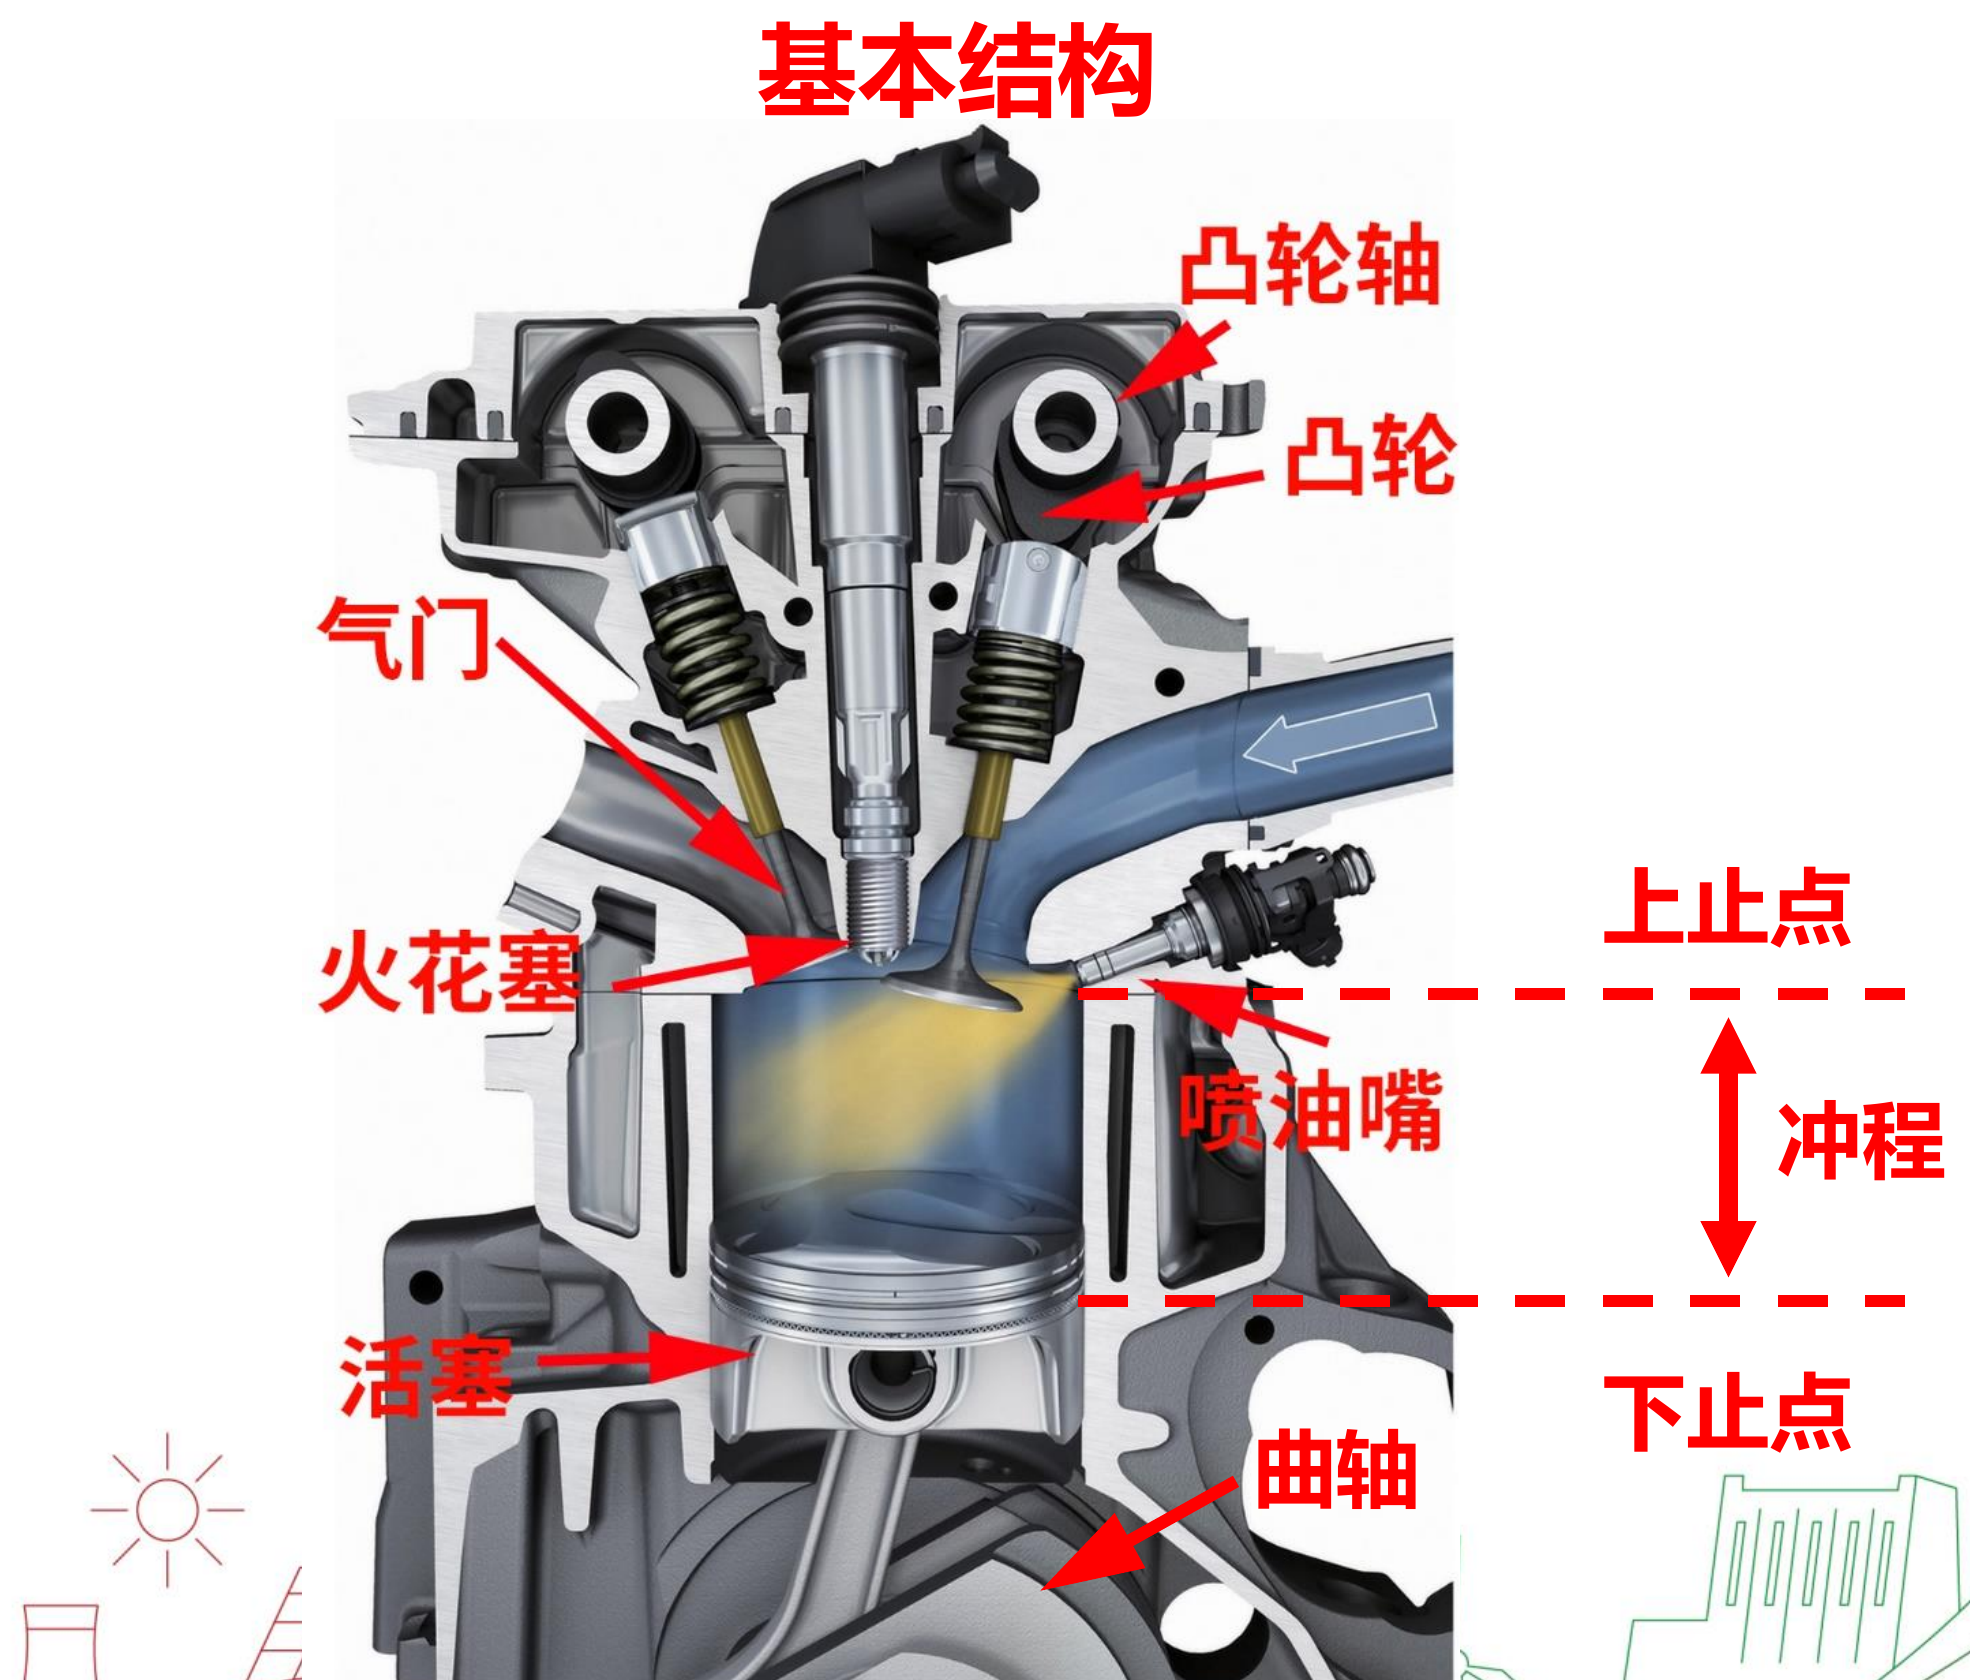
\includegraphics[height=46mm,keepaspectratio]{figures/course/engine_structure.png}
  \figcap{原课件第 62 页结构图局部；已保留主要标注。}
\end{column}
\begin{column}{0.59\textwidth}
  \begin{itemize}
    \item 活塞、连杆、曲轴：承受气体力，形成旋转输出。
    \item 凸轮轴、气门：控制换气时序。
    \item 火花塞 / 喷油器：对应点燃或压燃、缸外或缸内供油。
    \item 冷却、润滑：保障温度与摩擦状态。
  \end{itemize}
  \vspace{0.5mm}
  \begin{keybox}{读图顺序}
  \small 先找活塞—连杆—曲轴的运动链，再找凸轮—气门的换气链，最后看燃料与点火装置。
  \end{keybox}
\end{column}
\end{columns}
\end{frame}

%! src=63 kind=orig title=上、下止点与活塞行程
\begin{frame}[t,shrink]{\src{63}{上、下止点与活塞行程}}
\begin{columns}[T,onlytextwidth]
\begin{column}{0.50\textwidth}
  \begin{itemize}
    \item \textbf{上止点}：活塞顶离曲轴回转中心最远的位置。
    \item \textbf{下止点}：活塞顶离曲轴回转中心最近的位置。
    \item 在上、下止点处，活塞瞬时速度为零。
    \item 活塞行程 \(S\)：上、下止点之间的距离；曲柄半径为 \(R\)。
  \end{itemize}
  \vspace{0.5mm}
  \begin{keybox}{几何关系}
  \small 对于气缸中心线通过曲轴回转中心的机构：
  $$
  S=2R
  $$
  \end{keybox}
\end{column}
\begin{column}{0.47\textwidth}
\begin{center}
\begin{tikzpicture}[x=1mm,y=1mm,scale=0.9,transform shape]
  \draw[thick,black!55] (0,0) rectangle (20,38);
  \fill[black!25] (2,31) rectangle (18,34);
  \fill[black!10] (2,9) rectangle (18,12);
  \draw[<->,thin] (24,9) -- (24,34);
  \node[lab,anchor=west] at (24.5,21.5) {\(S\)};
  \draw[dashline] (18,34) -- (26,34);
  \draw[dashline] (18,9) -- (26,9);
  \node[lab,anchor=west] at (26,34) {上止点};
  \node[lab,anchor=west] at (26,9) {下止点};
  \draw[thick,black!55] (10,-4) circle (5);
  \draw[thick,black!55] (10,-4) -- (10,9);
  \draw[thick,cprimary] (10,-4) -- (15,-4);
  \node[lab,text=cprimary,anchor=south] at (13,-4) {\(R\)};
  \node[lab,anchor=north] at (10,-10) {曲柄半径 \(R\)};
\end{tikzpicture}
\end{center}
\figcap{活塞在上、下止点之间移动的距离为行程 \(S\)。}
\end{column}
\end{columns}
\end{frame}

%! src=63 kind=supp title=行程、转速与平均活塞速度
\begin{frame}[t,shrink]{\srcsupp{63}{行程、转速与平均活塞速度}}
曲轴每转一周，活塞累计移动距离为 \(2S\)，因此：
$$
\bar c_{\mathrm{p}}=\frac{2Sn}{60}
$$
\begin{columns}[T,onlytextwidth]
\begin{column}{0.51\textwidth}
  \begin{itemize}
    \item \(S\) 用 \(\mathrm{m}\)，\(n\) 用 \(\mathrm{r/min}\)，平均活塞速度为 \(\mathrm{m/s}\)。
    \item 平均速度概括运动强度；瞬时速度随曲轴转角变化。
    \item 止点处瞬时速度为零，不代表平均速度为零。
    \item 行程对应直线运动，转速对应曲轴转动，必须通过机构关系联系。
  \end{itemize}
\end{column}
\begin{column}{0.46\textwidth}
  \begin{keybox}{补充算例}
  \small 取 \(S=90\,\mathrm{mm}=0.09\,\mathrm{m}\)，\(n=3000\,\mathrm{r/min}\)：
  $$
  \bar c_{\mathrm{p}}=\frac{2\times0.09\times3000}{60}=9\,\mathrm{m/s}
  $$
  \end{keybox}
  \vspace{0.6mm}
  \begin{amberbox}{边界}
  \small 这里的平均速度是“累计路程/时间”，不是往复周期内平均速度矢量。
  \end{amberbox}
\end{column}
\end{columns}
\end{frame}

%! src=64 kind=orig title=工作容积、排量与燃烧室容积
\begin{frame}[t,shrink]{\src{64}{工作容积、排量与燃烧室容积}}
\begin{columns}[T,onlytextwidth]
\begin{column}{0.52\textwidth}
  \begin{smalltab}
  \begin{tabularx}{\linewidth}{@{}>{\bfseries}p{26mm}X@{}}
    \toprule
    名称 & 含义\\
    \midrule
    气缸工作容积 \(V_{\mathrm{s}}\) & 活塞从上止点移到下止点扫过的容积\\
    内燃机排量 \(V_{\mathrm{disp}}\) & 所有气缸工作容积之和\\
    燃烧室容积 \(V_{\mathrm{c}}\) & 活塞在上止点时，活塞顶以上的剩余容积\\
    \bottomrule
  \end{tabularx}
  \end{smalltab}
  \vspace{0.6mm}
  $$
  V_{\mathrm{s}}=\frac{\pi D^2}{4}S,
  \qquad
  V_{\mathrm{disp}}=zV_{\mathrm{s}}
  $$
  \begin{itemize}
    \item \(D\) 为缸径，\(z\) 为气缸数。
    \item 排量不包含燃烧室容积。
  \end{itemize}
\end{column}
\begin{column}{0.45\textwidth}
\begin{center}
\begin{tikzpicture}[x=1mm,y=1mm,scale=0.9,transform shape]
  \draw[thick,black!55] (0,0) rectangle (28,50);
  \fill[cblue!28] (0,45) rectangle (28,50);
  \fill[cprimary!18] (0,20) rectangle (28,45);
  \fill[black!30] (1,20) rectangle (27,24);
  \draw[dashline] (0,45) -- (28,45);
  \node[lab,anchor=west] at (29,47.5) {\(V_{\mathrm{c}}\)};
  \node[lab,anchor=west] at (29,32) {\(V_{\mathrm{s}}\)};
  \node[lab,anchor=west] at (29,21) {活塞};
  \node[lab,anchor=north] at (14,-2) {下止点位置};
\end{tikzpicture}
\end{center}
\figcap{气缸工作容积是活塞扫过的圆柱体积；燃烧室容积在活塞上止点以上。}
\end{column}
\end{columns}
\end{frame}

%! src=64 kind=supp title=用几何关系检查排量与单位
\begin{frame}[t,shrink]{\srcsupp{64}{用几何关系检查排量与单位}}
$$
V_{\mathrm{s}}=\frac{\pi D^2S}{4},
\qquad
V_{\mathrm{disp}}=z\frac{\pi D^2S}{4}
$$
\begin{columns}[T,onlytextwidth]
\begin{column}{0.51\textwidth}
  \begin{itemize}
    \item 缸径平方乘行程，因此同时放大缸径和行程，会显著改变排量。
    \item 缸径、行程必须先统一长度单位，再计算容积。
    \item \(1\,\mathrm{L}=10^{-3}\,\mathrm{m^3}=10^3\,\mathrm{cm^3}\)。
    \item 排量是几何参数，功率还取决于转速、充气与每循环输出功。
  \end{itemize}
\end{column}
\begin{column}{0.46\textwidth}
  \begin{keybox}{检查顺序}
  \small 先统一单位 $\rightarrow$ 算单缸 \(V_{\mathrm{s}}\) $\rightarrow$ 乘缸数得排量 $\rightarrow$ 再与压缩比所需的 \(V_{\mathrm{c}}\) 区分。
  \end{keybox}
  \vspace{0.6mm}
  \begin{amberbox}{符号}
  \small 这里的 \(D\) 是缸径；锅炉章节的 \(D\) 是蒸发量。跨章节阅读时要重新确认符号。
  \end{amberbox}
\end{column}
\end{columns}
\end{frame}

%! src=65 kind=orig title=气缸总容积与压缩比
\begin{frame}[t,shrink]{\src{65}{气缸总容积与压缩比}}
以 \(V_{\mathrm{c}}\) 表示燃烧室容积，\(V_{\mathrm{a}}\) 表示下止点时的总容积：
$$
V_{\mathrm{a}}=V_{\mathrm{s}}+V_{\mathrm{c}}
$$
$$
\varepsilon=\frac{V_{\mathrm{a}}}{V_{\mathrm{c}}}
=1+\frac{V_{\mathrm{s}}}{V_{\mathrm{c}}}
$$
\begin{columns}[T,onlytextwidth]
\begin{column}{0.47\textwidth}
  \begin{itemize}
    \item 压缩比 \(\varepsilon\) 是无量纲几何参数。
    \item 其他条件相同时，压缩比增大意味着压缩终了压力、温度更高。
    \item \textbf{压缩比是容积比}，不能直接当作压缩前后压力之比。
  \end{itemize}
\end{column}
\begin{column}{0.50\textwidth}
  \begin{keybox}{理想等熵关系}
  \small 若把缸内气体视为定比热理想气体，并近似为等熵压缩：
  $$
  \frac{T_2}{T_1}=\varepsilon^{\kappa-1},
  \qquad
  \frac{p_2}{p_1}=\varepsilon^{\kappa}
  $$
  这只是补充的理想模型，实际还受换热、泄漏和充气影响。
  \end{keybox}
\end{column}
\end{columns}
\end{frame}

%! src=66 kind=orig title=喷油与点火时序
\begin{frame}[t,shrink]{\src{66}{喷油与点火时序}}
\begin{center}
\begin{tikzpicture}[x=0.16mm,y=1mm,xshift=18mm]
  \fill[cblue!7] (0,2) rectangle (180,20);
  \fill[cprimary!7] (180,2) rectangle (360,20);
  \fill[camber!10] (360,2) rectangle (540,20);
  \fill[black!5] (540,2) rectangle (720,20);
  \foreach \y in {14,9,4}{\fill[white] (0,\y-1.2) rectangle (720,\y+1.2);}
  \foreach \y/\n in {14/气道喷射,9/缸内直喷,4/柴油机}{
    \node[lab,anchor=east] at (-2,\y) {\n};
  }
  \draw[thin,black!40] (0,2)--(720,2);
  \foreach \x in {180,360,540}{\draw[dashline] (\x,2)--(\x,20);}
  \node[lab,anchor=south] at (90,20) {进气};
  \node[lab,anchor=south] at (270,20) {压缩};
  \node[lab,anchor=south] at (450,20) {做功};
  \node[lab,anchor=south] at (630,20) {排气};
  % PFI
  \draw[cblue,thick] (30,12) -- (30,16);
  \draw[cprimary,thick] (350,12) -- (350,16);
  % GDI
  \draw[cblue,thick] (320,7) -- (320,11);
  \draw[cprimary,thick] (350,7) -- (350,11);
  % Diesel
  \draw[camber,thick] (340,2) -- (340,6);
  \foreach \x/\t in {0/0,180/180,360/360,540/540,720/720}{
    \draw[thin] (\x,2)--(\x,1);
    \node[lab,anchor=north] at (\x,1) {\t};
  }
  \node[lab,anchor=north] at (360,-5) {曲轴转角 / \((^\circ)\)};
\end{tikzpicture}
\end{center}
\begin{columns}[T,onlytextwidth]
\begin{column}{0.55\textwidth}
  \begin{itemize}
    \item 气道喷射汽油机：燃油在气道形成混合气，进气过程带入气缸，压缩末期火花点火。
    \item 缸内直喷汽油机：燃油直接喷入气缸，图示在压缩阶段，仍需火花点火。
    \item 柴油机：先压缩空气，压缩末期喷油，依靠高温空气压燃（不设火花塞）。
  \end{itemize}
\end{column}
\begin{column}{0.42\textwidth}
  \begin{keybox}{图例}
  \small \textcolor{cblue}{\rule{2mm}{1.6pt}} 喷油；\quad
  \textcolor{cprimary}{\rule{2mm}{1.6pt}} 火花点火；\quad
  \textcolor{camber}{\rule{2mm}{1.6pt}} 柴油喷油。
  \par\vspace{1mm}
  实际时刻随转速、负荷和排放策略变化，图中位置只是示意。
  \end{keybox}
\end{column}
\end{columns}
\end{frame}

%! src=67 kind=orig title=四冲程工作循环
\begin{frame}[t,shrink]{\src{67}{四冲程工作循环}}
\begin{columns}[T,onlytextwidth]
\begin{column}{0.60\textwidth}
  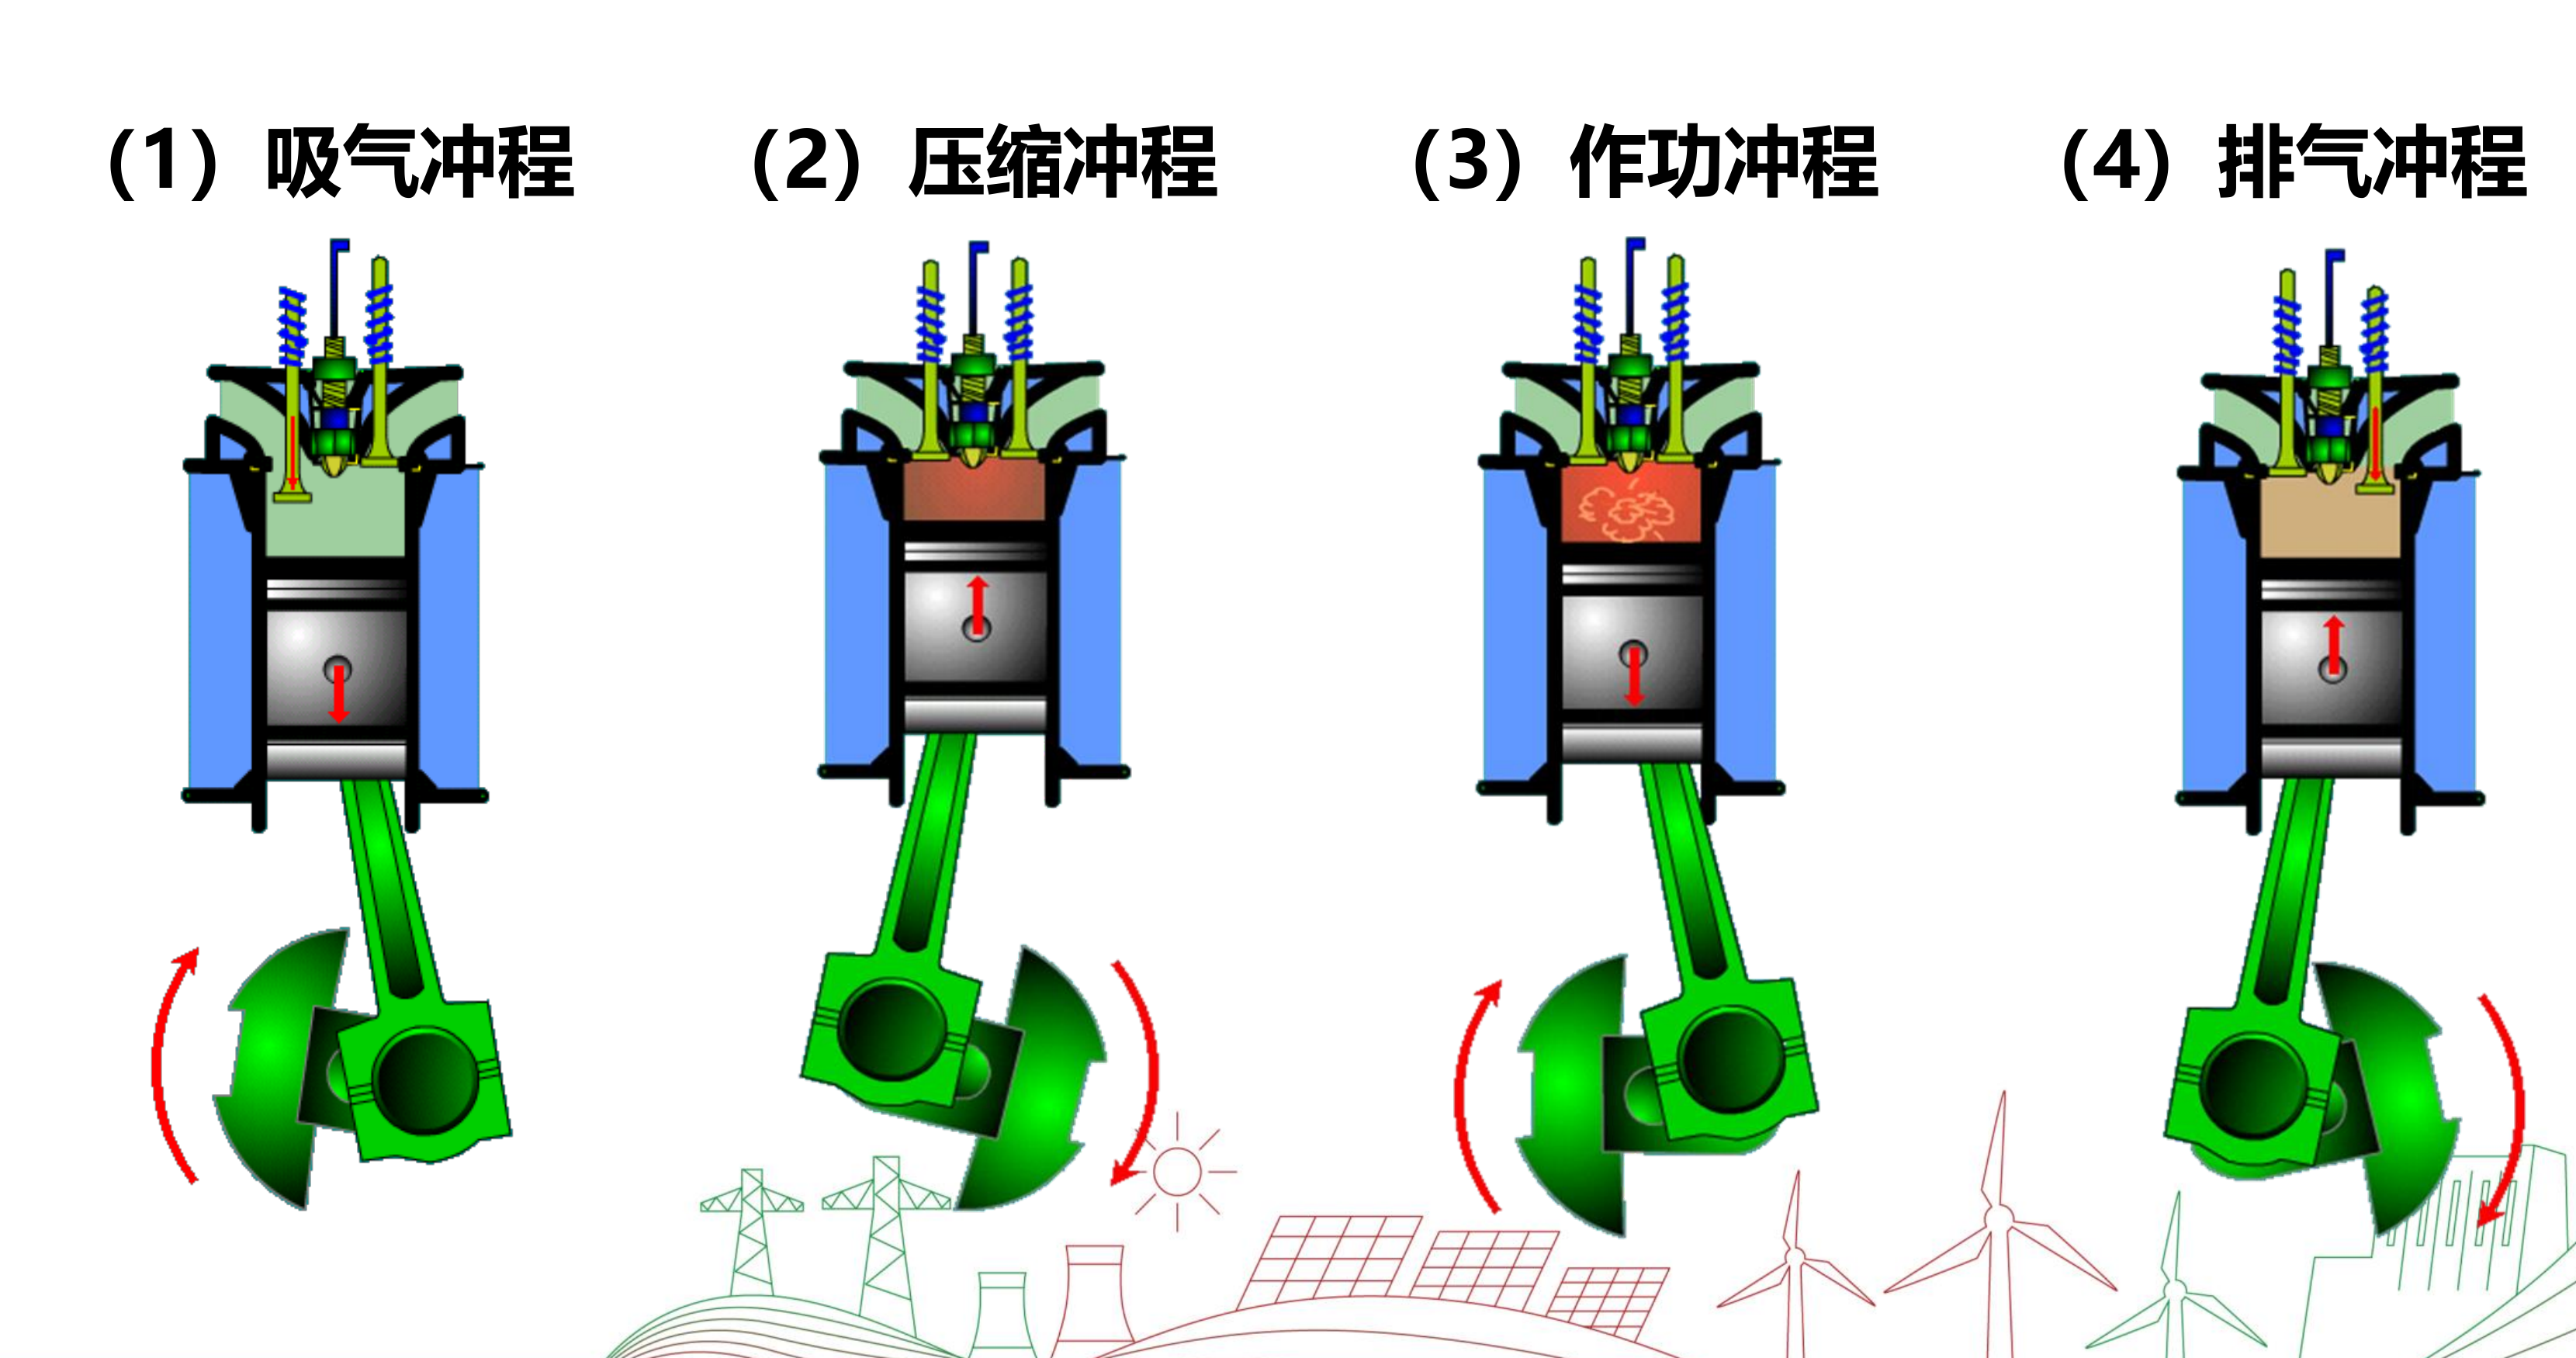
\includegraphics[width=\linewidth]{figures/course/four_stroke.png}
  \figcap{原课件第 67 页四冲程示意图；已保留四个冲程标题。}
\end{column}
\begin{column}{0.37\textwidth}
  \begin{smalltab}
  \begin{tabularx}{\linewidth}{@{}>{\bfseries}p{11mm}X@{}}
    \toprule
    冲程 & 主要过程\\
    \midrule
    进气 & 进气门开，吸入新鲜充量\\
    压缩 & 气门关，压缩气体\\
    做功 & 燃烧膨胀，推动活塞\\
    排气 & 排气门开，排出废气\\
    \bottomrule
  \end{tabularx}
  \end{smalltab}
  \begin{itemize}
    \item 一个循环曲轴转两周，即 \(720^\circ\)。
    \item 每缸每循环做功一次。
  \end{itemize}
\end{column}
\end{columns}
\end{frame}

%! src=67 kind=supp title=四冲程的做功频率
\begin{frame}[t,shrink]{\srcsupp{67}{四冲程的做功频率}}
每缸每两转完成一个工作循环。转速为 \(n\,\mathrm{r/min}\) 时：
$$
f_{\mathrm{cycle}}=\frac{n}{120}\,\mathrm{s^{-1}}
$$
若每缸每循环有效功为 \(W_{\mathrm{e,cyc}}\)，缸数为 \(z\)：
$$
P_{\mathrm{e}}=zW_{\mathrm{e,cyc}}\frac{n}{120}
$$
\begin{columns}[T,onlytextwidth]
\begin{column}{0.50\textwidth}
  \begin{itemize}
    \item \(W_{\mathrm{e,cyc}}\) 用 \(\mathrm{J}\)，所得 \(P_{\mathrm{e}}\) 为 \(\mathrm{W}\)。
    \item 四冲程每缸每两转做功一次；二冲程每转一次。
    \item 做功频率加倍不意味着同尺寸、同转速下功率必然严格加倍。
  \end{itemize}
\end{column}
\begin{column}{0.47\textwidth}
  \begin{keybox}{曲轴转角}
  \small 四冲程：进气 \(0\sim180^\circ\)，压缩 \(180\sim360^\circ\)，做功 \(360\sim540^\circ\)，排气 \(540\sim720^\circ\)（理想化划分）。
  \end{keybox}
\end{column}
\end{columns}
\end{frame}

%! src=68 kind=orig title=二冲程工作循环
\begin{frame}[t,shrink]{\src{68}{二冲程工作循环}}
\begin{columns}[T,onlytextwidth]
\begin{column}{0.60\textwidth}
  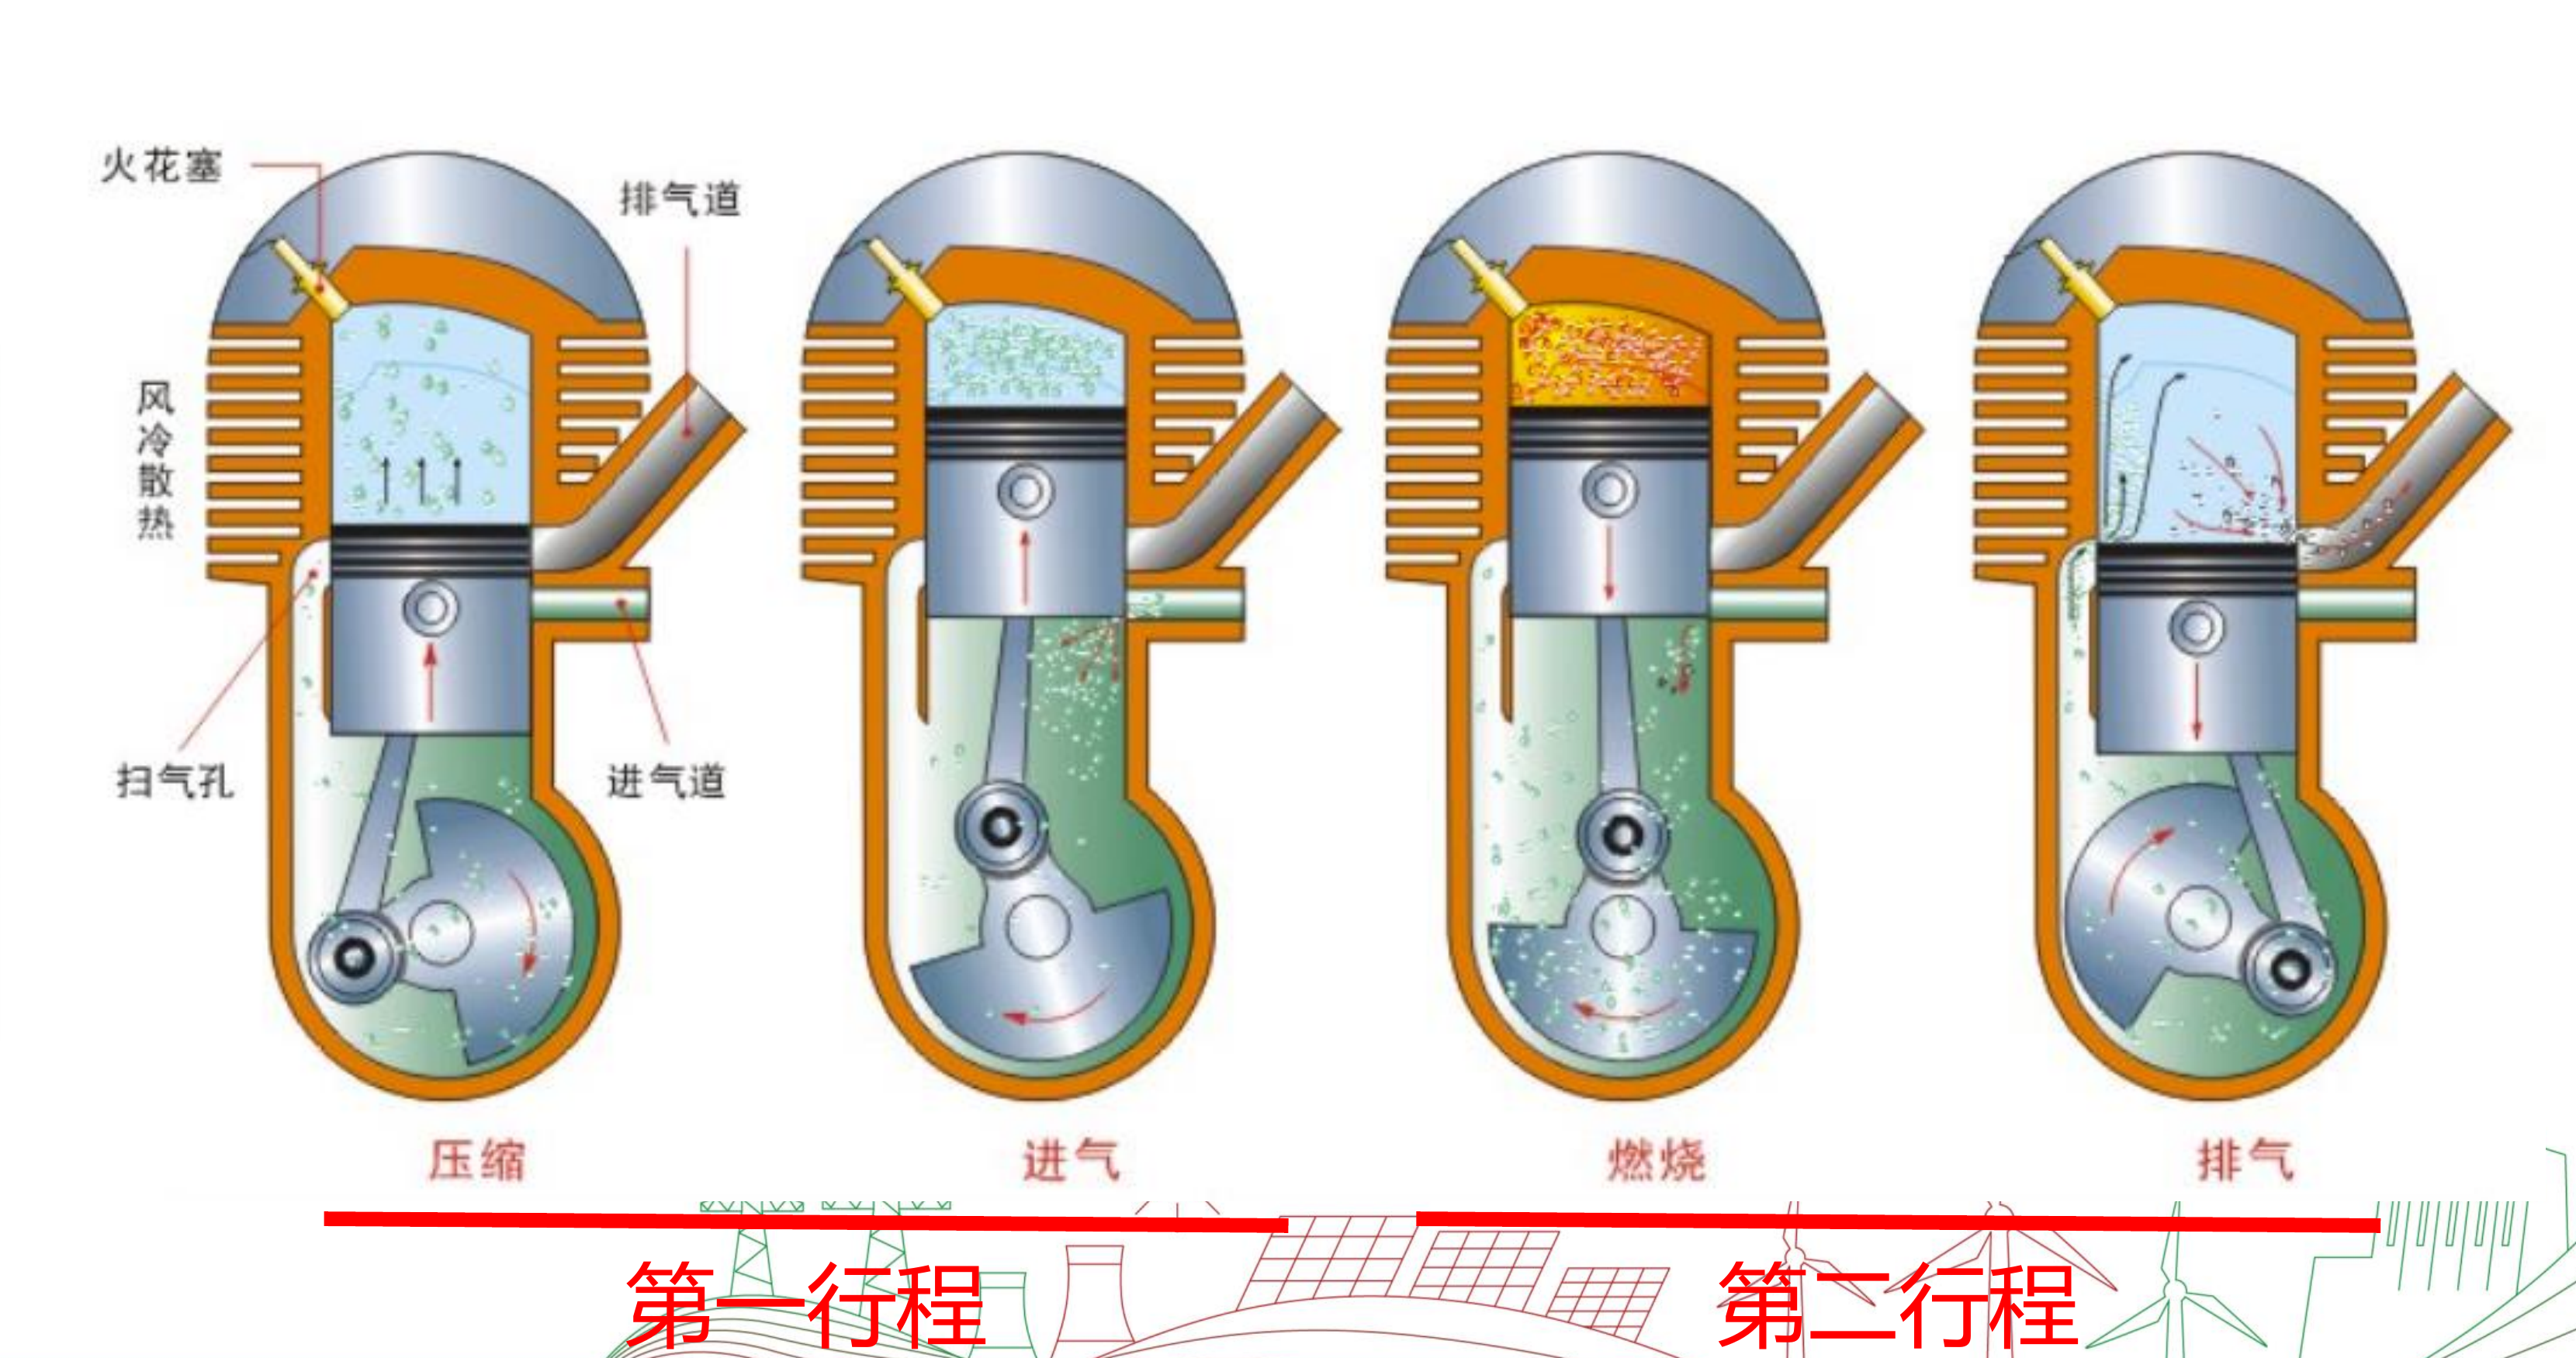
\includegraphics[width=\linewidth]{figures/course/two_stroke.png}
  \figcap{原课件第 68 页二冲程示意图；进排气口与扫气孔同时可见。}
\end{column}
\begin{column}{0.37\textwidth}
  \begin{itemize}
    \item 第一行程，活塞上行：缸内混合气压缩，曲轴箱吸入新鲜混合气。
    \item 上止点附近点火燃烧，进入第二行程。
    \item 第二行程，活塞下行：燃气膨胀做功，曲轴箱内充量受压。
    \item 下止点附近排气口、扫气口相继开启，进行排气与扫气。
    \item 一个循环曲轴转一周，即 \(360^\circ\)。
  \end{itemize}
\end{column}
\end{columns}
\end{frame}

%! src=68 kind=supp title=二冲程的扫气与循环重叠
\begin{frame}[t,shrink]{\srcsupp{68}{二冲程的扫气与循环重叠}}
\begin{itemize}
  \item 上行：缸内压缩，同时曲轴箱吸入新鲜充量；下行：膨胀做功，同时为后续扫气准备充量。
  \item 下止点附近：排气与扫气在相近时段发生；每缸每转一个循环，频率为 \(n/60\)。
  \item 二冲程的换气与其他过程重叠；图示结构不能概括所有二冲程发动机（如直流扫气、回流扫气等）。
\end{itemize}
\begin{center}
\begin{tikzpicture}[x=0.32mm,y=1.4mm]
  \fill[cprimary!15] (0,0.5) rectangle (160,4.5);
  \fill[camber!18] (160,0.5) rectangle (220,4.5);
  \fill[cblue!12] (220,0.5) rectangle (360,4.5);
  \draw[thin] (0,0.5) rectangle (360,4.5);
  \node[lab] at (80,6.1) {膨胀};
  \node[lab] at (190,6.1) {排气 / 扫气重叠};
  \node[lab] at (290,6.1) {压缩};
  \draw[thin] (160,0.5)--(160,7);
  \draw[thin] (220,0.5)--(220,7);
  \draw[axis] (0,0) -- (370,0);
  \foreach \x/\t in {0/0,180/180,360/360}{\draw[thin] (\x,0)--(\x,-1);\node[lab,anchor=north] at (\x,-1) {\t};}
  \node[lab,anchor=north] at (180,-6) {曲轴转角 / \((^\circ)\)};
\end{tikzpicture}
\end{center}
\figcap{补充时序示意：换气与膨胀/压缩存在重叠，不对应具体发动机配气时刻。}
\end{frame}

%! src=69 kind=orig title=汽油机与柴油机比较
\begin{frame}[t,shrink]{\src{69}{汽油机与柴油机比较}}
本页比较对象是典型\textbf{四冲程}汽油机与柴油机。
\begin{smalltab}
\begin{tabularx}{\linewidth}{@{}>{\bfseries}p{30mm}XX@{}}
  \toprule
  项目 & 汽油机 & 柴油机\\
  \midrule
  典型关键部件 & 火花塞 & 喷油器\\
  进气内容 & 传统气道供油时为混合气 & 主要为空气\\
  点火方式 & 点燃式 & 压燃式\\
  课件压缩比示例 & \(8\sim11\) & \(13\sim18\)\\
  每缸工作循环 & 四冲程、两周、做功一次 & 四冲程、两周、做功一次\\
  \bottomrule
\end{tabularx}
\end{smalltab}
\begin{columns}[T,onlytextwidth]
\begin{column}{0.53\textwidth}
  \begin{itemize}
    \item 缸内直喷汽油机的进气应结合第 66 页理解，不能套用“都吸入混合气”。
    \item 课件将优点简写为汽油机轻便、柴油机便宜且功率大；这些比较依具体机型而变。
  \end{itemize}
\end{column}
\begin{column}{0.44\textwidth}
  \begin{amberbox}{压缩比不是唯一判据}
  \small 压缩比、燃料性质、喷射方式和排放控制共同决定机型差异，不能只看一个数字。
  \end{amberbox}
\end{column}
\end{columns}
\end{frame}

%! src=70 kind=orig title=有效转矩与有效功率
\begin{frame}[t,shrink]{\src{70}{有效转矩与有效功率}}
\begin{columns}[T,onlytextwidth]
\begin{column}{0.51\textwidth}
  \begin{itemize}
    \item \textbf{有效转矩} \(T_{\mathrm{e}}\)：克服摩擦、附件驱动等损失后，曲轴输出的净转矩，单位 \(\mathrm{N\cdot m}\)。
    \item \textbf{有效功率} \(P_{\mathrm{e}}\)：曲轴或飞轮对外输出的净功率，单位 \(\mathrm{kW}\)。
    \item 功率等于转矩乘角速度，测得转矩和转速后即可计算。
  \end{itemize}
\end{column}
\begin{column}{0.46\textwidth}
  \begin{keybox}{基本关系}
  \small
  $$
  P_{\mathrm{e}}=T_{\mathrm{e}}\omega,
  \qquad
  \omega=\frac{2\pi n}{60}
  $$
  常用单位：
  $$
  \frac{P_{\mathrm{e}}}{\mathrm{kW}}
  \approx\frac{1}{9550}
  \left(\frac{T_{\mathrm{e}}}{\mathrm{N\cdot m}}\right)
  \left(\frac{n}{\mathrm{r/min}}\right)
  $$
  \end{keybox}
\end{column}
\end{columns}
\vspace{0.5mm}
\begin{amberbox}{区分“指示”和“有效”}
\small 指示功率是缸内气体对活塞做功的功率；有效功率是扣除机械损失后从曲轴输出的功率。
\end{amberbox}
\end{frame}

%! src=70 kind=supp title=9550 系数从哪里来
\begin{frame}[t,shrink]{\srcsupp{70}{9550 系数从哪里来}}
当 \(n\) 用 \(\mathrm{r/min}\)，\(T_{\mathrm{e}}\) 用 \(\mathrm{N\cdot m}\) 时：
$$
P_{\mathrm{e}}\,[\mathrm{W}]
=T_{\mathrm{e}}\frac{2\pi n}{60}
$$
$$
P_{\mathrm{e}}\,[\mathrm{kW}]
=\frac{T_{\mathrm{e}}n}{60\times1000/(2\pi)}
\approx\frac{T_{\mathrm{e}}n}{9550}
$$
\begin{columns}[T,onlytextwidth]
\begin{column}{0.50\textwidth}
  \begin{itemize}
    \item \(60\) 把每分钟换为每秒；\(1000\) 把瓦换为千瓦。
    \item \(60\times1000/(2\pi)=9549.3\ldots\)，工程上取 9550。
    \item 转矩大不一定功率大，还要看转速。
  \end{itemize}
\end{column}
\begin{column}{0.47\textwidth}
  \begin{amberbox}{单位陷阱}
  \small 使用角速度 \(\omega\) 时，直接用 \(P=T\omega\)，不要再除以 9550；9550 只适用于 \(\mathrm{N\cdot m}\)、\(\mathrm{r/min}\)、\(\mathrm{kW}\) 这组单位。
  \end{amberbox}
\end{column}
\end{columns}
\end{frame}

%! src=71 kind=orig title=热效率与有效燃油消耗率
\begin{frame}[t,shrink]{\src{71}{热效率与有效燃油消耗率}}
$$
\eta_{\mathrm{t}}=\frac{P_{\mathrm{i}}}{\dot m_{\mathrm{f}}H_{\mathrm{u}}},
\qquad
\eta_{\mathrm{e}}=\frac{P_{\mathrm{e}}}{\dot m_{\mathrm{f}}H_{\mathrm{u}}}
$$
\begin{columns}[T,onlytextwidth]
\begin{column}{0.50\textwidth}
  \begin{itemize}
    \item 课件用 \(\eta_{\mathrm{t}}\) 表示\textbf{指示热效率}：燃料热量转为缸内指示功的比例。
    \item 有效热效率：转为曲轴有效功的比例，计入机械损失后更低。
    \item \(\dot m_{\mathrm{f}}\)：燃油质量流量；\(H_{\mathrm{u}}\)：低位发热量。
  \end{itemize}
\end{column}
\begin{column}{0.47\textwidth}
  \begin{keybox}{有效燃油消耗率}
  \small
  $$
  \frac{g_{\mathrm{e}}}{\mathrm{g/(kW\cdot h)}}
  =3.6\times10^6
  \frac{\dot m_{\mathrm{f}}/\mathrm{(kg/s)}}{P_{\mathrm{e}}/\mathrm{kW}}
  $$
  \end{keybox}
\end{column}
\end{columns}
\vspace{0.5mm}
\begin{amberbox}{符号提醒}
\small 原课件用 \(\eta_{\mathrm{t}}\) 指“指示热效率”，下标容易与温度 \(t\) 混淆；本整理在补充中改用 \(\eta_{\mathrm{i}}\) 表示同一含义。
\end{amberbox}
\end{frame}

%! src=71 kind=supp title=指示效率、有效效率与油耗率
\begin{frame}[t,shrink]{\srcsupp{71}{指示效率、有效效率与油耗率的关系}}
定义机械效率 \(\eta_{\mathrm{m}}=P_{\mathrm{e}}/P_{\mathrm{i}}\)，有：
$$
\eta_{\mathrm{e}}=\eta_{\mathrm{i}}\eta_{\mathrm{m}},
\qquad
\frac{g_{\mathrm{e}}}{\mathrm{g/(kW\cdot h)}}
=\frac{3.6\times10^6}
{\eta_{\mathrm{e}}\left(H_{\mathrm{u}}/\mathrm{(kJ/kg)}\right)}
$$
\begin{columns}[T,onlytextwidth]
\begin{column}{0.50\textwidth}
  \begin{itemize}
    \item 第一式区分缸内指示功与曲轴有效功，是定义的直接结果。
    \item 第二式在油耗用 \(\mathrm{g/(kW\cdot h)}\)、低位热值用 \(\mathrm{kJ/kg}\) 时成立。
    \item 同一种燃料下，油耗率降低对应有效热效率提高。
    \item 比较不同燃料时应先考虑低位热值，不能只比较质量油耗率。
  \end{itemize}
\end{column}
\begin{column}{0.46\textwidth}
  \begin{keybox}{量纲检查}
  \small \(g_{\mathrm{e}}H_{\mathrm{u}}\) 的单位为 \(\mathrm{g\cdot kJ/(kW\cdot h)}\)；换算后与 \(3.6\times10^6\) 的系数对应。
  \end{keybox}
\end{column}
\end{columns}
\end{frame}

%! src=72 kind=orig title=结束页与复习自检
\begin{frame}[t,shrink]{\src{72}{结束页与复习自检}}
原页为“谢谢”，没有新增知识点。用以下问题串联全篇：
\begin{columns}[T,onlytextwidth]
\begin{column}{0.55\textwidth}
  \begin{enumerate}
    \item 画出蒸汽电厂的能量转换链、风烟流程和汽水流程。
    \item 区分锅炉三种流动方式，列出六项热平衡输出。
    \item 解释速度三角形、反动度、级损失与相对内效率。
    \item 说明凝汽器维持真空的作用，以及经济真空的权衡。
    \item 写出布雷顿循环四过程，说明增压比与温比的不同影响。
    \item 区分行程、排量、压缩比，并用转矩、转速计算功率。
  \end{enumerate}
\end{column}
\begin{column}{0.41\textwidth}
  \begin{keybox}{复习重点}
  \small 先说明系统边界与假设，再使用公式和经验数据。
  \end{keybox}
  \vspace{4mm}
  \begin{center}
  {\Huge\bfseries\textcolor{cprimary}{谢谢}}
  \end{center}
\end{column}
\end{columns}
\end{frame}

\input{sections/06_close.tex}

\end{document}
